\chapter{Theory of Sets}

\section{COLLECTIVIZING RELATIONS}

\subsection{THE THEORY OF SETS}

The theory of sets is a theory which contains the relational signs \(=,\) \(\in\) and the substantific sign \(\supset\) (all these signs being of weight 2); in addition to the schemes S1 to S7 given in Chapter I, it contains the scheme S8, which will be introduced in no. 6, and the explicit axioms A1 (no. 3.) A2 (no. 5), A3 ( \(\S\) 2, no. 1), A4 ( \(\S\) 5, no. 1), and A5 (Chapter III, \(\S\) 6, no. 1), These explicit axioms contain no letters; in other words, the theory of sets is a theory without constants.

Since the theory of sets is an equalitarian theory, the results of Chapter I are applicable.

From now on, unless the contrary is expressly stated, we shall always argue in a theory which is stronger (Chapter I, §2, no. 4) than the theory of sets; if the theory is not mentioned, it is to be assumed that the theory of sets is implied. It will be evident in many cases that this hypothesis is superfluous, and the reader should have no difficulty in determining in what theory weaker than the theory of sets the results stated are valid.

If T and U are terms, the assembly \(\in TU\) is a relation (called the relation of membership) which in practice we write in one of the following ways: \(\widetilde{T} \in U\) , \((\widetilde{T}) \in (U)\) , ``T belongs to U'', ``T is an element of U''. The relation ``not \((\widetilde{T} \in U)\) '' is written \(T \notin U\) .

From a ``naive'' point of view, many mathematical entities can be considered as collections or ``sets'' of objects. We do not seek to formalize this notion, and in the formalistic interpretation of what follows, the word ``set'' is to be considered as strictly synonymous with ``term''. In particular, phrases such as ``let X be a set'' are, in principle, quite superfluous, since every letter is a term. Such phrases are introduced only to assist the intuitive interpretation of the text.

\subsection{INCLUSION}

DEFINITION 1. The relation denoted by \((\forall z)((z \in x) \Longrightarrow (z \in y))\) , in which only the letters \(x\) and \(y\) appear, is written in one of the following ways: \(x \subset y\) , \(y \supset x\) , `` \(x\) is contained in \(y\) '', `` \(y\) contains \(x\) '', `` \(x\) is a subset of \(y\) ''. The relation ``not \((x \subset y)\) '' is written \(x \not\subset y\) or \(y \not\supset x\) .

In accordance with the conventions mentioned in Chapter I, §1, no. 1, this definition entails the following metamathematical convention. Let T and U be assemblies; if we substitute T for x and U for y in the assembly \(x \subset y\) , we obtain an assembly which is denoted by \(T \subset U\) ; if we denote by x, y letters which are distinct from x, y and distinct from each other, and which appear neither in T nor in U, the assembly \(T \subset U\) is then identical with \((T|x)(U|y)(x|x)(y|y)(x \subset y,)\) and hence by CS8, CS9 (Chapter I, §4, no. 1), and CS5 (Chapter I, §1, no. 2) with \((\forall z)((z \in T) \Longrightarrow (z \in U))\) , provided that z is a letter which appears neither in T nor in U.

From now on, whenever we state a mathematical definition, we shall not mention the metamathematical convention which it entails.

CS12. Let \(\pmb{T},\pmb{U},\pmb{V}\) be assemblies and let \(\pmb{x}\) be a letter. Then the assembly \((\pmb{V}|\pmb{x})(\pmb{T}\subset \pmb{U})\) is identical with \((\pmb{V}|\pmb{x})\pmb{T}\subset (\pmb{V}|\pmb{x})\pmb{U}\) .

This follows immediately from CS9 (Chapter I, § 4, no. 1) and CS5 (Chapter I, § 1, no. 2).

CF13. If \(\pmb{T}\) and \(\pmb{U}\) are terms, \(\pmb{T} \subset \pmb{U}\) is a relation.

This follows immediately from CF8 (Chapter I, §1, no. 4).

¶ Every relation of the form \(T \subset U\) (where T and U are terms) is called an inclusion relation.

From now on we shall no longer write down explicitly the criteria of substitution and the formative criteria which should follow the definitions. It should be noted, however, that these criteria will often be used implicitly in proofs.

To prove the relation \(x \subset y\) in a theory \(\mathfrak{G}\) , it is enough, by C27 (Chapter I, §4, no. 1), to prove that \(z \in y\) in the theory obtained by adjoining \(z \in x\) to the axioms of \(\mathfrak{G}\) , where \(z\) is a letter distinct from \(x, y\) and the constants of the theory. In practice we say ``let \(z\) be an element of \(x\) '', and we attempt to prove \(z \in y\) .

PROPOSITION 1. \(x \subset x\) .

Obvious.

PROPOSITION 2. \((x\subset y\) and \(y\subset z)\Longrightarrow (x\subset z).\)

Adjoin the hypotheses \(x \subset y, y \subset z\) , and \(u \in x\) . Then the relations

\[
(u \in x) \Longrightarrow (u \in y), \quad (u \in y) \Longrightarrow (u \in z),
\]

are true, and therefore the relation \(u \in z\) is true.

\subsection{THE AXIOM OF EXTENT}

The axiom of extent is the following axiom :

A1.

\[
(\forall x) (\forall y) ((x \subset y \text {   and   } y \subset x) \Longrightarrow (x = y)).
\]

Intuitively, this axiom expresses the fact that two sets which have the same elements are equal.

To prove that x = y it is therefore enough to prove \(z \in y\) in the theory obtained by adjoining the hypothesis \(z \in x\) , and \(z \in x\) in the theory obtained by adjoining the hypothesis \(z \in y\) , where z is a letter distinct from x, y, and the constants.

C48. Let R be a relation, x a letter, and y a letter distinct from x which does not appear in R. Then the relation \((\forall x)((x \in y) \Longleftrightarrow R)\) is single-valued in y.

Let \(\pmb{z}\) be a letter distinct from \(\pmb{x}\) which does not appear in \(\pmb{R}\) . Adjoin the hypotheses

\[
(\forall x) ((x \in y) \Longleftrightarrow R), (\forall x) ((x \in z) \Longleftrightarrow R).
\]

Then we have successively the theorems

\[
\begin{array}{c} (\forall x) (((x \in y) \Longleftrightarrow R) \quad \text { and } \quad ((x \in z) \Longleftrightarrow R)), \\ (\forall x) ((x \in y) \Longleftrightarrow (x \in z)), \\ y \subset z, \qquad z \subset y. \end{array}
\]

By A1 we have then y = z. This proves C48.

\subsection{COLLECTIVIZING RELATIONS}

Let R be a relation and let x be a letter. If y and \(y'\) denote letters distinct from x which do not appear in R, then the relations

\[
(\exists y) (\forall x) ((x \in y) \leftrightarrow R), (\exists y ^ {\prime}) (\forall x) ((x \in y ^ {\prime}) \leftrightarrow R)
\]

are identical by CS8 (Chapter I, §4, no. 1). The relation thus defined (which does not contain x) is denoted by Coll \(_{x}\) R.

If \(\operatorname{Coll}_{\mathbf{x}} R\) is a theorem in a theory \(\mathcal{G}\) , \(R\) is said to be collectivizing in \(\mathbf{x}\) in \(\mathcal{G}\) . When this is so, we may introduce an auxiliary constant \(\mathbf{a}\) , distinct from \(\mathbf{x}\) and the constants of \(\mathcal{G}\) , and which does not appear in \(\mathbf{R}\) , with the introductory axiom \((\forall \mathbf{x}) ((\mathbf{x} \in \mathbf{a}) \Longleftrightarrow \mathbf{R})\) , or equivalently (if \(\mathbf{x}\) is not a constant of \(\mathcal{G}\) ) \((\mathbf{x} \in \mathbf{a}) \Longleftrightarrow \mathbf{R}\) .

Intuitively, to say that R is collecting in x is to say that there exists a set a such that the objects x which possess the property R are precisely the elements of a.

\minorheading{Examples}

\begin{enumerate}
\def\labelenumi{(\arabic{enumi})}
\item
  The relation \(x \in y\) is clearly collectivizing in \(x\) .
\item
  The relation \(x \notin x\) is not collectivizing in \(x\) ; in other words, (not \(\operatorname{Coll}_x(x \notin x)\) ) is a theorem. Let us argue by contradiction and suppose that \(x \notin x\) is collectivizing. Let \(a\) be an auxiliary constant, distinct from \(x\) and the constants of the theory, with the introductory axiom
\end{enumerate}

\[
(\forall x) ((x \notin x) \iff (x \in a)).
\]

Then the relation

\[
(a \notin a) \iff (a \in a)
\]

is true by C30 (Chapter I, §4, no. 3). The method of disjunction of cases (Chapter I, §3, no. 3) shows first that the relation \(\pmb{a} \notin \pmb{a}\) is true, and then that the relation \(\pmb{a} \in \pmb{a}\) is true, which is absurd.

C49. Let R be a relation and x a letter. If R is collectivizing in x, the relation \((\forall x)((x \in y) \Longleftrightarrow R)\) , where y is a letter distinct from x which does not appear in R, is functional in y.

This follows immediately from C48.

Very often in what follows we shall have at our disposal a theorem of the form \(Coll_{x}R\) . To represent the term

\[
\tau_ {y} (\forall x) ((x \in y) \iff R),
\]

which does not depend on the choice of the letter y (distinct from x and not appearing in R), we shall introduce a functional symbol \(\mathcal{E}\mathbf{x}(\mathbf{R})\) ; the corresponding term does not contain X. This term is denoted by ``the set of all x such that R''. By definition (Chapter I, §4, no. 1) the relation

\[
(\forall x) ((x \in \mathcal {E} x (R)) \iff R)
\]

is identical with \(Coll_{x}R\) ; consequently the relation R is equivalent to

\[
\boldsymbol {x} \in \mathcal {E} _ {\boldsymbol {x}} (\boldsymbol {R}).
\]

C50. Let R, S be two relations and let x be a letter. If R and S are collectivizing in x, the relation \((\forall x)(R \Longrightarrow S)\) is equivalent to

\[
\mathcal {E} _ {\boldsymbol {x}} (\boldsymbol {R}) \subset \mathcal {E} _ {\boldsymbol {x}} (\boldsymbol {S}),
\]

and the relation \((\forall x)(R \Longleftrightarrow S)\) is equivalent to \(\mathcal{E}_{x}(R) = \mathcal{E}_{x}(S)\) .

This follows immediately from the preceding remark and from Definition 1 and axiom A1.

\subsection{THE AXIOM OF THE SET OF TWO ELEMENTS}

\[
(\forall x) (\forall y) \operatorname{Coll} _ {z} (z = x \text {   or   } z = y).
\]

This axiom says that if \(x\) and \(y\) are objects, then there is a set whose only elements are \(x\) and \(y\) .

DEFINITION 2. The set \(\mathfrak{E}_z\) ( \(z = x\) or \(z = y\) ), whose only elements are \(x\) and \(y\) , is denoted by \(\{x, y\}\) .

The relation \(z \in \{x, y\}\) is therefore equivalent to `` \(z = x\) or \(z = y\) ''; it follows from C50 that \(\{y, x\} = \{x, y\}\) .

Let \(R\{z\}\) be a relation and let \(x, y\) be letters distinct from \(z\) . From the criteria C32, C33 (Chapter I, §4, no. 3), and C43 (Chapter I, §5, no. 1) it follows easily that the relation \((\exists z)((z \in \{x, y\})\) and \(R\{z\})\) is equivalent to `` \(R\{x\}\) or \(R\{y\}\) ''; consequently the relation \((\forall z)((z \in \{x, y\}) \Longrightarrow R\{z\})\) is equivalent to `` \(R\{x\}\) and \(R\{y\}\) ''.

The set \(\{x, x\}\) , which is denoted simply by \(\{x\}\) , is called the set whose only element is x; the relation \(z \in \{x\}\) is equivalent to z = x, and the relation \(x \in X\) is equivalent to \(\{x\} \subset X\) .

\subsection{THE SCHEME OF SELECTION AND UNION}

The scheme of selection and union is the following :

S8. Let R be a relation, let x and y be distinct letters, and let X and Y be letters distinct from x and y which do not appear in R. Then the relation

\[
(1) \quad (\forall y) (\exists X) (\forall x) (R \Longrightarrow (x \in X)) \Longrightarrow (\forall Y) \operatorname{Coll} _ {X} ((\exists y) ((y \in Y) \text {   and   } R))
\]

is an axiom.

Let us first show that this rule is indeed a scheme. Let \(S\) denote the relation (1), and let us substitute a term \(T\) for a letter \(z\) in \(S\) ; by CS8 (Chapter I, §4, no. 1) we may suppose that \(x, y, X, Y\) are distinct from \(z\) and do not appear in \(T\) . Then \((T|z)S\) is identical with

\[
(\forall y) (\exists X) (\forall x) (R ^ {\prime} \Longrightarrow (x \in X)) \Longrightarrow (\forall Y) \operatorname{Coll} _ {X} ((\exists y) ((y \in Y) \text {   and   } R ^ {\prime})),
\]

where \(R'\) is \((T|z)R\) .

Intuitively, the relation \((\forall y)(\exists X)(\forall x)(R \Rightarrow (x \in X))\) means that for every object \(y\) there exists a set \(X\) (which may depend on \(y\) ) such that the objects \(x\) which are in the relation \(R\) with the given object \(y\) are elements of \(X\) (but not necessarily the whole of \(X\) ). The scheme of selection and union asserts that if this is the case and if \(Y\) is any set, then there exists a set whose elements are precisely the objects \(x\) which are in the relation \(R\) with at least one object \(y\) of the set \(Y\) .

C51. Let P be a relation, let A be a set, and let x be a letter which does not appear in A. Then the relation ``P and \(x \in A\) '' is collectivizing in x.

Let R denote the relation ``P and x = y'', where y is a letter distinct from x which appears neither in P nor in A. The relation

\[
(\forall x) (R \Longrightarrow (x \in \{y \}))
\]

is true by C27 (Chapter I, §4, no. 1). Let \(X\) be a letter distinct from \(x\) and \(y\) which does not appear in \(P\) . The preceding relation is identical with \((\{y\}|X)((\forall x)(R \Longrightarrow (x \in X)))\) (because \(x\) is distinct from \(y\) ), and therefore the relation \((\forall y)(\exists X)(\forall x)(R \Longrightarrow (x \in X))\) is true by virtue of S5 and C27 (Chapter I, §4, nos. 1 and 2). It follows from S8 and C30 (Chapter I, §4, no. 3) that the relation

\[
(A | Y) \operatorname{Coll} x (\exists y) (y \in Y \text {   and   } R)
\]

(where Y is a letter which does not appear in R) is true, and this relation is identical with \(\operatorname{Coll}_{\mathbf{x}}(\exists\mathbf{y})(\mathbf{y}\in\mathbf{A}\) and R) (because neither x nor y appears in A). Finally, the relation `` \(y\in A\) and R'' is equivalent to ``x=y and \(x\in A\) and P'' by C43 (Chapter I, §5, no. 1); since x appears neither in P nor in A, the relation

\[
(\exists y) (x = y \text {   and   } x \in A \text {   and   } P)
\]

is equivalent to ``((∃y)(x=y)) and x∈A and P'' by C33 (Chapter I, §4, no. 3) and therefore to ``P and x∈A'' because (∃y)(x=y) is true.

The set \(\mathcal{E}_{\pmb{x}}(\pmb{P}\) and \(\pmb{x} \in \pmb{A})\) is called the set of all \(\pmb{x} \in \pmb{A}\) such that \(\pmb{P}\) (* thus we may speak of the set of all real numbers such that \(\pmb{P}_{*}\) ).

C52. Let R be a relation, A a set, and x a letter which does not appear in A. If the relation \(R \Longrightarrow (x \in A)\) is a theorem, then R is collectivizing in x.

For R is then equivalent to ``R and \(x \in A\) ''.

Remark. Let R be a relation which is collectivizing in x, and let S be a relation such that \((\forall x)(S \Longrightarrow R)\) is a theorem. Then S is collectivizing in x; for R is equivalent to \(x \in \mathcal{E}_{x}(R)\) , so that

\[
S \Longrightarrow (x \in \mathcal {E} _ {x} (R))
\]

is a theorem, and the assertion follows from C52. Notice also that in this case we have \(\mathcal{E}_{\pmb{X}}(\pmb{S}) \subset \mathcal{E}_{\pmb{X}}(\pmb{R})\) by C50.

C53. Let T be a term, A a set, x and y distinct letters. Suppose that x does not appear in A and that y does not appear in A nor in T. Then the relation \((\exists x)(y = T \text{ and } x \in A)\) is collectivizing in y.

Let R be the relation y = T. The relation \((\forall y)(R \Longrightarrow (y \in \{T\}))\) is true, hence so is \((\forall x)(\exists X)(\forall y)(R \Longrightarrow (y \in X))\) , where X is a letter, distinct from y, which does not appear in R. By virtue of S8, the relation \((\exists x)(x \in A \text{ and } R)\) is collectivizing in y, and C53 is proved.

The relation \((\exists x)(y = T\) and \(x \in A)\) is often read as follows: ``y can be put in the form \(T\) for some \(x\) belonging to \(A\)''. The set

\[
\mathcal {E} _ {\boldsymbol {y}} ((\exists \boldsymbol {x}) (\boldsymbol {y} = \boldsymbol {T} \text {   and   } \boldsymbol {x} \in A))
\]

is generally called the set of objects of the form T for \(x \in A\) . The assembly so denoted contains neither x nor y, and does not depend on the choice of the letter y satisfying the conditions of C53.

\subsection{COMPLEMENT OF A SET. THE EMPTY SET}

The relation \((x \notin A \text{ and } x \in X)\) is collectivizing in x by C51.

DEFINITION 3. Let A be a subset of a set X. The set of elements of X which do not belong to A, that is to say the set \(\mathfrak{E}\mathbf{x}\) ( \(x \notin \mathrm{A}\) and \(x \in \mathrm{X}\) ), is called the complement of A in X, and is denoted by \(\complement_{\mathbf{X}}\mathrm{A}\) or \(\mathrm{X} - \mathrm{A}\) (or by \(\complement\mathrm{A}\) if there is no risk of confusion).

Let A be a subset of a set X; the relations `` \(x \in X\) and \(x \notin A\) '' and \(x \in \complement_{X} A\) are then equivalent. Consequently the relation `` \(x \in X\) and \(x \notin \complement_{X} A\) '' is equivalent to `` \(x \in X\) and ( \(x \notin X\) or \(x \in A\) )'', hence to \(x \in A\) . In other words, \(A = \complement_{\mathbf{X}}(\complement_{\mathbf{X}} A)\) is a true relation. Similarly, one shows that if \(B\) is a subset of \(X\) , the relations \(A \subset B\) and \(\complement_{\mathbf{X}} B \subset \complement_{\mathbf{X}} A\) are equivalent.

THEOREM 1. The relation \((\forall x)(x \notin X)\) is functional in \(X\) .

For the relation \((\forall x)(x \notin X)\) implies \((\forall Y)(X \subset Y)\) ; by virtue of the axiom of extent, the relation \((\forall x)(x \notin X)\) is therefore single-valued in \(X\) . On the other hand, the relation \((\forall x)(x \notin C_{Y}Y)\) is true, which proves that \((\exists X)(\forall x)(x \notin X)\) is true.

The term \(\tau_x((\forall x)(x \notin X))\) corresponding to this functional relation is represented by the functional symbol \(\phi\) , and is called the empty set (*); the relation \((\forall x)(x \notin X)\) , which is equivalent to \(X = \phi\) , is read as follows: ``the set \(X\) is empty''. We have the theorems \(x \notin \phi\) , \(\phi \subset X\) , \(\complement_X X = \phi\) , \(\complement_X \phi = X\) . The relation \(X \subset \phi\) is equivalent to \(X = \phi\) . If \(R \{x\}\) is a relation, the relation \((\forall x)((x \in \phi) \Longrightarrow R \{x\})\) is true.

Remark. There exists no set of which every object is an element; in other words, ``not \((\exists X)(\forall x)(x \in X)\) '' is a theorem. For if there were such a set, then by C52 every relation would be collectivizing. But we have seen (no. 4) that the relation \(x \notin x\) is not collectivizing.

\section{ORDERED PAIRS}

\subsection{THE AXIOM OF THE ORDERED PAIR}

As we have said in §1, no. 1, the sign \(\supset\) is a substantific sign of weight 2 in the theory of sets. If T, U are terms, then \(\supset\) TU is a term, which in practice is denoted by (T, U). In this notation, the axiom of the ordered pair is the following :

\[
(\forall x) (\forall x ^ {\prime}) (\forall y) (\forall y ^ {\prime}) (((x, y) = (x ^ {\prime}, y ^ {\prime})) \Longrightarrow (x = x ^ {\prime} \quad \text { and } \quad y = y ^ {\prime})). \tag {A3.}
\]

Since the relation `` \(x = x'\) and \(y = y'\)'' implies \((x, y) = (x', y')\) by C44 (Chapter I, § 5, no. 2), the relation \((x, y) = (x', y')\) is equivalent to `` \(x = x'\) and \(y = y'\)''.

¶ The relation \((\exists x)(\exists y)(z=(x,y))\) is written ``z is an ordered pair''. If z is an ordered pair, the relations

\[
(\exists y) (z = (x, y)), \quad (\exists x) (z = (x, y))
\]

are functional with respect to \(x\) and \(y\) respectively; this is an immediate consequence of A3.

The terms

\[
\tau_ {x} ((\exists y) (z = (x, y))) \quad \text { and } \quad \tau_ {y} ((\exists x) (z = (x, y)))
\]

are denoted by \(\mathbf{pr}_1z\) and \(\mathbf{pr}_2z\) , respectively, and are called the first coordinate (or first projection) and the second coordinate (or second projection) of \(z\) . If \(z\) is an ordered pair, the relation \((\exists y)(z = (x, y))\) is equivalent to \(x = \mathbf{pr}_1z\) , and the relation \((\exists x)(z = (x, y))\) to \(y = \mathbf{pr}_2z\) (Chapter I, §5, no. 3).

The relation \(z = (x, y)\) is equivalent to `` \(z\) is an ordered pair, and \(x = \text{pr}_1z\) and \(y = \text{pr}_2z\) ''; for the latter relation is equivalent to

\[
(\exists x ^ {\prime}) (\exists y ^ {\prime}) (\exists x ^ {\prime \prime}) (\exists y ^ {\prime \prime}) (z = (x ^ {\prime}, y ^ {\prime}) \text {   and   } z = (x, y ^ {\prime \prime}) \text {   and   } z = (x ^ {\prime \prime}, y));
\]

by A3, `` \(z = (x', y')\) and \(z = (x, y'')\) and \(z = (x'', y)\)'' is equivalent to `` \(z = (x, y)\) and \(x = x'\) and \(x = x''\) and \(y = y'\) and \(y = y''\) ''; hence by C33 (Chapter I, §4, no. 3), `` \(z\) is an ordered pair, and \(x = \text{pr}_1 z\) and \(y = \text{pr}_2 z\) '' is equivalent to

\[
z = (x, y) \text { and } (\exists x ^ {\prime}) (\exists y ^ {\prime}) (\exists x ^ {\prime \prime}) (\exists y ^ {\prime \prime}) (x = x ^ {\prime} \text { and } x = x ^ {\prime \prime} \text { and } y = y ^ {\prime} \text { and } y = y ^ {\prime \prime}),
\]

which proves our assertion. Evidently we have

\[
\operatorname{pr} _ {1} (x, y) = x, \quad \operatorname{pr} _ {2} (x, y) = y,
\]

and the relation \(z = (\mathrm{pr}_1(z), \mathrm{pr}_2(z))\) is equivalent to `` \(z\) is an ordered pair''.

Let \(R\{x, y\}\) be a relation, where the letters x and y are distinct and appear in R. Let z be a letter, distinct from x and y, which does not appear in R. Let \(S\{z\}\) denote the relation

\[
(\exists x) (\exists y) (z = (x, y) \text {   and   } R \{x, y \});
\]

this is a relation which contains one letter fewer than R, and which is equivalent to ``z is an ordered pair and \(R\{pr_{1}z, pr_{2}z\}\) '', this follows from the fact that \(z = (x, y)\) is equivalent to ``z is an ordered pair and \(x = pr_{1}x\) and \(y = pr_{2}z\) '', and from criteria C33 (Chapter I, §4, no. 3)

and C47 (Chapter I, §5, no. 3). It follows immediately that \(R\{x, y\}\) is equivalent to \(S\{(x, y)\}\) , and also to

\[
(\exists z) (z = (x, y) \text {   and   } S \{z \})
\]

by C47.

This means that we may interpret a relation between the objects x and y as a property of the ordered pair formed by these objects.

\subsection{PRODUCT OF TWO SETS}

THEOREM 1. The relation

\[
(\forall \mathrm{X}) (\forall \mathrm{Y}) (\exists \mathrm{Z}) (\forall z) ((z \in \mathrm{Z}) \iff (\exists x) (\exists y) (z = (x, y) \text {   and   } x \in \mathrm{X} \text {   and   } y \in \mathrm{Y})
\]

is true. In other words, for all X and all Y the relation ``z is an ordered pair and \(pr_{1}z \in X\) and \(pr_{2}z \in Y\) '' is collectivizing in z.

Let \(A_y\) denote the set of all objects of the form \((x, y)\) for \(x \in X\) (cf.~§1, no. 6, criterion C53). Let \(R\) be the relation \(z \in A_y\) , which is equivalent to \((\exists x)(z = (x, y)\) and \(x \in X)\) . It is clear that the relation

\[
(\forall y) (\exists \mathrm{A}) (\forall z) (\mathrm{R} \Longrightarrow (z \in \mathrm{A}))
\]

is true, by virtue of S5 (Chapter I, §4, no. 2). It then follows from S8 that the relation \((\exists y)(y \in \mathbf{Y}\) and \(\mathbf{R})\) is collectivizing in \(z\) . But this relation is equivalent to \((\exists x)(\exists y)(y \in \mathbf{Y}\) and \(x \in \mathbf{X}\) and \(z = (x, y)\) ); hence the result.

DEFINITION 1. Given two sets X and Y, the set

\[
\mathcal {E} _ {z} ((\exists x) (\exists y) (z = (x, y) \text {   and   } x \in X \text {   and   } y \in Y))
\]

is called the product of X and Y and is denoted by \(X \times Y\) .

The relation \(z \in X \times Y\) is thus equivalent to `` \(z\) is an ordered pair and \(\text{pr}_1z \in X\) and \(\text{pr}_2z \in Y\) ''. The sets \(X\) and \(Y\) are called the first and second factors of \(X \times Y\) .

PROPOSITION 1. If A', B' are non-empty sets, the relation A' × B' ⊂ A × B is equivalent to ``A' ⊂ A and B' ⊂ B''.

In the first place, the relation \(z \in A' \times B'\) is equivalent to `` \(z\) is an ordered pair and \(\mathrm{pr}_1z \in A'\) and \(\mathrm{pr}_2z \in B'\)''; therefore, without any restriction on \(A'\) and \(B'\) , the relation `` \(A' \subset A\) and \(B' \subset B\)'' implies

\[
\mathbf {A} ^ {\prime} \times \mathbf {B} ^ {\prime} \subset \mathbf {A} \times \mathbf {B}.
\]

Conversely, let us first show that if \(B' \neq \emptyset\) (without restriction on \(A'\) ), the relation \(A' \times B' \subset A \times B\) implies \(A' \subset A\) . Let x be an element of \(A'\) ; since \(B' \neq \emptyset\) , there is an object y which is an element of \(B'\) ; we have \((x, y) \in A' \times B'\) , hence \((x, y) \in A \times B\) , and consequently \(x \in A\) ; thus \(A' \subset A\) . Similarly, if \(A' \neq \emptyset\) , the relation \(A' \times B' \subset A \times B\) implies \(B' \subset B\) . Hence the result.

PROPOSITION 2. Let A and B be two sets. The relation \(\mathbf{A} \times \mathbf{B} = \varnothing\) is equivalent to `` \(\mathbf{A} = \varnothing\) or \(\mathbf{B} = \varnothing\) ''.

For the relation \(z \in A \times B\) implies \(\mathsf{pr}_1z \in A\) and \(\mathsf{pr}_2z \in B\) ; hence \(A \neq \emptyset\) and \(B \neq \emptyset\) . Conversely, the relation `` \(x \in A\) and \(y \in B\) '' implies \((x, y) \in A \times B\) and hence \(A \times B \neq \emptyset\) . In other words, the relation \(A \times B \neq \emptyset\) is equivalent to `` \(A \neq \emptyset\) and \(B \neq \emptyset\) ''; hence the result.

If A, B, C are sets, we write

\[
(\mathbf {A} \times \mathbf {B}) \times \mathbf {C} = \mathbf {A} \times \mathbf {B} \times \mathbf {C};
\]

an element \(((x, y), z)\) of A × B × C is written \((x, y, z)\) and is called a triple. Again, if A, B, C, D are sets, we write

\[
(\mathbf {A} \times \mathbf {B} \times \mathbf {C}) \times \mathbf {D} = \mathbf {A} \times \mathbf {B} \times \mathbf {C} \times \mathbf {D};
\]

and so on.

\section{CORRESPONDENCES}

\subsection{GRAPHS AND CORRESPONDENCES}

DEFINITION 1. G is said to be a graph if every element of G is an ordered pair, i.e., if the relation

\[
(\forall z) (z \in G \Longrightarrow (z \text {   is   an   ordered   pair }))
\]

is true.

If G is a graph, the relation \((x, y) \in \mathbf{G}\) is expressed by saying that ``y corresponds to x under G''.

Let \(R \mid x, y \mid\) be a relation, where \(x\) and \(y\) are distinct letters. Let \(G\) be a letter, distinct from \(x\) and \(y\) , which does not appear in \(R\) . If the relation

\[
(\exists G) (G \text {   is   a   graph   and   } (\forall x) (\forall y) (R \Longleftrightarrow ((x, y) \in G)))
\]

is true, the relation R is said to have a graph (with respect to the letters x and y). The graph G is then unique by virtue of the axiom of extent, and is called the graph of R with respect to x and y.

Let \(\pmb{Z}\) be a letter, distinct from \(\pmb{x}\) and \(\pmb{y}\) , which does not appear in \(\pmb{R}\) . If the relation

\[
(\exists Z) (\forall x) (\forall y) (R \Longrightarrow ((x, y) \in Z))
\]

is true, then \(R\) has a graph; we may take this graph to be the set of ordered pairs \(z\) such that \(z \in Z\) and \(R \{ \text{pr}_1 z, \text{pr}_2 z \}\) ( \(z\) being a letter distinct from \(x, y, Z\) which does not appear in \(R\) ). This condition is satisfied if we know a term \(T\) , which does not contain either \(x\) or \(y\) , such that \(R \Longrightarrow ((x, y) \in T)\) is true.

PROPOSITION 1. Let G be a graph. There exists exactly one set A and exactly one set B with the following properties:

\begin{enumerate}
\def\labelenumi{(\arabic{enumi})}
\item
  the relation \((\exists y)((x, y) \in G)\) is equivalent to \(x \in A\) ;
\item
  the relation \((\exists x)((x, y) \in \mathbf{G})\) is equivalent to \(y \in \mathbf{B}\) .
\end{enumerate}

For it is sufficient to take A (resp. B) to be the set of all objects of the form \(pr_{1}z\) (resp. \(pr_{2}z\) ), where \(z \in G\) (§ 1, no. 6). Precisely,

\[
\mathrm{A} = \mathcal {E} _ {x} ((\exists y) ((x, y) \in \mathrm{G}))) \quad \text { and } \quad \mathrm{B} = \mathcal {E} _ {y} ((\exists x) ((x, y) \in \mathrm{G}));
\]

these sets are called respectively the first and second projections of the graph G, or the domain and range of G; they are denoted by \(pr_{1}\langle G\rangle\) and \(pr_{2}\langle G\rangle\) (or by \(pr_{1}G\) and \(pr_{2}G\) if there is no risk of confusion). It is immediately verified that \(G\subset(\mathrm{pr}_{1}\mathrm{G})\times(\mathrm{pr}_{2}\mathrm{G})\) ; every set of ordered pairs is therefore a subset of a product, and conversely. If one of the two sets \(pr_{1}G\) , \(pr_{2}G\) is empty, we have \(G=\varnothing\) (§2, Proposition 2).

Remark. The relation \(x = y\) has no graph, for the first projection of the graph, if it existed, would be the set of all objects (cf.~§1, no. 7, Remark).

\textbf{DEFINITION 2.} A correspondence between a set A and a set B is a triple

\[
\Gamma = (\mathrm{G}, \mathrm{A}, \mathrm{B}),
\]

where G is a graph such that \(pr_{1}G \subset A\) and \(pr_{2}G \subset B\) . G is said to be the graph of \(\Gamma\) , A is the source, and B the target of \(\Gamma\) .

If \((x, y) \in G\) , we say that ``y corresponds to x in the correspondence \(\Gamma\) ''. For each \(x \in pr_{1}G\) the correspondence \(\Gamma\) is said to be defined at x, and \(pr_{1}G\) is called the domain of \(\Gamma\) ; each \(y \in pr_{2}G\) is said to be a value taken by \(\Gamma\) , and \(pr_{2}G\) is called the range of \(\Gamma\) .

If \(R\{x, y\}\) is a relation which has a graph \(G\) (with respect to the letters \(x, y\) ), and if \(A, B\) are two sets such that \(\operatorname{pr}_1 G \subset A\) and \(\operatorname{pr}_2 G \subset B\) , we say that R is a relation between an element of A and an element of B (with respect to the letters x, y). The correspondence \(\Gamma = (G, A, B)\) is said to be the correspondence between A and B defined by the relation R (with respect to x and y).

Let \(\mathbf{G}\) be a graph and let \(\mathbf{X}\) be a set. The relation

\[
x \in \mathrm{X} \text {   and   } (x, y) \in \mathrm{G}
\]

implies \((x, y) \in G\) and therefore has a graph \(G'\) . The second projection of \(G'\) consists of all the objects which correspond under G to objects of X.

DEFINITION 3. Let G be a graph and X a set. The set of all objects which correspond under G to elements of X is called the image of X under G and is denoted by G⟨X⟩ or G(X).

Let \(\Gamma = (\mathbf{G},\mathbf{A},\mathbf{B})\) be a correspondence and let \(\mathbf{X}\) be a subset of \(\mathbf{A}\) . The set \(\mathbf{G}\langle \mathbf{X}\rangle\) is also denoted by \(\Gamma \langle \mathbf{X}\rangle\) or \(\Gamma (\mathbf{X})\) and is called the image of \(\mathbf{X}\) under \(\Gamma\) .

Remarks

\begin{enumerate}
\def\labelenumi{(\arabic{enumi})}
\item
  Precisely, \(\mathbf{G}\langle \mathbf{X}\rangle\) denotes the set \(\mathcal{E}_{\gamma}((\exists x)(x\in \mathbf{X}\) and \((x,y)\in \mathbf{G}))\) . From now on we shall not usually translate our definitions into formal language.
\item
  The notations G(X) and \(\Gamma(X)\) can occasionally lead to confusion with the notation introduced later (cf.~no. 4, Remark following Definition 9).
\end{enumerate}

Let G be a graph. Since the relation \((x, y) \in G\) implies \(y \in pr_{2}G\) , we have \(G\langle X \rangle \subset pr_{2}G\) for every set X. Since \((x, y) \in G\) implies \(x \in pr_{1}G\) , we have \(G\langle pr_{1}G \rangle = pr_{2}G\) . We have \(G\langle \phi \rangle = \phi\) , since \(x \notin \phi\) is a theorem. If \(X \subset pr_{1}G\) and \(X \neq \phi\) , we have \(G\langle X \rangle \neq \phi\) .

PROPOSITION 2. Let G be a graph and let X, Y be two sets; then the relation \(X \subset Y\) implies \(G\langle X\rangle \subset G\langle Y\rangle\) .

This is an immediate consequence of the definitions and of C50 (§ 1, no. 4).

COROLLARY. If \(\mathbf{A} \supset \mathrm{pr}_1\mathbf{G}\) , we have \(\mathbf{G}\langle \mathbf{A} \rangle = \mathrm{pr}_2\mathbf{G}\) .

DEFINITION 4. Let G be a graph and x an object. The set G\textless\{x\}\textgreater(which is sometimes denoted by G(x), by abuse of language) is called the section of G at x.

It follows immediately from C43 (Chapter I, § 5, no. 1) that the relation \(y \in G \langle \{x\} \rangle\) is equivalent to \((x, y) \in G\) . If \(G\) and \(G'\) are two graphs, the relation \(G \subset G'\) is thus equivalent to

\[
(\forall x) (\mathrm{G} \langle \{x \} \rangle \subset \mathrm{G} ^ {\prime} \langle \{x \} \rangle).
\]

If \(\Gamma = (G, A, B)\) is a correspondence between \(A\) and \(B\) , then for every \(x \in A\) the section of \(G\) at \(x\) is also called the section of \(\Gamma\) at \(x\) and is denoted by \(\Gamma \langle \{x\} \rangle\) (or \(\Gamma(x)\) ).

\subsection{INVERSE OF A CORRESPONDENCE}

Let \(G\) be a graph and \(A = \operatorname{pr}_1 G\) , \(B = \operatorname{pr}_2 G\) its projections. The relation \((y, x) \in G\) implies \((x, y) \in B \times A\) ; this relation therefore has a graph which consists of all ordered pairs \((x, y)\) such that \((y, x) \in G\) .

DEFINITION 5. Let G be a graph. The graph whose elements are the ordered pairs \((x, y)\) such that \((y, x) \in G\) is called the inverse of G and is denoted by \(\overline{G}\) .

For every set X, \(\overline{G}\langle X\rangle\) is called the inverse image of X under G.

It is clear that the inverse of \(\overline{G}\) is \(G\) , and that

\[
\mathrm{pr} _ {1} ^ {- 1} \mathrm{G} = \mathrm{pr} _ {2} \mathrm{G}, \quad \mathrm{pr} _ {2} ^ {- 1} \mathrm{G} = \mathrm{pr} _ {1} \mathrm{G}.
\]

In particular, if X, Y are two sets, we have

\[
\widehat {\mathbf {X} \times \mathbf {Y}} = \mathbf {Y} \times \mathbf {X}.
\]

A graph G is said to be symmetric if \(\overline{G}^{-1}=G\) .

Let \(\Gamma = (G, A, B)\) be a correspondence between \(A\) and \(B\) . Since \(\operatorname{pr}_1^{\overline{-1}} G \subset B\) and \(\operatorname{pr}_2^{\overline{-1}} G \subset A\) , the triple \((G, B, A)\) is a correspondence between \(B\) and \(A\) , called the inverse of the correspondence \(\Gamma\) , and denoted by \(\overline{\Gamma}\) . For every subset \(Y\) of \(B\) , the image \(\overline{\Gamma} \langle Y \rangle\) of \(Y\) under \(\overline{\Gamma}\) is also called the inverse image of \(Y\) under \(\Gamma\) . Clearly the inverse of \(\overline{\Gamma}\) is \(\Gamma\) .

\subsection{COMPOSITION OF TWO CORRESPONDENCES}

Let \(G, G'\) be two graphs. Let A denote the set \(pr_1G\) and let C denote the set \(pr_2G'\) . The relation \((\exists y)((x, y) \in G\) and \((y, z) \in G')\) implies that \((x, z) \in A \times C\) , and therefore has a graph with respect to x and z.

DEFINITION 6. Let G, G' be two graphs. The graph (with respect to x and z) of the relation \((\exists y)((x, y) \in G \text{ and } (y, z) \in G')\) is called the composition of G' and G, and is denoted by G' o G (or sometimes by G'G).

PROPOSITION 3. Let G, G' be two graphs. The inverse of G' o G is then \(\overline{G} \circ \overline{G'}\) .

For the relation `` \((x, y) \in G\) and \((y, z) \in G'\) '' is equivalent to

\[
(z, y) \in \overline {{\mathbf {G} ^ {\prime}}} \text {   and   } (y, x) \in \overline {{\mathbf {G}}}
\]

PROPOSITION 4. Let \(G_{1}\) , \(G_{2}\) , \(G_{3}\) be graphs. Then

\[
\left(\mathrm{G} _ {3} \circ \mathrm{G} _ {2}\right) \circ \mathrm{G} _ {1} = \mathrm{G} _ {3} \circ \left(\mathrm{G} _ {2} \circ \mathrm{G} _ {1}\right).
\]

The relation \((x, t) \in (\mathbf{G}_3 \circ \mathbf{G}_2) \circ \mathbf{G}_1\) is equivalent to the relation

\[
(\exists y) ((x, y) \in \mathrm{G} _ {1} \text {   and   } \exists z ((y, z) \in \mathrm{G} _ {2} \text {   and   } (z, t) \in \mathrm{G} _ {3}))
\]

and therefore (by C33 (Chapter I, §4, no. 3)) to the relation

\[
(\exists y) (\exists z) ((x, y) \in \mathrm{G} _ {1} \text {   and   } (y, z) \in \mathrm{G} _ {2} \text {   and   } (z, t) \in \mathrm{G} _ {3}).\tag{1}
\]

Similarly, the relation \((x, t) \in \mathbf{G}_3 \circ (\mathbf{G}_2 \circ \mathbf{G}_1)\) is equivalent to

\[
(\exists z) (\exists y) ((x, y) \in \mathrm{G} _ {1} \text {   and   } (y, z) \in \mathrm{G} _ {2} \text {   and   } (z, t) \in \mathrm{G} _ {3}).\tag{2}
\]

But the relations (1) and (2) are equivalent; hence the result.

¶ The graph \(G_{3} \circ (G_{2} \circ G_{1})\) is denoted by \(G_{3} \circ G_{2} \circ G_{1}\) . Similarly, if \(G_{1}, G_{2}, G_{3}, G_{4}\) are graphs, we put

\[
\mathrm{G} _ {4} \circ (\mathrm{G} _ {3} \circ \mathrm{G} _ {2} \circ \mathrm{G} _ {1}) = \mathrm{G} _ {4} \circ \mathrm{G} _ {3} \circ \mathrm{G} _ {2} \circ \mathrm{G} _ {1};
\]

and so on.

PROPOSITION 5. Let G, G' be graphs and let A be a set. Then

\[
(\mathbf {G} ^ {\prime} \circ \mathbf {G}) \langle \mathbf {A} \rangle = \mathbf {G} ^ {\prime} \langle \mathbf {G} \langle \mathbf {A} \rangle \rangle .
\]

For by virtue of C33 (Chapter I, § 4, no. 3) the relation \(z \in (\mathbf{G}' \circ \mathbf{G})\langle \mathbf{A} \rangle\) is equivalent to

\[
(\exists y) ((\exists x) (x \in A \text {   and   } (x, y) \in G) \text {   and   } (y, z) \in G ^ {\prime})
\]

and is therefore equivalent to \((\exists y)(y \in G \langle A \rangle\) and \((y, z) \in G')\) ; hence the result.

If G and \(G'\) are two graphs, we have \(\mathrm{pr}_{1}(\mathrm{G}' \circ \mathrm{G}) = \mathrm{G}\langle\mathrm{pr}_{1}\mathrm{G}'\rangle\) , and \(\mathrm{pr}_{2}(\mathrm{G}' \circ \mathrm{G}) = \mathrm{G}'\langle\mathrm{pr}_{2}\mathrm{G}\rangle\) . For example, to prove the second of these relations it is enough to note that the relation \(z \in \mathrm{pr}_2(G' \circ G)\) is equivalent to \((\exists x)((x, z) \in G' \circ G)\) and therefore to

\[
(\exists y) ((\exists x) ((x, y) \in G) \quad \text { and } \quad (y, z) \in G ^ {\prime});
\]

but this is equivalent to \(z \in G' \langle pr_{2}G \rangle\) .

If G is a graph and X a set such that \(X \subset pr_{1}G\) , we have

\[
\mathbf {X} \subset \overline {{\mathbf {G}}} \langle \mathbf {G} \langle \mathbf {X} \rangle \rangle .
\]

For the relation \(x \in \mathbf{X}\) implies by hypothesis that \((\exists y)((x, y) \in \mathbf{G})\) ; but \((x, y) \in \mathbf{G}\) is equivalent to \((y, x) \in \overline{\mathbf{G}}\) , and on the other hand \((x, y) \in \mathbf{G}\) implies \((\exists z)(z \in \mathbf{X} \text{ and } (z, y) \in \mathbf{G})\) ; hence \(x \in \mathbf{X}\) implies

\[
(\exists y) ((\exists z) (z \in X \text { and } (z, y) \in G) \text { and } (y, x) \in \overline {{G}} ^ {- 1}),
\]

that is to say, \(x \in \overline{\mathbf{G}}\langle \mathbf{G}\langle \mathbf{X}\rangle\rangle\) .

It is clear that if \(G_{1}\) , \(G_{2}\) , \(G_{1}^{\prime}\) , \(G_{2}^{\prime}\) are graphs, the relations \(G_{1} \subset G_{2}\) and \(G_{1}^{\prime} \subset G_{2}^{\prime}\) imply \(G_{1}^{\prime} \circ G_{1} \subset G_{2}^{\prime} \circ G_{2}\) .

Let \(\Gamma = (G, A, B)\) and \(\Gamma' = (G', B, C)\) be two correspondences such that the target of \(\Gamma\) is the same as the source of \(\Gamma'\) . From the above discussion we have \(\mathrm{pr}_1(G' \circ G) \subset \mathrm{pr}_1G \subset A\) and \(\mathrm{pr}_2(G' \circ G) \subset \mathrm{pr}_2G' \subset C\) ; hence we may state the following definition:

DEFINITION 7. Let \(\Gamma = (G, A, B)\) and \(\Gamma' = (G', B, C)\) be two correspondences such that the target of \(\Gamma\) is the source of \(\Gamma'\) . Then the correspondence \((G' \circ G, A, C)\) is called the composition of \(\Gamma'\) and \(\Gamma\) , and is denoted by \(\Gamma' \circ \Gamma\) (or sometimes \(\Gamma' \Gamma\) ).

It follows immediately from Proposition 5 that if X is a subset of A we have \((\Gamma'\circ\Gamma)\langle X\rangle=\Gamma'\langle\Gamma\langle X\rangle\rangle\) . Furthermore, since the target of \(\overline{\Gamma}^{1}\) is the same as the source of \(\overline{\Gamma}\) , the inverse of \(\Gamma'\circ\Gamma\) is \(\overline{\Gamma}\circ\overline{\Gamma}'\) , by Proposition 3.

DEFINITION 8. If A is a set, the set \(\Delta_{\mathbf{A}}\) of all objects of the form \((x, x)\) , where \(x \in \mathbf{A}\) , is called the diagonal of \(\mathbf{A} \times \mathbf{A}\) .

Clearly we have \(\mathrm{pr}_1\Delta_{\mathbf{A}} = \mathrm{pr}_2\Delta_{\mathbf{A}} = \mathbf{A}\) . The correspondence

\[
\mathbf {I} _ {\mathbf {A}} = (\Delta_ {\mathbf {A}}, \mathbf {A}, \mathbf {A})
\]

is called the identity correspondence on A; it is its own inverse.

If \(\Gamma\) is a correspondence between A and B and if \(I_{A}, I_{B}\) are the identity correspondences on A, B, respectively, then \(\Gamma \circ I_{A} = I_{B} \circ \Gamma = \Gamma\) .

\subsection{FUNCTIONS}

DEFINITION 9. A graph F is said to be a functional graph if for each x there is at most one object which corresponds to x under F (Chapter I, §5, no. 3). A correspondence \(f = (\mathbf{F}, \mathbf{A}, \mathbf{B})\) is said to be a function if its graph F is a functional graph and if its source A is equal to its domain \(\mathbf{pr}_1\mathbf{F}\) . In other words, a correspondence \(f = (\mathbf{F}, \mathbf{A}, \mathbf{B})\) is a function if for every x belonging to the source A of f the relation \((x, y) \in \mathbf{F}\) is functional in y (Chapter I, §5, no. 3); the unique object which corresponds to x under f is called the value of f at the element x of A, and is denoted by \(f(x)\) (or \(f_x\) , or \(\mathbf{F}(x)\) , or \(\mathbf{F}_x\) ).

If \(f\) is a function, \(F\) its graph, and \(x\) an element of the domain of \(f\) , the relation \(y = f(x)\) is then equivalent to \((x, y) \in F\) (Chapter I, §5, no. 3, criterion C46).

Remark. The reader should beware of the confusion which may arise from the simultaneous use of the notations \(f(x)\) and \(f(X)\) (synonymous with \(f\langle X\rangle\) ) introduced in Definition 3 (cf.~Exercise 11).

Let A and B be two sets; a mapping of A into B is a function f whose source (which is equal to its domain) is equal to A and whose target is equal to B; such a function is also said to be defined on A and to take its values in B.

Instead of the phrase ``let f be a mapping of A into B'', the following phrases are often used: ``let \(f: A \rightarrow B\) be a mapping'' or even ``let \(f: A \rightarrow B\) ''. To simplify the presentation of an argument involving several mappings, we use diagrams such as

\[
\mathrm{A} \xrightarrow {f} \mathrm{B} \xrightarrow [ h ]{g} \mathrm{C} \xrightarrow [ j ]{i} \mathrm{E}
\]

in which a group of signs such as \(\mathbf{A} \to \mathbf{B}\) is to be interpreted as meaning that \(f\) is a mapping of \(\mathbf{A}\) into \(\mathbf{B}\) .

A function \(f\) defined on \(\mathbf{A}\) is said to transform \(x\) into \(f(x)\) (for all \(x \in \mathbf{A}\) ); \(f(x)\) is called the transform of \(x\) by \(f\) or (by abuse of language) the image of \(x\) under \(f\) .

Under certain circumstances, a functional graph is called a family; the domain is then called the index set, and the range is called (by abuse of language) the set of elements of the family. It is mainly in this connection that the indicial notation \(f_{x}\) is used to denote the value of f at the element x. When the index set is the product of two sets, we often speak of a double family.

Likewise a function whose target is E is sometimes called a family of elements of E. If every element of E is a subset of a set F, we speak of a family of subsets of F.

Throughout this series we shall often use the word ``function'' in place of ``functional graph''.

\minorheading{Examples of functions}

\begin{enumerate}
\def\labelenumi{(\arabic{enumi})}
\item
  The empty set is a functional graph. Every function whose graph is empty has domain and range equal to the empty set. Among such functions, the one whose target is empty (i.e., the function \((\phi, \phi, \phi)\) ) is called the empty function.
\item
  Let A be a set. The identity correspondence of A (no. 3) is a function, called the identity mapping of A.
\end{enumerate}

Thus with every set A there is associated a family, defined by the identity mapping of A, whose index set is A and whose set of elements is A. By abuse of language, a set is sometimes referred to as a ``family'', in which case it is the family thus associated with the set in question.

A function \(f\) is said to be constant if for all \(x\) and \(x'\) in the domain of \(f\) we have \(f(x) = f(x')\) .

Let \(f\) be a mapping of a set \(\mathbf{E}\) into \(\mathbf{E}\) . An element \(x\) of \(\mathbf{E}\) is said to be fixed under \(f\) if \(f(x) = x\) .

\subsection{RESTRICTIONS AND EXTENSIONS OF FUNCTIONS}

Two functions f and g are said to agree (or coincide) on a set E if E is contained in the domains of f and g and if \(f(x) = g(x)\) for all \(x \in E\) . Two functions which have the same graph agree on their domain. To say that f = g is to say that f and g have the same domain A and the same target B, and that they agree on A.

Let \(f = (\mathbf{F}, \mathbf{A}, \mathbf{B})\) and \(g = (\mathbf{G}, \mathbf{C}, \mathbf{D})\) be two functions. To say that \(\mathbf{F} \subset \mathbf{G}\) is to say that the domain \(\mathbf{A}\) of \(f\) is contained in the domain \(\mathbf{C}\) of \(g\) and that \(g\) agrees with \(f\) on \(\mathbf{A}\) . If also \(\mathbf{B} \subset \mathbf{D}\) , then \(g\) is said to be an extension of \(f\) (more precisely, an extension of \(f\) to \(\mathbf{C}\) ), and \(g\) is said to extend \(f\) (to \(\mathbf{C}\) ). When \(g\) is called a family of elements of \(\mathbf{D}\) , \(f\) is said to be a subfamily of \(g\) .

Let \(f\) be a function and let \(A\) be a subset of the domain of \(f\) . It is immediate that the relation `` \(x \in A\) and \(y = f(x)\) '' has a graph \(G\) with respect to \(x\) and \(y\) , that this graph is functional, and that \(A\) is its domain; the function whose graph is \(G\) , which has the same target as \(f\) , is called the restriction of f to A, and is sometimes denoted by \(f|A\) . A function is an extension of any of its restrictions. If two functions f, g have the same target and agree on a set E, then their restrictions to E are equal.

\subsection{DEFINITION OF A FUNCTION BY MEANS OF A TERM}

C54. Let T, A be two terms and let x, y be distinct letters. Suppose that x does not appear in A and that y does not appear in either T or A. Let R be the relation `` \(x \in A\) and \(y = T\) ''. The relation R has a graph F with respect to the letters x and y. This graph is functional; its first projection is A, and its second projection is the set of objects of the form T for \(x \in A\) (§1, no. 6). For every \(x \in A\) we have \(F(x) = T\) .

Let B be the set of objects of the form T for \(x \in A\) . Then

\[
\boldsymbol {R} \Longrightarrow ((\boldsymbol {x}, \boldsymbol {y}) \in \boldsymbol {A} \times \boldsymbol {B});
\]

since the assembly denoted by \(A \times B\) contains neither x nor y, R has a graph F with respect to the letters x and y (no. 1). It is clear that the relation

\[
(x, y) \in F \text {   and   } (x, y ^ {\prime}) \in F
\]

implies \(y = y'\) , and hence F is a functional graph. The remaining statements are evident.

If C is a set which contains the set B of objects of the form T for \(x \in A\) (where y does not appear in C), then the function \((F, A, C)\) is also denoted by the notation \(x \to T\) ( \(x \in A\) , \(T \in C\) ); the corresponding assembly in formal mathematics contains neither x nor y and does not depend on the choice of the letter y satisfying the above conditions. When the context is sufficiently explicit we shall permit ourselves the notations \(x \to T(x \in A)\) , \((T)_{x \in A}\) , or \(x \to T\) , and sometimes simply T or \((T)\) . *Thus we may speak of ``the function \(x^{3}\) '', if the context indicates clearly that we mean the mapping \(x \to x^{3}\) of the set of complex numbers into itself. *

\minorheading{Examples}

\begin{enumerate}
\def\labelenumi{(\arabic{enumi})}
\item
  If \(f\) is a mapping of \(\mathbf{A}\) into \(\mathbf{B}\) , the function \(f\) is equal to the function \(x \to f(x)\) ( \(x \in \mathbf{A}\) , \(f(x) \in \mathbf{B}\) ), which is written simply as \(x \to f(x)\) or also \((f_x)_{x \in \mathbf{A}}\) (the latter notation is especially associated with the phrase ``family of elements'' instead of ``function'').
\item
  Let \(\mathbf{G}\) be a set of ordered pairs. The functions
\end{enumerate}

\[
z \rightarrow \operatorname{pr} _ {1} z (z \in \mathbf {G}, \operatorname{pr} _ {1} z \in \operatorname{pr} _ {1} \mathbf {G})
\]

and

\[
z \rightarrow \mathrm{pr} _ {2} z \quad (z \in \mathrm{G}, \mathrm{pr} _ {2} z \in \mathrm{pr} _ {2} \mathrm{G})
\]

are called respectively the first and second coordinate functions on G; they are denoted by \(pr_{1}\) and \(pr_{2}\) when there is no risk of confusion.

\subsection{COMPOSITION OF TWO FUNCTIONS. INVERSE FUNCTION}

PROPOSITION 6. If \(f\) is a mapping of A into B, and \(g\) is a mapping of B into C, then \(g \circ f\) is a mapping of A into C.

Let F, G be the graphs of f, g, respectively, and let us show that G o F is a functional graph. Let x, z, \(z'\) be objects such that \((x, z) \in \mathbf{G} \circ \mathbf{F}\) , \((x, z') \in \mathbf{G} \circ \mathbf{F}\) . There exist objects y, \(y'\) such that

\[
(x, y) \in \mathrm{F}, \quad (x, y ^ {\prime}) \in \mathrm{F}, \quad (y, z) \in \mathrm{G}, \quad (y ^ {\prime}, z ^ {\prime}) \in \mathrm{G}.
\]

Since F is a functional graph, we have \(y = y'\) and hence \((y, z') \in G\) . Since G is a functional graph, it follows that \(z = z'\) , which proves our assertion. Furthermore, the domain of \(g \circ f\) is evidently A, and the proof is complete.

The function \(g \circ f\) may also be written as \(x \to g(f(x))\) , or as \(gf\) when there is no risk of confusion.

DEFINITION 10. Let f be a mapping of A into B. The mapping f is said to be injective, or an injection, if any two distinct elements of A have distinct images under f.~The mapping f is said to be surjective, or a surjection, if \(f(A) = B\) . If f is both injective and surjective, it is said to be bijective, or a bijection.

Instead of saying that f is surjective, we sometimes say that f is a mapping of A onto B, or that it is a parametric representation of B by means of A (in which case A is called the set of parameters of the representation, and the elements of A are called parameters). If f is bijective, we sometimes say that f puts A and B in one-to-one correspondence. A bijection of A onto A is called a permutation of A.

\minorheading{Examples}

\begin{enumerate}
\def\labelenumi{(\arabic{enumi})}
\item
  If \(A \subset B\) , the mapping of \(A\) into \(B\) whose graph is the diagonal of \(A\) is injective and is called the canonical mapping or the canonical injection (or simply the injection) of \(A\) into \(B\) .
\item
  Let A be a set. The mapping \(x \to (x, x)\) of A into the diagonal \(\Delta_{A}\) of \(A \times A\) is a bijective mapping, called the diagonal mapping of A.
\item
  Let G be a set of ordered pairs. The mapping \(pr_{1}\) (resp. \(pr_{2}\) ) of G into \(pr_{1}G\) (resp. \(pr_{2}G\) ) is surjective; \(pr_{1}\) is injective if and only if G is a functional graph.
\item
  Let G be a set of ordered pairs. The mapping
\end{enumerate}

\[
z \rightarrow (\mathrm{pr} _ {2} z, \mathrm{pr} _ {1} z)
\]

of \(\mathbf{G}\) into \(\overline{\mathbf{G}}\) is a bijection (called the canonical bijection).

\begin{enumerate}
\def\labelenumi{(\arabic{enumi})}
\setcounter{enumi}{4}
\tightlist
\item
  Let \(\mathbf{A}\) be a set and \(b\) an object. The mapping \(x \to (x, b)\) of \(\mathbf{A}\) into \(\mathbf{A} \times \{b\}\) is a bijection.
\end{enumerate}

PROPOSITION 7. Let \(f\) be a mapping of A into B. Then \(\overline{f}^1\) is a function if and only if \(f\) is bijective.

If \(\overline{f}^{1}\) is a function, its source B is equal to its domain, i.e., to \(f(A)\) ; hence f is surjective. To show that f is injective, let x and y be two elements of A such that \(f(x)=f(y)\) . If F denotes the graph of f, we have

\[
(f (x), x) \in \overline {{\mathrm{F}}} ^ {- 1} \quad \text { and } \quad (f (y), y) \in \overline {{\mathrm{F}}},
\]

hence

\[
(f (x), y) \in \overline {{\mathbf {F}}},
\]

so that \(x = y\) , which proves the assertion.

Conversely, if \(f\) is bijective, it is immediate that \(\overline{\mathbf{F}}\) is functional and that the domain of \(\overline{f}^1\) is equal to \(\mathbf{B}\) .

When \(f\) is bijective, \(\overline{f}^1\) is called the inverse mapping of \(f\) ; \(\overline{f}^1\) is bijective, \(\overline{f}^1 \circ f\) is the identity mapping of A, and \(f \circ \overline{f}^1\) is the identity mapping of B.

If a permutation is the same as its inverse, it is said to be involutory.

Remark. Let \(f\) be a mapping of \(A\) into \(B\) . For each subset \(X\) of \(A\) we have (no. 3) \(X \subset f\langle f(X)\rangle\) . Furthermore, for each subset \(Y\) of \(B\) we have \(f\langle f(Y)\rangle \subset Y\) , for the relation \(y \in f\langle f(Y)\rangle\) is equivalent to

\[
(\exists x) ((\exists z) (z \in Y \text { and } z = f (x)) \text { and } y = f (x))
\]

and therefore implies the relation \((\exists z)(z \in \mathbf{Y}\) and \(y = z)\) and consequently also the relation \(y \in \mathbf{Y}\) .

If \(f\) is surjective, we have \(f\langle f\langle \mathrm{Y}\rangle\rangle = \mathrm{Y}\) for every subset \(\mathrm{Y}\) of \(\mathrm{B}\) , for the relation \(y\in \mathrm{Y}\subset \mathrm{B}\) implies by hypothesis the relation \((\exists x)(y = f(x))\) and therefore also \((\exists x)(y\in \mathrm{Y}\) and \(y = f(x)\) ); but '' \(y\in \mathrm{Y}\) and \(y = f(x)\) '' implies \((\exists z)(z\in \mathrm{Y}\) and \(z = f(x)\) ), and our assertion follows.

If \(f\) is injective, we have \(f\langle f\langle \mathbf{X}\rangle = \mathbf{X}\) for every subset \(\mathbf{X}\) of \(\mathbf{A}\) . For the relation \(x\in f^{-1}\langle f\langle \mathbf{X}\rangle\rangle\) is equivalent to \(f(x)\in f\langle \mathbf{X}\rangle\) , hence to

\[
(\exists z) (z \in \mathrm{X} \text {   and   } f (z) = f (x));
\]

but the hypothesis means that \(f(z) = f(x)\) implies \(z = x\) , hence \(x \in f\langle f\langle \mathbf{X}\rangle \rangle\) implies \(x \in \mathbf{X}\) .

\subsection{RETRACTIONS AND SECTIONS}

PROPOSITION 8. Let \(f\) be a mapping of A into B. If there exists a mapping \(r\) (resp. \(s\) ) of B into A such that \(r \circ f\) (resp. \(f \circ s\) ) is the identity mapping of A (resp. B), then \(f\) is injective (resp. surjective). Conversely, if \(f\) is surjective, there exists a mapping \(s\) of B into A such that \(f \circ s\) is the identity mapping of B. If \(f\) is injective and if \(A \neq \emptyset\) , there exists a mapping \(r\) of B into A such that \(r \circ f\) is the identity mapping of A.

If there exists a mapping \(r\) of \(B\) into \(A\) such that \(r \circ f\) is the identity mapping of \(A\) , then the equality \(f(x) = f(y)\) , where \(x \in A\) and \(y \in A\) , implies \(x = r(f(x)) = r(f(y)) = y\) , and so \(f\) is injective. If there exists a mapping \(s\) of \(B\) into \(A\) such that \(f \circ s\) is the identity mapping of \(B\) , we have \(B = f(s(B)) \subset f(A) \subset B\) , so that \(f\) is surjective. If \(f\) is surjective, let \(T\) denote the term \(\tau_y(y \in A \text{ and } f(y) = x)\) . We have \(f(T) = x\) for \(x \in B\) ; if \(s\) denotes the mapping \(x \to T (x \in B, T \in A)\) , then \(f \circ s\) is the identity mapping of \(B\) . Finally, suppose that \(f\) is injective and that \(A \neq \emptyset\) , and let \(a\) be an element of \(A\) . The relation

\[
" (y \in A \text {   and   } x = f (y)) \text {   or   } (y = a \text {   and   } x \in B - f (A))"
\]

implies \((x, y) \in \mathbf{B} \times \mathbf{A}\) and therefore has a graph \(\mathbf{R}\) with respect to the letters \(x, y\) . This graph is functional by reason of the hypothesis on \(f\) , and has \(\mathbf{B}\) as its domain; and we have \(\mathbf{R}(x) = a\) if \(x \in \mathbf{B} - f(\mathbf{A})\) , and \(f(\mathbf{R}(x)) = x\) if \(x \in f(\mathbf{A})\) . Hence the function \(r = (\mathbf{R}, \mathbf{B}, \mathbf{A})\) is such that \(r \circ f\) is the identity mapping of \(\mathbf{A}\) .

COROLLARY. Let A, B be sets, let f be a mapping of A into B, and let g be a mapping of B into A. If \(g \circ f\) is the identity mapping of A and if \(f \circ g\) is the identity mapping of B, then f and g are bijective, and \(g = \overline{f}^{1}\) .

DEFINITION 11. Let \(f\) be an injective (resp. surjective) mapping of A into B. Any mapping \(r\) (resp. s) of B into A such that \(r \circ f\) (resp. \(f \circ s\) ) is the identity mapping of A (resp. B) is called a retraction (resp. section) of \(f\) .

Instead of retraction (resp. section) the phrase left-inverse (resp. right-inverse) is sometimes used.

If \(f\) is injective (resp. surjective) and if \(r\) (resp. \(s\) ) is a retraction (resp. section) of \(f\) , then \(f\) is a section (resp. retraction) of \(r\) (resp. \(s\) ). Hence a retraction is surjective and a section is injective.

If \(f\) is surjective and if \(s, s'\) are two sections of \(f\) such that \(s(\mathbf{B}) = s'(\mathbf{B})\) , then \(s = s'\) ; for if \(x \in \mathbf{B}\) , there exists \(y \in \mathbf{B}\) such that \(s(x) = s'(y)\) , and we have \(x = f(s(x)) = f(s'(y)) = y\) , so that \(s(x) = s'(x)\) and consequently \(s = s'\) . Thus a section \(s\) is uniquely determined by the set \(s(\mathbf{B})\) . By abuse of language, the set \(s(\mathbf{B})\) is sometimes called a section of \(f\) .

THEOREM 1. Let \(f\) be a mapping of A into B, let \(f'\) be a mapping of B into C, and let \(f'' = f' \circ f\) . Then :

\begin{enumerate}
\def\labelenumi{(\alph{enumi})}
\item
  If \(f\) and \(f'\) are injections, then \(f''\) is an injection. If \(r, r'\) are retractions of \(f, f'\) , respectively, then \(r \circ r'\) is a retraction of \(f''\) .
\item
  If \(f\) and \(f'\) are surjections, then \(f''\) is a surjection. If \(s, s'\) are sections of \(f, f'\) , respectively, then \(s \circ s'\) is a section of \(f''\) .
\item
  If \(f''\) is an injection, then \(f\) is an injection. If \(r''\) is a retraction of \(f''\) , then \(r'' \circ f'\) is a retraction of \(f\) .
\item
  If \(f''\) is a surjection, then \(f'\) is a surjection. If \(s''\) is a section of \(f''\) , then \(f \circ s''\) is a section of \(f'\) .
\item
  If \(f''\) is a surjection and \(f'\) an injection, then \(f\) is a surjection. If \(s''\) is a section of \(f''\) , then \(s'' \circ f'\) is a section of \(f\) .
\item
  If \(f''\) is an injection and \(f\) a surjection, then \(f'\) is an injection. If \(r''\) is a retraction of \(f''\) , then \(f \circ r''\) is a retraction of \(f'\) .
\end{enumerate}

For every set E let \(I_{E}\) denote the identity mapping of E.

\begin{enumerate}
\def\labelenumi{(\alph{enumi})}
\tightlist
\item
  We have \(r \circ f = I_A\) and \(r' \circ f' = I_B\) , hence
\end{enumerate}

\[
\left(r \circ r ^ {\prime}\right) \circ \left(f ^ {\prime} \circ f\right) = r \circ I _ {B} \circ f = r \circ f = I _ {A}.
\]

If \(f\) and \(f'\) are injections, then \(f''\) is an injection, by Proposition 8 if \(A \neq \emptyset\) , and trivially if \(A = \emptyset\) .

\begin{enumerate}
\def\labelenumi{(\alph{enumi})}
\setcounter{enumi}{1}
\tightlist
\item
  We have \(f \circ s = \mathbf{I}_{\mathrm{B}}\) and \(f' \circ s' = \mathbf{I}_{\mathrm{C}}\) , hence
\end{enumerate}

\[
(f ^ {\prime} \circ f) (s \circ s ^ {\prime}) = f ^ {\prime} \circ I _ {B} \circ s ^ {\prime} = f ^ {\prime} \circ s ^ {\prime} = I _ {C}.
\]

If \(f\) and \(f'\) are surjections, \(f''\) is then a surjection by Proposition 8.

\begin{enumerate}
\def\labelenumi{(\alph{enumi})}
\setcounter{enumi}{2}
\item
  We have \(r'' \circ f'' = I_A\) , hence \((r'' \circ f') \circ f = r'' \circ f'' = I_A\) . If \(f''\) is an injection, then \(f\) is an injection, by Proposition 8 if \(A \neq \emptyset\) , and trivially if \(A = \emptyset\) .
\item
  We have \(f'' \circ s'' = I_C\) , hence \(f' \circ (f \circ s'') = f'' \circ s'' = I_C\) . If \(f''\) is a surjection, then \(f'\) is a surjection by Proposition 8.
\item
  We have \(f'' \circ s'' = I_G\) , and \(f'\) is a bijection by (d). Hence
\end{enumerate}

\[
\begin{array}{r l} f \circ (s ^ {\prime \prime} \circ f ^ {\prime}) = (\bar {f} ^ {1 ^ {\prime}} \circ f ^ {\prime}) \circ f \circ (s ^ {\prime \prime} \circ f ^ {\prime}) & = \bar {f} ^ {1 ^ {\prime}} \circ (f ^ {\prime \prime} \circ s ^ {\prime \prime}) \circ f ^ {\prime} \\ & = \bar {f} ^ {1 ^ {\prime}} \circ I _ {C} \circ f ^ {\prime} = \bar {f} ^ {1 ^ {\prime}} \circ f ^ {\prime} = I _ {B}. \end{array}
\]

If \(f''\) is a surjection and \(f'\) an injection, \(f\) is then a surjection by Proposition 8.

\begin{enumerate}
\def\labelenumi{(\alph{enumi})}
\setcounter{enumi}{5}
\tightlist
\item
  We have \(r'' \circ f'' = I_A\) , and \(f\) is a bijection by (c). Hence
\end{enumerate}

\[
\begin{array}{r l} \left(f \circ r ^ {\prime \prime}\right) \circ f ^ {\prime} = \left(f \circ r ^ {\prime \prime}\right) \circ f ^ {\prime} \circ \left(f \circ \overline {{f}} ^ {1}\right) & = f \circ \left(r ^ {\prime \prime} \circ f ^ {\prime \prime}\right) \circ \overline {{f}} ^ {1} = f \circ I _ {A} \circ \overline {{f}} ^ {1} \\ & = f \circ \overline {{f}} ^ {1} = I _ {B}. \end{array}
\]

If \(f''\) is an injection and \(f\) a surjection, then \(f'\) is an injection, by Proposition 8 if \(A \neq \emptyset\) , and trivially if \(A = \emptyset\) (for then we have \(B = f\langle A\rangle = \emptyset\) ).

PROPOSITION 9. (a) Let E, F, G be sets, let g be a mapping of E onto F and f a mapping of E into G. Then there exists a mapping h of F into G such that \(f = h \circ g\) if and only if the relation \(g(x) = g(y)\) (where \(x \in E\) , \(y \in E\) ) implies the relation \(f(x) = f(y)\) . The mapping h is then uniquely determined by f; if s is a section of g, we have \(h = f \circ s\) .

\pandocbounded{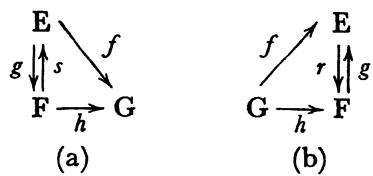
\includegraphics[keepaspectratio]{images/part001_ef8e01c05a3dcb28772fb1963be4c012627d42ff76089463ce60c193ac31650a.jpg}}

\begin{enumerate}
\def\labelenumi{(\alph{enumi})}
\setcounter{enumi}{1}
\item
  Let E, F, G be sets, let g be an injection of F into E, and let f be a mapping of G into E. Then there exists a mapping h of G into F such that \(f = g \circ h\) if and only if \(f(\mathbf{G}) \subset f(\mathbf{F})\) . The mapping h is uniquely determined by f; if r is a retraction of g, we have \(h = r \circ f\) .
\item
  If \(f = h \circ g\) , the relation \(g(x) = g(y)\) (where \(x \in \mathbf{E}\) , \(y \in \mathbf{E}\) ) clearly implies \(f(x) = f(y)\) . And for every section \(s\) of \(g\) we have
\end{enumerate}

\[
h = h \circ (g \circ s) = f \circ s,
\]

which shows that h is uniquely determined by f.~Conversely, suppose that the relation \(g(x) = g(y)\) implies \(f(x) = f(y)\) ; let s be a section of \(g\) , and let \(h = f \circ s\) ; then for every \(x \in \mathbf{E}\) we have \(g(s(g(x))) = g(x)\) , hence \(f(s(g(x))) = f(x)\) , that is, \(h(g(x)) = f(x)\) and therefore \(f = h \circ g\) .

\begin{enumerate}
\def\labelenumi{(\alph{enumi})}
\setcounter{enumi}{1}
\tightlist
\item
  If \(f = g \circ h\) , then clearly \(f(\mathbf{G}) \subset f(\mathbf{F})\) , and for every retraction \(r\) of \(g\) we have \(h = (r \circ g) \circ h = r \circ f\) , which shows that \(h\) is uniquely determined by \(f\) . Conversely, suppose that \(f(\mathbf{G}) \subset f(\mathbf{F})\) ; let \(r\) be a retraction of \(g\) , and put \(h = r \circ f\) ; for every \(x \in \mathbf{G}\) , there exists \(y \in \mathbf{F}\) such that \(f(x) = g(y)\) , so that
\end{enumerate}

\[
g (h (x)) = g (r (f (x))) = g (r (g (y))) = g (y) = f (x)
\]

and therefore \(f = g \circ h\) .

\subsection{FUNCTIONS OF TWO ARGUMENTS}

A function of two arguments is a function whose domain is a set of ordered pairs (or, equivalently, a subset of a product). Let \(f\) be such a function; if \((x, y)\) is an element of the domain of \(f\) , the value \(f((x, y))\) of \(f\) at the element \((x, y)\) is generally denoted by \(f(x, y)\) . Let \(f\) be a function of two arguments, \(D\) its domain, and \(C\) its target. For each \(y\) let \(A_y\) be the set of all \(x\) such that \((x, y) \in D\) (that is, the section of \(\overline{D}^1\) at \(y\) (no. 1)). The mapping

\[
x \rightarrow f (x, y) \quad (x \in \mathrm{A} _ {y}, f (x, y) \in \mathrm{C})
\]

is called the partial mapping defined by \(f\) , with respect to the value \(y\) of the second argument, and is denoted by \(f(\bullet, y)\) , or \(f(., y)\) (or sometimes \(f_y\) ); we have \(f(\bullet, y)(x) = f(x, y)\) for all \((x, y) \in D\) . Similarly, for each \(x\) let \(B_x\) be the set of all \(y\) such that \((x, y) \in D\) . The mapping

\[
y \rightarrow f (x, y) \quad (y \in \mathbf {B} _ {x}, f (x, y) \in \mathbf {C})
\]

is called the partial mapping defined by \(f\) , with respect to the value \(x\) of the first argument, and is denoted by \(f(x, \bullet)\) , or \(f(x, \cdot)\) (or sometimes \(f_x\) ); we have \(f(x, \bullet)(y) = f(x, y)\) for all \((x, y) \in \mathbf{D}\) . If for every \(y\) (resp. \(x\) ) the partial mapping \(f(\bullet, y)\) (resp. \(f(x, \bullet)\) ) is a constant mapping, we say that \(f\) does not depend on its first (resp. second) argument; this means therefore that \(f(x, y) = f(x', y)\) whenever \((x, y)\) and \((x', y)\) belong to \(\mathbf{D}\) (resp. \(f(x, y) = f(x, y')\) whenever \((x, y)\) and \((x, y')\) belong to \(\mathbf{D}\) ). For each \(y\) belonging to the second projection of \(\mathbf{D}\) let \(g(y)\) denote the common value of the \(f(x, y)\) for \(x \in A_y\) ; the mapping \(y \to g(y)\) is then a mapping of \(\mathrm{pr}_2\mathbf{D}\) into \(\mathbf{C}\) such that

\[
g (y) = f (x, y) \quad \text {   for   all   } (x, y) \in D.
\]

Conversely, let \(g\) be a mapping of a set \(B\) into a set \(C\) , and let \(A\) be any set. Then the mapping \((x, y) \to g(y)\) of \(A \times B\) into \(C\) does not depend on its first argument.

Let \(u\) be a mapping of A into C and \(v\) a mapping of B into D. The mapping \(z \to (u(\mathrm{pr}_1z), v(\mathrm{pr}_2z))\) of \(A \times B\) into \(C \times D\) is called the (canonical) extension of \(u\) and \(v\) to the product sets, or simply the product of \(u\) and \(v\) (if there is no risk of confusion); its range is \(u\langle A\rangle \times v\langle B\rangle\) . It is denoted by \(u \times v\) . If \(u\) and \(v\) are injective (resp. surjective) then \(u \times v\) is injective (resp. surjective). If \(u\) and \(v\) are bijective, then \(u \times v\) is bijective, and its inverse mapping is \(\overline{u}^1 \times \overline{v}^1\) . If \(u'\) is a mapping of C into a set E and if \(v'\) is a mapping of D into a set F, we have

\[
\left(u ^ {\prime} \times v ^ {\prime}\right) \circ (u \times v) = \left(u ^ {\prime} \circ u\right) \times \left(v ^ {\prime} \circ v\right).
\]

If U, V are the graphs of u, v respectively, the graph W of \(u \times v\) is the set of ordered pairs \(((x, y), (z, t))\) of \((\mathbf{A} \times \mathbf{B}) \times (\mathbf{C} \times \mathbf{D})\) such that \((x, z) \in \mathbf{U}\) and \((y, t) \in \mathbf{V}\) ; the mapping \(((x, y), (z, t)) \to ((x, z), (y, t))\) puts W in one-to-one correspondence with the product \(U \times V\) (a subset of \((\mathbf{A} \times \mathbf{C}) \times (\mathbf{B} \times \mathbf{D})\) ) (cf.~§5, no. 5).

\section{UNION AND INTERSECTION OF A FAMILY OF SETS}

\subsection{DEFINITION OF THE UNION AND THE INTERSECTION OF A FAMILY OF SETS}

Let X be a family (§3, no. 4) and I its index set. To help the intuitive interpretation of what follows, we shall refer to X as a family of sets. If (X, I, G) is a family of subsets of a set E (that is, a family whose target G is such that the relation Y ∈ G implies Y ⊂ E), we shall denote the family by (X\_t)\_\{t ∈ I\}(X\_t ∈ G) or simply by (X\_t)\_\{t ∈ I\} (§3, no. 6); by abuse of notation we shall denote any family of sets, which has I as its index set, by (X\_t)\_\{t ∈ I\}.

Since the relation \((\forall x)((\iota \in I\) and \(x\in X_{\iota})\Longrightarrow (x\in X_{\iota}))\) is true, it follows from S5 (Chapter I, §4, no 2.) that the relation

\[
(\forall \iota) (\exists Z) (\forall x) ((\iota \in I \text { and } x \in X _ {\iota}) \Longrightarrow (x \in Z))
\]

is true. By virtue of the scheme S8 (§1, no. 6) the relation \((\exists t)(t \in I\) and \(x \in X_t)\) is collectivizing in \(x\) .

DEFINITION 1. Let \((\mathbf{X}_i)_{i\in I}\) be a family of sets (resp. a family of subsets of a set E). The set \(\mathcal{E}_x((\exists i)(i\in I\) and \(x\in \mathbf{X}_i))\) , that is to say, the set of all \(x\) which belong to at least one set of the family \((\mathbf{X}_{\iota})_{\iota \in \mathbf{I}}\) , is called the union of the family, and is denoted by \(\bigcup \mathbf{X}_{\iota}(*)\) .

If \((\mathbf{X}_t)_{i\in I}\) is a family of subsets of a set \(E\) , then its union is a subset of \(E\) ; notice that it does not depend on \(E\) , nor on the target \(\mathfrak{G}\) of the mapping \(t\to X_t\) .

It is clear that if \(\mathbf{I} = \emptyset\) , we have \(\bigcup_{i \in \mathbf{I}} \mathbf{X}_i = \emptyset\) , because the relation \((\exists i)(i \in \mathbf{I}\) and \(x \in \mathbf{X}_i)\) is then false.

Suppose now that \(I \neq \varnothing\) . If \(\alpha\) is an element of I, the relation

\[
(\forall \iota) ((\iota \in I) \Longrightarrow (x \in X _ {\iota}))
\]

implies \(x \in \mathbf{X}_{\alpha}\) and therefore, by virtue of C52 (§1, no. 6), this relation is collectivizing in \(x\) .

DEFINITION 2. Let \((\mathbf{X}_{\iota})_{\iota \in \mathbf{I}}\) be a family of sets whose index set I is not empty. The set \(\mathcal{E}_x((\forall \iota)((\iota \in \mathbf{I}) \Longrightarrow (x \in \mathbf{X}_{\iota}))\) , that is to say, the set of all \(x\) which belong to every set of the family \((\mathbf{X}_{\iota})_{\iota \in \mathbf{I}}\) , is called the intersection of the family and is denoted by \(\bigcap_{\iota} \mathbf{X}_{\iota}\) .

If \(I = \varnothing\) , the relation \((\forall t)((t \in I) \Longrightarrow (x \in X_t))\) is not collectivizing in \(x\) ; for it is a true relation and there exists no set \(Y\) such that \(x \in Y\) is a true relation, because \(Y\) would then be the set of all objects (cf.~§1, no. 7, Remark).

If \((\mathbf{X}_t)_{t \in \mathbf{I}}\) is a family of subsets of a set \(E\) and if \(I \neq \emptyset\) , the relation '' \(x \in E\) and \((\forall t)((t \in I) \Longrightarrow (x \in X_t))\) is equivalent to

\[
(\forall \iota) ((\iota \in I) \Longrightarrow (x \in X _ {\iota}));
\]

consequently it is collectivizing in \(x\) , and the set of all \(x\) which satisfy this relation is equal to \(\bigcap_{i \in I} X_i\) . If \(I = \emptyset\) , the relation `` \(x \in E\) and \((\forall i)((i \in I) \Longrightarrow (x \in X_i))\) '' is equivalent to \(x \in E\) ; it is therefore collectivizing in \(x\) , and the set of all \(x\) which satisfy this relation is \(E\) . Hence we may state the following definition:

DEFINITION 3. Let \((\mathbf{X}_{\iota})_{\iota \in \mathbf{I}}\) be a family of subsets of a set E. The set

\[
\mathcal {E} _ {x} (x \in \mathrm{E} \text {   and   } (\forall \iota) ((\iota \in \mathrm{I}) \Longrightarrow (x \in \mathrm{X} _ {\iota}))),
\]

in other words, the set of all \(x\) which belong to \(\mathbf{E}\) and to each of the sets \(\mathbf{X}_t\) , is called the intersection of the family and is denoted by \(\bigcap_{i=1}^{\infty} \mathbf{X}_t\) .

Hence for a family \((\mathbf{X}_{i})_{i\in\theta}\) of subsets of E we have

\[
\bigcap_ {i \in \theta} X _ {i} = E.
\]

But for a family \((\mathbf{X}_t)_{i\in I}\) of subsets of E whose index set is not empty, the intersection \(\bigcap_{i\in I}\mathbf{X}_t\) depends neither on E nor on the target of \(\iota \to \mathbf{X}_t\) ; and this justifies the use of the same notation in Definitions 2 and 3.

PROPOSITION 1. Let \((\mathbf{X}_{\mathfrak{t}})_{\mathfrak{t}\in \mathbf{I}}\) be a family of sets, and let \(f\) be a mapping of a set K onto I. Then

\[
\bigcup_ {x \in \mathbf {K}} X _ {f (x)} = \bigcup_ {i \in I} X _ {i},
\]

and, if \(\mathbf{I} \neq \emptyset\) ,

\[
\bigcap_ {x \in K} X _ {f (x)} = \bigcap_ {i \in I} X _ {i}.
\]

Let \(x\) be an element of \(\bigcap_{i \in I} X_i\) . There exists an index \(i \in I\) such that \(x \in X_i\) . Since \(f\langle K \rangle = I\) , there exists an index \(x \in K\) such that \(i = f(x)\) , whence \(x \in X_{f(x)}\) and consequently

\[
x \in \bigcup_ {x \in \mathbf {K}} X _ {f (x)}.
\]

Conversely, if \(x \in \bigcup_{x \in \mathbb{K}} X_{f(x)}\) , there exists \(x \in \mathbb{K}\) such that \(x \in X_{f(x)}\) , and therefore, since \(f(x) \in I\) , \(x \in \bigcup_{i' \in I} X_i\) . Hence

\[
\bigcup_ {x \in \mathbb {K}} X _ {f (x)} = \bigcup_ {i \in I} X _ {i}.
\]

Now suppose that \(\mathbf{I} \neq \emptyset\) , and let \(x\) be an element of \(\bigcap_{i \in \mathbf{I}} \mathbf{X}_i\) . For each element \(x\) of \(\mathbf{K}\) we have \(f(x) \in \mathbf{I}\) , hence \(x \in \mathbf{X}_{f(x)}\) , and therefore

\[
x \in \bigcap_ {x \in \mathbb {K}} X _ {f (x)}.
\]

Conversely, let \(x\) be an element of \(\bigcap_{x \in \mathbf{K}} X_{f(x)}\) . If \(\iota\) is any element of \(I\) , there exists an element \(x\) of \(K\) such that \(\iota = f(x)\) , whence \(x \in X_t\) and

consequently \(x \in \bigcap_{i \in I} X_i\) . Hence

\[
\bigcap_ {x \in \mathbf {K}} X _ {f (x)} = \bigcap_ {i \in I} X _ {i}.
\]

For families of subsets of a given set, it is clear that the second part of Proposition 1 remains valid without the restriction \(I \neq \emptyset\) .

COROLLARY. Let \((\mathbf{X}_t)_{i\in \mathbf{I}}\) be a family of sets such that \(\mathbf{X}_t = \mathbf{X}_x\) for each pair of indices \((\mathfrak{t},\mathfrak{x})\) . Then for each \(\alpha \in \mathbf{I}\) we have

\[
\bigcup_ {i \in I} X _ {i} = X _ {\alpha}, \quad \text{and} (\text{if } I \neq \varnothing) \quad \bigcap_ {i \in I} X _ {i} = X _ {\alpha}.
\]

Apply Proposition 1 to the constant mapping \(\iota\to\alpha\) of I onto \(\{\alpha\}\) .

DEFINITION 4. Let \(\mathfrak{F}\) be a set of sets and let \(\Phi\) be the family of sets defined by the identity mapping of \(\mathfrak{F}\) . The union of the sets of \(\Phi\) and (if \(\mathfrak{F}\) is not empty) the intersection of the sets of \(\Phi\) are called, respectively, the union and the intersection of the sets of \(\mathfrak{F}\) , and are denoted by \(\bigcup_{X\sim X^{\prime}}X\) and \(\bigcap_{X\sim X^{\prime}}X\) .

It follows immediately from Proposition 1 that if \((\mathbf{X}_i)_{i\in I}\) is a family of sets, then the union and (if \(I\neq \emptyset\) ) the intersection of the family are respectively equal to the union and the intersection of the sets of the set of elements of this family.

\subsection{PROPERTIES OF UNION AND INTERSECTION}

If \((\mathbf{X}_t)_{t\in \mathbf{I}}\) and \((\mathbf{Y}_t)_{t\in \mathbf{I}}\) are families of sets having the same index set \(\mathbf{I}\) , and if \(\mathbf{Y}_t\subset \mathbf{X}_t\) for each \(t\in \mathbf{I}\) , then it is clear that

\[
\bigcup_ {i \in I} Y _ {i} \subset \bigcup_ {i \in I} X _ {i}, \quad \text { and } (\text { if   } I \neq \emptyset) \quad \bigcap_ {i \in I} Y _ {i} \subset \bigcap_ {i \in I} X _ {i}.
\]

Let \((\mathbf{X}_t)_{t\in \mathbf{I}}\) be a family of sets. If \(J\subset I\) , we have

\[
\bigcup_ {i \in J} X _ {i} \subset \bigcup_ {i \in I} X _ {i}, \quad \text { and } (\text { if } J \neq \emptyset) \quad \bigcap_ {i \in J} X _ {i} \supset \bigcap_ {i \in I} X _ {i}.
\]

PROPOSITION 2. Let \((\mathbf{X}_{\iota})_{\iota \in \mathbf{I}}\) be a family of sets whose index set I is the union of a family \((\mathrm{J}_{\lambda})_{\lambda \in \mathbf{L}}\) of sets. Then

\[
\bigcup_ {i \in I} X _ {i} = \bigcup_ {\lambda \in L} \left(\bigcup_ {i \in J _ {\lambda}} X _ {i}\right),
\]

and (if \(\mathbf{L} \neq \phi\) and \(J_{\lambda} \neq \phi\) for each \(\lambda \in \mathbf{L}\) )

\[
\bigcap_ {i \in I} X _ {i} = \bigcap_ {\lambda \in L} \left(\bigcap_ {i \in J _ {\lambda}} X _ {i}\right)
\]

(``associativity'' of union and intersection).

Let \(x\) be an element of \(\bigcup_{i \in I} X_i\) . There exists an index \(i \in I\) such that \(x \in X_i\) . Since \(I\) is the union of the family \((J_\lambda)_{\lambda \in L}\) , there exists an index \(\lambda \in L\) such that \(i \in J_\lambda\) , whence \(x \in \bigcup X_i\) , and consequently

\[
x \in \bigcup_ {\lambda \in L} \left(\bigcup_ {i \in J _ {\lambda}} X _ {i}\right).
\]

Conversely, let \(x\) be an element of this set. There exists an index \(\lambda \in L\) such that \(x \in \bigcup_{\iota \in J_{\lambda}} X_{\iota}\) , hence there exists an index \(\iota \in J_{\lambda}\) (and therefore \(\iota \in I\) ) such that \(x \in X_{\iota}\) ; it follows that

\[
x \in \bigcup_ {i \in I} X _ {i}.
\]

Now suppose that \(L \neq \emptyset\) and \(J_{\lambda} \neq \emptyset\) for each \(\lambda \in L\) . Then \(I \neq \emptyset\) . Let x be an element of \(\bigcap_{i \in I} X_{i}\) . If \(\lambda \in L\) , we have \(x \in X_{i}\) for each \(i \in J_{\lambda}\) (since \(J_{\lambda} \subset I\) ), whence \(x \in \bigcap_{i \in J_{\lambda}} X_{i}\) . Since the last inclusion is true for all \(\lambda \in L\) , x belongs to \(\bigcap_{\lambda \in L} \left( \bigcap_{i \in J_{\lambda}} X_{i} \right)\) . Conversely, let x be an element of this latter set, and let i be any element of I. There exists \(\lambda \in L\) such that \(i \in J_{\lambda}\) ; since \(x \in \bigcap_{i \in J_{\lambda}} X_{i}\) , we have \(x \in X_{i}\) , which is true for all \(i \in I\) . Hence \(x \in \bigcap_{i \in I} X_{i}\) . This completes the proof.

For families of subsets of a given set the second part of Proposition 2 remains valid without restriction on L and \(J_{\lambda}\) .

\subsection{IMAGES OF A UNION AND AN INTERSECTION}

PROPOSITION 3. Let \((\mathbf{X}_t)_{t\in I}\) be a family of subsets of a set A, and let \(\Gamma\) be a correspondence between A and B. Then

\[
\Gamma \left\langle \bigcup_ {i \in I} X _ {i} \right\rangle = \bigcup_ {i \in I} \Gamma \left\langle X _ {i} \right\rangle , \quad \Gamma \left\langle \bigcap_ {i \in I} X _ {i} \right\rangle \subset \bigcap_ {i \in I} \Gamma \left\langle X _ {i} \right\rangle .
\]

The relation \((\exists x)\left(x\in \bigcup_{i\in I}X_i \text{ and } y\in \Gamma (x)\right)\) is equivalent to

\[
(\exists x) (\exists t) (t \in I \text {   and   } x \in X _ {t} \text {   and   } y \in \Gamma (x)),
\]

hence to \((\exists \iota)(\iota \in I \text{ and } y \in \Gamma\langle X_{\iota}\rangle)\) , hence is equivalent to \(y \in \bigcup_{\iota \in I} \Gamma\langle X_{\iota}\rangle\) ; this proves the first formula. As to the second formula, we have \(\bigcap_{\iota \in I} X_{\iota} \subset X_{\iota}\) for all \(\iota \in I\) , whence (§3, Proposition 2)

\[
\Gamma \left\langle \bigcap_ {i \in I} X _ {i} \right\rangle \subset \Gamma \left\langle X _ {i} \right\rangle ,
\]

and consequently

\[
\Gamma \left\langle \bigcap_ {i \in I} X _ {i} \right\rangle \subset \bigcap_ {i \in I} \Gamma \left\langle X _ {i} \right\rangle .
\]

If \(\Gamma\) is an arbitrary correspondence (and in particular an arbitrary function), the formula

\[
\Gamma \left\langle \bigcap_ {i \in I} X _ {i} \right\rangle = \bigcap_ {i \in I} \Gamma \left\langle X _ {i} \right\rangle
\]

is usually false.

* For example, in the plane \(\mathbf{R}^2\) the first projections of the lines \(y = x\) and \(y = x + 1\) are equal to \(\mathbf{R}\) , but the intersection of these lines is empty, and therefore so is the first projection of this intersection (*). *

However, we have the following important result:

PROPOSITION 4. Let \(f\) be a mapping of A into B and let \((\mathbf{Y}_t)_{t \in I}\) be a family of subsets of B. Then \(\overline{f}^1 \left\langle \bigcap_{i \in I} \mathbf{Y}_t \right\rangle = \bigcap_{i \in I} \overline{f}^1 \langle \mathbf{Y}_t \rangle\) .

To prove this, let \(x\) be an element of \(\bigcap_{i \in I} f^{-1} \langle Y_i \rangle\) . We have \(f(x) \in Y_i\) for all \(i \in I\) , whence \(f(x) \in \bigcap_{i \in I} Y_i\) , and consequently

\[
x \in \overline {{f}} ^ {1} \left\langle \bigcap_ {\iota \in I} Y _ {\iota} \right\rangle .
\]

Therefore \(\bigcap_{i\in I}\overline{f}^{1}(Y_{i})\subset\overline{f}^{1}\Big\langle\bigcap_{i\in I}Y_{i}\Big\rangle\) ; this relation, together with Proposition 3, gives the result.

COROLLARY. If \(f\) is an injection of \(A\) into \(B\) and if \((X_{t})_{t \in I}\) is a family of subsets of \(A\) whose index set \(I\) is not empty, then \(f\left\langle \bigcap_{i \in I} X_{t} \right\rangle = \bigcap_{i \in I} f\langle X_{t} \rangle\) .

For we may write \(f = i \circ g\) , where \(i\) is the canonical injection of \(f\langle \mathbf{A} \rangle\) into \(\mathbf{B}\) and \(g\) is a bijection of \(\mathbf{A}\) onto \(f\langle \mathbf{A} \rangle\) . If \(h\) denotes the inverse mapping of \(g\) , we have \(f\langle \mathbf{X} \rangle = \overline{h}^1\langle \mathbf{X} \rangle\) for every subset \(\mathbf{X}\) of \(\mathbf{A}\) , and we are therefore brought back to Proposition 4.

\subsection{COMPLEMENTS OF UNIONS AND INTERSECTIONS}

PROPOSITION 5. For every family \((\mathbf{X}_t)_{t\in I}\) of subsets of a set E, we have

\[
\mathbb {G} _ {\mathrm{E}} \left(\bigcup_ {i \in \mathrm{I}} \mathrm{X} _ {i}\right) = \bigcap_ {i \in \mathrm{I}} \left(\mathbb {G} _ {\mathrm{E}} \mathrm{X} _ {i}\right), \quad \mathbb {G} _ {\mathrm{E}} \left(\bigcap_ {i \in \mathrm{I}} \mathrm{X} _ {i}\right) = \bigcup_ {i \in \mathrm{I}} \left(\mathbb {G} _ {\mathrm{E}} \mathrm{X} _ {i}\right).
\]

Let \(x \in \complement_{\mathbf{E}} \left( \bigcup_{i \in \mathbf{I}} \mathbf{X}_i \right)\) . Then \(x \in E\) and, for every \(i \in I\) , \(x \notin \mathbf{X}_i\) , so that \(x \in \complement_{\mathbf{E}} \mathbf{X}_i\) ; consequently

\[
x \in \bigcap_ {i \in I} \left(\complement_ {E} X _ {i}\right).
\]

Conversely, let \(x\) be an element of \(\bigcap_{i \in I} (\complement_E X_i)\) ; by the definition of intersection we have \(x \in E\) . Furthermore, if we had \(x \in \bigcup_{i \in I} X_i\) , there would exist an index \(x \in I\) such that \(x \in X_x\) , which contradicts the hypothesis \(x \in \bigcap_{i \in I} (\complement_E X_i)\) ; hence

\[
x \in \mathbb {C} _ {\mathbf {E}} \left(\bigcup_ {i \in \mathbf {I}} \mathrm{X} _ {i}\right).
\]

This proves the first formula; the second one is an immediate consequence, in view of the relation \(\mathbf{G}_{\mathbf{E}}(\mathbf{G}_{\mathbf{E}}\mathbf{X})=\mathbf{X}\) for every subset X of E.

\subsection{UNION AND INTERSECTION OF TWO SETS}

If A, B are sets, we write

\[
\mathrm{A} \cup \mathrm{B} = \bigcup_ {\mathbf {X} \in \{\mathbf {A}, \mathrm{B} \}} \mathrm{X}, \quad \mathrm{A} \cap \mathrm{B} = \bigcap_ {\mathbf {X} \in \{\mathbf {A}, \mathrm{B} \}} \mathrm{X}.
\]

It is clear that A ∪ B is the set of all objects which belong either to A or to B (or possibly to both), while A ∩ B is the set of all objects which belong to both A and B. In particular, \{x, y\} = \{x\} ∪ \{y\}. Let \{x, y, z\} = \{x, y\} ∪ \{z\}. The set \{x, y, z\} is the set whose only elements are x, y, and z. Similarly we write

\[
\{x, y, z, t \} = \{x, y, z \} \cup \{t \},
\]

and so on.

If now A, B, C, D are sets, we write

\[
\begin{array}{c} \mathrm {A \cup B \cup C = \bigcup_ {\mathbf {X} \in \{\mathrm{A,B,C} \}} X, \quad A \cap B \cap C = \bigcap_ {\mathbf {X} \in \{\mathrm{A,B,C} \}} X;} \\ \mathrm {A \cup B \cup C \cup D = \bigcup_ {\mathbf {X} \in \{\mathrm{A,B,C,D} \}} X, \quad A \cap B \cap C \cap D = \bigcap_ {\mathbf {X} \in \{\mathrm{A,B,C,D} \}} X;} \end{array}
\]

and so on.

Let A, B, C be sets. From Propositions 1 and 2 we deduce the formulae

\[
\begin{array}{c} \mathbf {A} \cup \mathbf {B} = \mathbf {B} \cup \mathbf {A}, \qquad \mathbf {A} \cap \mathbf {B} = \mathbf {B} \cap \mathbf {A}, \\ \mathbf {A} \cup (\mathbf {B} \cup \mathbf {C}) = (\mathbf {A} \cup \mathbf {B}) \cup \mathbf {C} = \mathbf {A} \cup \mathbf {B} \cup \mathbf {C}, \\ \mathbf {A} \cap (\mathbf {B} \cap \mathbf {C}) = (\mathbf {A} \cap \mathbf {B}) \cap \mathbf {C} = \mathbf {A} \cap \mathbf {B} \cap \mathbf {C}. \end{array}
\]

These formulae are also immediate consequences of the theorems enunciated in the criterion C24 (Chapter I, §3, no. 5). Similarly one proves the formulae

\[
\mathbf {A} \cup (\mathbf {B} \cap \mathbf {C}) = (\mathbf {A} \cup \mathbf {B}) \cap (\mathbf {A} \cup \mathbf {C}), \quad \mathbf {A} \cap (\mathbf {B} \cup \mathbf {C}) = (\mathbf {A} \cap \mathbf {B}) \cup (\mathbf {A} \cap \mathbf {C})
\]

(``distributivity'' of union over intersection and of intersection over union; cf.~§5, no. 6).

The relation \(\mathbf{A} \subset \mathbf{B}\) is equivalent to \(\mathbf{A} \cup \mathbf{B} = \mathbf{B}\) and to \(\mathbf{A} \cap \mathbf{B} = \mathbf{A}\) . If \(\mathbf{A}\) and \(\mathbf{B}\) are subsets of a set \(\mathbf{E}\) , we deduce from Proposition 5 (or from criterion C24) the formulae

\[
\mathbb {G} _ {\mathbf {E}} (\mathbf {A} \cup \mathbf {B}) = \left(\mathbb {G} _ {\mathbf {E}} \mathbf {A}\right) \cap \left(\mathbb {G} _ {\mathbf {E}} \mathbf {B}\right), \quad \mathbb {G} _ {\mathbf {E}} (\mathbf {A} \cap \mathbf {B}) = \left(\mathbb {G} _ {\mathbf {E}} \mathbf {A}\right) \cup \left(\mathbb {G} _ {\mathbf {E}} \mathbf {B}\right);
\]

furthermore, we have

\[
\mathrm{A} \cup (\mathbb {C} _ {\mathrm{E}} \mathrm{A}) = \mathrm{E}, \quad \mathrm{A} \cap (\mathbb {C} _ {\mathrm{E}} \mathrm{A}) = \varnothing .
\]

If \(\Gamma\) is a correspondence between \(E\) and \(F\) , and if \(A, B\) are subsets of \(E\) , it follows from Proposition 3 that

\[
\Gamma \langle \mathrm{A} \cup \mathrm{B} \rangle = \Gamma \langle \mathrm{A} \rangle \cup \Gamma \langle \mathrm{B} \rangle , \quad \Gamma \langle \mathrm{A} \cap \mathrm{B} \rangle \subset \Gamma \langle \mathrm{A} \rangle \cap \Gamma \langle \mathrm{B} \rangle ,
\]

and that, if \(f\) is a mapping of \(F\) into \(E\) ,

\[
\overline {{{f}}} ^ {1} \langle \mathrm{A} \cap \mathrm{B} \rangle = \overline {{{f}}} ^ {1} \langle \mathrm{A} \rangle \cap \overline {{{f}}} ^ {1} \langle \mathrm{B} \rangle
\]

from Proposition 4.

We record also the following Proposition on complements :

PROPOSITION 6. Let \(f\) be a mapping of \(A\) into \(B\) . For every subset \(Y\) of \(B\) , we have

\[
\overline {{{f}}} ^ {1} \langle \mathrm{B} - \mathrm{Y} \rangle = \overline {{{f}}} ^ {1} \langle \mathrm{B} \rangle - \overline {{{f}}} ^ {1} \langle \mathrm{Y} \rangle .
\]

For \(x\) belongs to \(\overline{f}^1\langle \mathbf{B} - \mathbf{Y}\rangle\) if and only if \(f(x)\) belongs to \(\mathbf{B}\) but not to \(\mathbf{Y}\) , i.e., if and only if \(x\) belongs to \(\overline{f}^1\langle \mathbf{B}\rangle\) but not to \(\overline{f}^1\langle \mathbf{Y}\rangle\) .

COROLLARY. Let \(f\) be an injection of \(\mathbf{A}\) into \(\mathbf{B}\) . For every subset \(\mathbf{X}\) of \(\mathbf{A}\) , we have \(f\langle \mathbf{A} - \mathbf{X}\rangle = f\langle \mathbf{A}\rangle - f\langle \mathbf{X}\rangle\) .

Writing \(f = i \circ g\) , where \(i\) is the canonical injection of \(f\langle A\rangle\) into B, we reduce the Corollary to Proposition 6 applied to \(\overline{g}^1\) .

¶ The intersection X ∩ A is sometimes called the trace of X on A. If F is a family of sets, the set of traces on A of the sets belonging to F is called the trace of F on A.

\subsection{COVERINGS}

DEFINITION 5. A family of sets \((\mathbf{X}_t)_{t \in I}\) is said to be a covering of a set E (or to cover E) if \(\mathbf{E} \subset \bigcup_{i \in I} \mathbf{X}_t\) . If \((\mathbf{X}_t)_{t \in I}\) and \((\mathbf{Y}_x)_{x \in K}\) are coverings of E, the second of these coverings is said to be finer than the first (or to be a refinement of the first, or to refine the first) if, for each \(x \in K\) , there exists \(t \in I\) such that

\[
\mathrm{Y} _ {x} \subset \mathrm{X} _ {i}.
\]

A set of sets \(\Re\) is a covering of \(E\) if the family of sets defined by the identity mapping of \(\Re\) is a covering of \(E\) , in other words, if \(E \subset \bigcup_{X \in \mathbb{R}} X\) .

If \(\Re\) , \(\Re'\) , \(\Re''\) are three coverings of E such that \(\Re'\) refines \(\Re\) and \(\Re''\) refines \(\Re'\) , it is clear that \(\Re''\) refines \(\Re\) .

Let \((\mathbf{X}_t)_{i\in I}\) be a covering of E. If J is a subset of I such that \((\mathbf{X}_t)_{i\in J}\) is still a covering of E, then this covering clearly refines \((\mathbf{X}_t)_{i\in I}\) .

Let \((\mathbf{X}_t)_{t \in I}\) and \((\mathbf{Y}_x)_{x \in K}\) be coverings of a set \(E\) . Then the family of sets \((\mathbf{X}_t \cap \mathbf{Y}_x)_{(t,x) \in I \times K}\) is a covering of \(E\) . For if \(x \in E\) , there exist indices \(t \in I\) and \(x \in K\) such that \(x \in X_t\) and \(x \in Y_x\) , so that \(x \in X_t \cap Y_x\) . Moreover, it is clear that the covering \((\mathbf{X}_t \cap Y_x)_{(t,x) \in I \times K}\) refines each \(o\) the coverings \((\mathbf{X}_t)_{i\in \mathbf{I}}, (\mathbf{Y}_x)_{x\in \mathbf{K}}\) . Conversely, let \((\mathbf{Z}_{\lambda})_{\lambda \in \mathbf{L}}\) be a covering of \(\mathbf{E}\) which refines each of the coverings \((\mathbf{X}_t)_{i\in \mathbf{I}}, (\mathbf{Y}_x)_{x\in \mathbf{K}}\) ; if \(\lambda \in \mathbf{L}\) , then there exist indices \(i\in \mathbf{I}\) and \(x\in \mathbf{K}\) such that \(Z_{\lambda}\subset X_{i}\) and \(Z_{\lambda}\subset Y_{x}\) , so that \(Z_{\lambda}\subset X_{i}\cap Y_{x}\) ; hence the covering \((Z_{\lambda})_{\lambda \in \mathbf{L}}\) is a refinement of

\[
\left(\mathrm{X} _ {i} \cap \mathrm{Y} _ {x}\right) _ {(i, x) \in \mathrm{I} \times \mathrm{K}}.
\]

Let \((\mathbf{X}_t)_{t\in I}\) be a covering of a set A, and let \(f\) be a mapping of A onto a set B. The family \((f\langle \mathbf{X}_t\rangle)_{t\in I}\) is then a covering of B (Proposition 3), called the image under \(f\) of the covering \((\mathbf{X}_t)_{t\in I}\) . If \(g\) is a mapping of a set C into the set A, the family \((\overline{g}\langle \mathbf{X}_t\rangle)_{t\in I}\) is a covering of C, called the inverse image under \(g\) of the covering \((\mathbf{X}_t)_{t\in I}\) .

Let E and F be sets, let \((\mathbf{X}_t)_{i \in I}\) be a covering of E, and let \((\mathbf{Y}_x)_{x \in K}\) be a covering of F. The family \((\mathbf{X}_t \times \mathbf{Y}_x)_{(i,x) \in I \times K}\) is then a covering of E × F, called the product of the coverings \((\mathbf{X}_t)_{i \in I}\) of E and \((\mathbf{Y}_x)_{x \in K}\) of F.

PROPOSITION 7. (1) Let E be a set and \((\mathbf{X}_{\iota})_{\iota \in \mathbf{I}}\) a covering of E. If \(f\) and \(g\) are two functions with domain E such that \(f\) and \(g\) agree on \(\mathbf{E} \cap \mathbf{X}_{\iota}\) for each \(\iota \in \mathbf{I}\) , then \(f\) and \(g\) agree on E.

\begin{enumerate}
\def\labelenumi{(\arabic{enumi})}
\setcounter{enumi}{1}
\item
  Let \((\mathbf{X}_i)_{i \in I}\) be a family of sets and let \((f_i)_{i \in I}\) be a family of mappings with the same target F such that for each \(i \in I\) the domain of \(f_i\) is \(\mathbf{X}_i\) , and for each pair \((i, x) \in I \times I\) , \(f_i\) and \(f_x\) agree on \(\mathbf{X}_i \cap \mathbf{X}_x\) . Then there is exactly one function \(f\) with domain \(A = \bigcup_{i \in I} X_i\) and target F which extends each of the functions \(f_i (i \in I)\) .
\item
  Let \(x\) be any element of \(\mathbf{E}\) . Then there exists \(t \in I\) such that \(x \in X_t\) , whence \(f(x) = g(x)\) by hypothesis.
\item
  Let \(G_{i}\) be the graph of \(f_{i}\) and let \(G = \bigcup_{i \in I} G_{i}\) ; let us show that \(G\) is a functional graph. If \((x, y) \in G\) and \((x, y') \in G\) , there exist two indices \(i, x\) in \(I\) such that \((x, y) \in G_{i}\) and \((x, y') \in G_{x}\) . This implies \(x \in X_{i}, x \in X_{x}, y = f_{i}(x), y' = f_{x}(x)\) ; but since \(x \in X_{i} \cap X_{x}\) , we have
\end{enumerate}

\[
f _ {i} (x) = f _ {x} (x),
\]

that is to say, \(y = y'\) . The graph \(G\) has domain \(\mathrm{pr}_1 G = \bigcup_{i \in I} \mathrm{pr}_1 G_i = A\) ; the function \(f = (G, A, F)\) therefore satisfies the required conditions. Its uniqueness follows from the first part of the Proposition.

\subsection{PARTITIONS}

DEFINITION 6. Two sets A and B are said to be disjoint (or not to intersect) if \(\mathbf{A} \cap \mathbf{B} = \phi\) . If \(\mathbf{A} \cap \mathbf{B} \neq \phi\) , we say that A meets (or intersects) B. Let \((\mathbf{X}_{t})_{i \in I}\) be a family of sets. The sets of this family are said to be mutually disjoint if the conditions \(i \in I\) , \(x \in I\) , \(i \neq x\) imply \(\mathbf{X}_{t} \cap \mathbf{X}_{x} = \phi\) .

Let \(f\) be a mapping of \(\mathbf{A}\) into \(\mathbf{B}\) , and let \((\mathbf{Y}_i)_{i\in \mathbf{I}}\) be a family of mutually disjoint subsets of \(\mathbf{B}\) . Proposition 4 then shows that the sets of the family \((\overline{f}^1\langle \mathbf{Y}_i\rangle)_{i\in \mathbf{I}}\) of subsets of \(\mathbf{A}\) are mutually disjoint. On the other hand, if \((\mathbf{X}_i)_{i\in \mathbf{I}}\) is a family of mutually disjoint subsets of \(\mathbf{A}\) , the sets of the family \((f\langle \mathbf{X}_i\rangle)_{i\in \mathbf{I}}\) are not in general mutually disjoint.

PROPOSITION 8. Let \((\mathbf{X}_t)_{t \in I}\) be a family of mutually disjoint sets, and let \((f_t)_{t \in I}\) be a family of functions with the same target F such that the domain of \(f_t\) is \(\mathbf{X}_t\) for each \(t \in I\) . Then there exists exactly one function \(f\) with domain \(\bigcup_{i \in I} \mathbf{X}_t\) and target F which extends each of the functions \(f_t\) ( \(t \in I\) ).

This is a corollary of Proposition 7, since \(f_{\iota}\) and \(f_{x}\) clearly agree on \(\mathbf{X}_{\iota} \cap \mathbf{X}_{x} = \emptyset\) whenever \(\iota \neq x\) .

DEFINITION 7. A partition of a set E is a family of non-empty mutually disjoint subsets of E which covers E.

Example. For every non-empty set A, the family \((\{x\})_{x\in\mathbf{A}}\) is a partition of A.

If \((\mathbf{X}_i)_{i\in I}\) is a partition of a set \(E\) , the mapping \(\iota \to X_i\) of \(I\) onto the set \(\mathfrak{F}\) of elements \(X_i\) of the partition is bijective. Hence, if \(\mathfrak{F}\) is given, the partition is determined up to a one-to-one correspondence between index sets. Usually when we speak of a partition, it is the set of elements of the partition with which we are concerned.

\subsection{SUM OF A FAMILY OF SETS}

PROPOSITION 9. Let \((\mathbf{X}_t)_{t \in I}\) be a family of sets. Then there exists a set \(\mathbf{X}\) with the following property: \(\mathbf{X}\) is the union of a family \((\mathbf{X}_t')_{t \in I}\) of mutually disjoint sets such that for each \(t \in I\) there exists a one-to-one mapping of \(\mathbf{X}_t\) onto \(\mathbf{X}_t'\) .

Let \(A = \bigcup_{i \in I} X_i\) . If \(i \in I\) , the mapping \(x \to (x, i)\) ( \(x \in X_i\) ) is a one-to-one mapping of \(X_i\) onto a subset \(X_i'\) of \(A \times I\) . Moreover, the image of \(X_i'\) under the second coordinate function on \(A \times I\) is contained in the set \(\{i\}\) ; it follows that \(X_i' \cap X_x' = \emptyset\) whenever \(i \neq x\) . We may then take \(X = \bigcup_{i \in I} X_i'\) .

DEFINITION 8. Let \((\mathbf{X}_{\iota})_{\iota \in \mathbf{I}}\) be a family of sets. The sum of this family is the union of the family of sets \((\mathbf{X}_{\iota} \times \{\iota\})_{\iota \in \mathbf{I}}\) .

PROPOSITION 10. Let \((\mathbf{X}_t)_{t\in I}\) be a family of mutually disjoint sets. Let A be its union and S its sum. Then there exists a bijective mapping of A onto S.

For each \(t \in I\) , let \(f_{t}\) be a bijection of \(X_{t}\) onto \(X_{t} \times \{t\}\) . By virtue of Proposition 8, there exists a mapping f of A into S which extends all the mappings \(f_{t}\) . It is immediately verified that f is a bijective mapping of A onto S.

By abuse of language, a set E is said to be the sum of a family of sets \((\mathbf{X}_{t})_{t\in\mathbf{I}}\) if there exists a bijection of E onto the sum of the family, as defined in Definition 8.

Note that if \((\mathbf{X}_{t})_{i\in\mathbf{I}}\) is an arbitrary family of sets, the argument of Proposition 10 shows that there exists a mapping of the sum S onto the union A.

\section{PRODUCT OF A FAMILY OF SETS}

\subsection{THE AXIOM OF THE SET OF SUBSETS}

\[
(\forall \mathbf {X}) \operatorname{Coll} _ {\mathbf {Y}} (\mathbf {Y} \subset \mathbf {X}).
\]

This axiom means that for every set X there exists a set whose elements are all the subsets of X, namely the set \(\mathcal{E}_{\mathbf{Y}}(\mathbf{Y}\subset\mathbf{X})\) (§1, no. 4); this set is denoted by \(\mathfrak{P}(\mathbf{X})\) and is called the set of subsets of X. Clearly, if \(X\subset X'\) , we have \(\mathfrak{P}(\mathbf{X})\subset\mathfrak{P}(\mathbf{X}')\) .

Let A, B be two sets and let \(\Gamma\) be a correspondence between A and B. The function \(X \to \Gamma\langle X\rangle\) ( \(X \subset \mathfrak{P}(A)\) , \(\Gamma\langle X\rangle \in \mathfrak{P}(B)\) ) is called the canonical extension (or simply the extension) of \(\Gamma\) to sets of subsets and is denoted by \(\hat{\Gamma}\) ; it is a mapping of \(\mathfrak{P}(A)\) into \(\mathfrak{P}(B)\) . If \(\Gamma'\) is a correspondence between B and a set C, the formula \((\Gamma' \circ \Gamma)\langle X\rangle = \Gamma'\langle\Gamma\langle X\rangle\rangle\) shows that the extension of \(\Gamma' \circ \Gamma\) to sets of subsets is the mapping \(\hat{\Gamma}' \circ \hat{\Gamma}\) .

PROPOSITION 1. (1) If \(f\) is a surjection of a set \(\mathbf{E}\) onto a set \(\mathbf{F}\) , the canonical extension \(\hat{f}\) of \(f\) is a surjection of \(\mathfrak{P}(\mathbf{E})\) onto \(\mathfrak{P}(\mathbf{F})\) .

\begin{enumerate}
\def\labelenumi{(\arabic{enumi})}
\setcounter{enumi}{1}
\item
  If \(f\) is an injection of \(\mathbf{E}\) into \(\mathbf{F}\) , the canonical extension \(\hat{f}\) of \(f\) is an injection of \(\mathfrak{P}(\mathbf{E})\) into \(\mathfrak{P}(\mathbf{F})\) .
\item
  If \(s\) is a section of \(f\) , then \(f \circ s\) is the identity mapping of \(\mathbf{F}\) , hence \(\hat{f} \circ \hat{s}\) is the identity mapping of \(\mathfrak{P}(\mathbf{F})\) ; therefore \(\hat{f}\) is surjective and \(\hat{s}\) is a section of \(\hat{f}\) (§3, no. 8).
\item
  The proposition is obvious if \(\mathbf{E} = \varnothing\) , because then \(\mathfrak{P}(\mathbf{E}) = \{\varnothing\}\) . If \(\mathbf{E} \neq \varnothing\) and if \(r\) is a retraction of \(f\) , then \(r \circ f\) is the identity mapping of \(\mathbf{E}\) , so that \(\hat{r} \circ \hat{f}\) is the identity mapping of \(\mathfrak{P}(\mathbf{E})\) ; therefore \(\hat{f}\) is injective, and \(\hat{r}\) is a retraction of \(\hat{f}\) (§3, no. 8).
\end{enumerate}

\subsection{SET OF MAPPINGS OF ONE SET INTO ANOTHER}

Let E, F be sets. The graph of a mapping of E into F is a subset of \(E \times F\) . The set of elements of \(\mathfrak{P}(E \times F)\) which have the property of being graphs of mappings of E into F is therefore a subset of \(\mathfrak{P}(E \times F)\) , which is denoted by \(F^{E}\) . The set of triples \(f = (G, E, F)\) , where \(G \in F^{E}\) , is therefore the set of mappings of E into F; it is denoted by \(\mathcal{F}(E, F)\) . Clearly \(G \to (G, E, F)\) is a bijection (called the canonical bijection) of \(F^{E}\) onto \(\mathcal{F}(E, F)\) . The existence of this bijection allows us to translate immediately every proposition relating to the set \(F^{E}\) into one relating to \(\mathcal{F}(E, F)\) , and vice versa.

Let E, E', F, F' be sets. Let u be a mapping of E' into E, and let v be a mapping of F into F'. Then the function \(f \rightarrow v \circ f \circ u\) is a mapping of \(\mathcal{F}(\mathrm{E}, \mathrm{F})\) into \(\mathcal{F}(\mathrm{E}', \mathrm{F}')\) .

PROPOSITION 2. (1) If \(u\) is a surjection of \(\mathbf{E}'\) onto \(\mathbf{E}\) and \(v\) an injection of \(\mathbf{F}\) into \(\mathbf{F}'\) , then the mapping \(f \to v \circ f \circ u\) is injective.

\begin{enumerate}
\def\labelenumi{(\arabic{enumi})}
\setcounter{enumi}{1}
\tightlist
\item
  If \(u\) is an injection of \(\mathbf{E}'\) into \(\mathbf{E}\) and \(v\) a surjection of \(\mathbf{F}\) onto \(\mathbf{F}'\) , then the mapping \(f \to v \circ f \circ u\) is surjective.
\end{enumerate}

We shall assume that the sets E, E', F, F' are all non-empty, since otherwise the proposition is trivially verified.

\begin{enumerate}
\def\labelenumi{(\arabic{enumi})}
\tightlist
\item
  Let \(s\) be a section of \(u\) and let \(r\) be a retraction of \(v\) (§3, Definition 11). Then \(r \circ (v \circ f \circ u) \circ s = I_F \circ f \circ I_E = f\) , so that
\end{enumerate}

\[
f \rightarrow v \circ f \circ u
\]

is injective.

\begin{enumerate}
\def\labelenumi{(\arabic{enumi})}
\setcounter{enumi}{1}
\tightlist
\item
  Let \(r'\) be a retraction of \(u\) and let \(s'\) be a section of \(v\) . For every mapping \(f': E' \to F'\) we have \(v \circ (s' \circ f' \circ r') \circ u = f'\) , which shows that the mapping \(f \to v \circ f \circ u\) is surjective.
\end{enumerate}

COROLLARY. If \(u\) is a bijection of \(\mathbf{E}'\) onto \(\mathbf{E}\) and \(v\) is a bijection of \(\mathbf{F}\) onto \(\mathbf{F}'\) , then \(f \to v \circ f \circ u\) is bijective.

Let A, B, C be three sets and let f be a mapping of \(B \times C\) into A. For every \(y \in C\) let \(f(\bullet, y)\) be the partial mapping \(x \to f(x, y)\) of B into A (§ 3, no. 9); the function \(y \to f(\bullet, y)\) is a mapping of C into \(\mathcal{F}(B, A)\) . Conversely, for every mapping g of C into \(\mathcal{F}(B, A)\) there exists a unique mapping \(f\) of \(\mathbf{B} \times \mathbf{C}\) into \(\mathbf{A}\) such that \(g(y) = f(\bullet, y)\) for each \(y \in \mathbf{C}\) , namely the mapping \((x, y) \to (g(y))(x)\) . Hence:

PROPOSITION 3. If for every mapping \(f\) of \(\mathbf{B} \times \mathbf{C}\) into \(\mathbf{A}\) we denote by \(\tilde{f}\) the mapping \(y \to f(\bullet, y)\) of \(\mathbf{C}\) into \(\mathcal{F}(\mathbf{B}, \mathbf{A})\) , then the function \(f \to \tilde{f}\) is a bijection (called the canonical bijection) of \(\mathcal{F}(\mathbf{B} \times \mathbf{C}, \mathbf{A})\) onto \(\mathcal{F}(\mathbf{C}, \mathcal{F}(\mathbf{B}, \mathbf{A}))\) .

Similarly we define a canonical bijection of \(\mathcal{F}(\mathbf{B}\times\mathbf{C},\mathbf{A})\) onto \(\mathcal{F}(\mathbf{B},\mathcal{F}(\mathbf{C},\mathbf{A}))\) . By reason of the one-to-one correspondence between mappings and functional graphs, these bijections give rise to canonical bijections of \(\mathbf{A}^{\mathbf{B}\times\mathbf{C}}\) onto \((\mathbf{A}^{\mathbf{B}})^{\mathbf{C}}\) (resp. \((\mathbf{A}^{\mathbf{C}})^{\mathbf{B}})\) .

\subsection{DEFINITIONS OF THE PRODUCT OF A FAMILY OF SETS}

Let \((\mathbf{X}_{\iota})_{\iota \in \mathbf{I}}\) be a family of sets and let \(\mathbf{F}\) be a functional graph with domain \(\mathbf{I}\) such that \(\mathbf{F}(\iota) \in \mathbf{X}_{\iota}\) for each \(\iota \in \mathbf{I}\) . Then for each \(\iota \in \mathbf{I}\) we have \(\mathbf{F}(\iota) \in \mathbf{A} = \bigcup_{\iota \in \mathbf{I}} \mathbf{X}_{\iota}\) , and therefore \(\mathbf{F}\) is an element of \(\mathfrak{P}(\mathbf{I} \times \mathbf{A})\) . The functional graphs with the above property therefore form a subset of \(\mathfrak{P}(\mathbf{I} \times \mathbf{A})\) .

DEFINITION 1. Let \((\mathbf{X}_{\iota})_{\iota \in \mathbf{I}}\) be a family of sets. The set of functional graphs \(\mathbf{F}\) with domain I such that \(\mathrm{F}(\iota) \in \mathbf{X}_{\iota}\) for each \(\iota \in \mathbf{I}\) is called the product of the family of sets \((\mathbf{X}_{\iota})_{\iota \in \mathbf{I}}\) and is denoted by \(\prod_{\iota \in \mathbf{I}} \mathbf{X}_{\iota}\) . For each \(\iota \in \mathbf{I}\) , \(\mathbf{X}_{\iota}\) is called the factor of index \(\iota\) in the product \(\prod_{\iota \in \mathbf{I}} \mathbf{X}_{\iota}\) . The mapping \(\mathrm{F} \to \mathrm{F}(\iota)\) ( \(\mathrm{F} \in \prod_{\iota \in \mathbf{I}} \mathbf{X}_{\iota}\) , \(\mathrm{F}(\iota) \in \mathbf{X}_{\iota}\) ) is called the coordinate function (or projection) of index \(\iota\) , and is denoted by \(\operatorname{pr}_{\iota}\) .

\(F(t)\) is called the coordinate of index \(t\) (or projection of index \(t\) ) of F; the image \(pr_{t}\langle A\rangle\) of a subset A of \(\prod_{i\in I}X_{i}\) under the coordinate function of index \(t\) is called the projection of index \(t\) of A. It is easily verified that \(A\subset\prod_{i\in I}pr_{t}\langle A\rangle\) .

We shall often use the notation \((x_{i})_{i\in I}\) to denote an element of \(\prod_{i\in I}X_{i}\) (§3, no. 6).

If \(\mathbf{I} = \varnothing\) , the set \(\prod_{i\in \mathbf{I}}\mathbf{X}_i\) has only one element, namely the empty set (§3, no. 4, Example 1).

If all the factors \(X_{t}\) of the product \(\prod_{i\in I}X_{t}\) are equal to the same set E, we have \(\prod_{i\in I}X_{t}=E^{I}\) ; this follows immediately from the definitions.

If \((\mathbf{X}_t)_{t\in I}\) is an arbitrary family of sets and if \(\mathbf{E}\) is a set such that

\[
\bigcup_ {i \in I} X _ {i} \subset E,
\]

then Definition 1 shows that \(\prod_{i\in I}X_i\subset E^I\) ; there is therefore a one-to-one correspondence between \(\prod_{i\in I}X_i\) and a set of mappings of \(I\) into \(E\) (i.e., a subset of \(\mathcal{F}(I,E)\) ).

If \(\mathbf{I} = \{\alpha\}\) is a set consisting of a single element, we have

\[
\prod_ {i \in I} X _ {i} = X _ {\alpha} ^ {\{\alpha \}};
\]

the mapping \(\mathbf{F} \to \mathbf{F}(\alpha)\) is then a bijection (called canonical) of \(\prod_{i \in \{x\}} \mathbf{X}_i\) onto \(\mathbf{X}_\alpha\) .

Let A, B be sets and let \(\alpha, \beta\) be distinct objects (there exist two distinct objects, for example \(\phi\) and \(\{\phi\}\) ). Consider the graph \(\{(\alpha, A), (\beta, B)\}\) , which is clearly functional and is precisely the family \((X_{t})_{t \in [\alpha, \beta]}\) such that \(X_{\alpha} = A\) and \(X_{\beta} = B\) . For each pair \((x, y) \in A \times B\) , let \(f_{x,y}\) be the functional graph \(\{(\alpha, x), (\beta, y)\}\) . It is evident that the function \((x, y) \to f_{x,y}\) is a bijective mapping of \(A \times B\) onto \(\prod_{t \in [\alpha, \beta]} X_t\) ; the inverse of this bijection is \(g \to (g(\alpha), g(\beta))\) . These two bijections are called canonical. In what follows we shall use this one-to-one correspondence to deduce properties of the product of two sets from properties of the product of a family of sets.

Let \((\mathbf{X}_i)_{i\in I}\) be a family of sets each of which consists of a single element, say \(\mathbf{X}_i = \{a_i\}\) ; then the product \(\prod_{i\in I}\mathbf{X}_i\) is a set consisting of the single element \((a_i)_{i\in I}\) .

Let E be a set. The graphs of the constant mappings \(\iota \to x\) of I into E form a subset \(\Delta\) of the product \(\mathbf{E}^{\mathrm{I}}\) , called the diagonal. If \(\overline{x}\) denotes the graph of the mapping \(\iota \to x\) (where \(x \in \mathbf{E}\) ), the mapping \(x \to \overline{x}\) is a bijection of E onto \(\Delta\) , called the diagonal mapping.

PROPOSITION 4. Let \((\mathbf{X}_i)_{i\in I}\) be a family of sets, and let \(u\) be a bijection of a set \(K\) onto the index set \(I\) . If \(U\) is the graph of \(u\) , the mapping \(\mathbf{F} \to \mathbf{F} \circ U\) of \(\prod_{i\in I} X_i\) into \(\prod_{x\in K} X_{u(x)}\) is bijective.

Let

\[
\mathrm{A} = \bigcup_ {i \in \mathbf {I}} \mathrm{X} _ {i} = \bigcup_ {\boldsymbol {x} \in \mathbf {K}} \mathrm{X} _ {u (\boldsymbol {x})}
\]

(§4, Proposition 1). The mapping \(\mathbf{F} \to \mathbf{F} \circ \mathbf{U} (\mathbf{F} \in \mathbf{A}^{\mathbf{I}})\) is a bijection of \(\mathbf{A}^{\mathbf{I}}\) onto \(\mathbf{A}^{\mathbf{K}}\) (Proposition 2). It is evident that the condition ``for each \(\iota \in \mathbf{I}, \mathbf{F}(\iota) \in \mathbf{X}_{\iota}\) '' is equivalent to ``for each \(x \in K, (\mathbf{F} \circ \mathbf{U})(x) \in X_{u(x)}\) '', and the result follows.

\subsection{PARTIAL PRODUCTS}

Let \((\mathbf{X}_i)_{i\in I}\) be a family of sets, and let \(J\) be a subset of \(I\) . The product \(\prod_{i\in J} X_i\) is called a partial product of \(\prod_{i\in I} X_i\) . If \(f\) is a function whose graph \(F\) is a member of \(\prod_{i\in I} X_i\) , then \(F \circ \Delta_J\) (where \(\Delta_J\) is the diagonal of \(J \times J\) ) is the graph of the restriction of \(f\) to \(J\) . Clearly \(F \circ \Delta_J \in \prod_{i\in J} X_i\) ; the mapping \(F \to F \circ \Delta_J\) of \(\prod_{i\in I} X_i\) into \(\prod_{i\in I} X_i\) is called the projection of index \(J\) and is denoted by \(\operatorname{pr}_J\) .

PROPOSITION 5. Let \((\mathbf{X}_{\iota})_{\iota \in \mathbf{I}}\) be a family of sets and let \(\mathbf{J}\) be a subset of \(\mathbf{I}\) . If for each \(\iota \in \mathbf{I}\) we have \(\mathbf{X}_{\iota} \neq \emptyset\) , the projection \(\operatorname{pr}_{\mathbf{J}}\) is a mapping of \(\prod_{\iota \in \mathbf{I}} \mathbf{X}_{\iota}\) onto \(\prod_{\iota \in \mathbf{J}} \mathbf{X}_{\iota}\) .

In view of the remarks made above, it is enough to prove the following proposition :

PROPOSITION 6. Let \((\mathbf{X}_{\iota})_{\iota \in \mathbf{I}}\) be a family of sets such that \(\mathbf{X}_{\iota} \neq \emptyset\) for all \(\iota \in \mathbf{I}\) . If \(g\) is a mapping of \(\mathbf{J} \subset \mathbf{I}\) into \(\mathbf{A} = \bigcup_{\iota \in \mathbf{I}} \mathbf{X}_{\iota}\) such that \(g(\iota) \in \mathbf{X}_{\iota}\) for all \(\iota \in \mathbf{J}\) , then there exists an extension \(f\) of \(g\) to \(\mathbf{I}\) such that \(f(\iota) \in \mathbf{X}_{\iota}\) for all \(\iota \in \mathbf{I}\) .

For each \(\iota\in I-J\) let \(T_{\iota}\) denote the term \(\tau_{y}(y\in X_{\iota})\) . Since \(X_{\iota}\neq\emptyset\) by hypothesis, we have \(T_{\iota}\in X_{\iota}\) for all \(\iota\in I-J\) (Chapter I, §4, no. 1). If G is the graph of \(g\) , the graph \(G\cup\left(\bigcup_{\iota\in I-J}\{(\iota,T_{\iota})\}\right)\) is the graph of a function which has the required properties, as is immediately verified.

COROLLARY 1. Let \((\mathbf{X}_{\iota})_{\iota \in \mathbf{I}}\) be a family of sets such that for each \(\iota \in \mathbf{I}\) we have \(\mathbf{X}_{\iota} \neq \emptyset\) . Then for each \(\alpha \in \mathbf{I}\) the projection \(\operatorname{pr}_{\alpha}\) is a mapping of \(\prod_{\iota \in \mathbf{I}} \mathbf{X}_{\iota}\) onto \(\mathbf{X}_{\alpha}\) .

Apply Proposition 5 to the subset \(J = \{\alpha\}\) of I and note that \(\mathbf{pr}_{\alpha}\) is the composition of the canonical mapping of \(X_{\alpha}^{\{\alpha\}}\) onto \(X_{\alpha}\) and the mapping \(\mathbf{pr}_{\{\alpha\}}\) .

COROLLARY 2. Let \((\mathbf{X}_t)_{i \in \mathbf{I}}\) be a family of sets. Then \(\prod_{i \in \mathbf{I}} \mathbf{X}_t = \varnothing\) if and only if there exists \(i \in \mathbf{I}\) such that \(\mathbf{X}_t = \varnothing\) .

If we have \(X_{t} \neq \varnothing\) for each \(t \in I\) , then it follows from Corollary 1 that \(\prod_{i \in I} X_{t} \neq \varnothing\) ; conversely, if \(\prod_{i \in I} X_{t} \neq \varnothing\) , the relation \(\Pr_{\alpha}\left(\prod_{i \in I} X_{t}\right) \subset X_{\alpha}\) shows that \(X_{\alpha} \neq \varnothing\) for each \(\alpha \in I\) .

Hence, if we have a family \((\mathbf{X}_{t})_{t\in\mathbf{I}}\) of non-empty sets, we may introduce (as an auxiliary constant) a function f with domain I such that \(f(t)\in\mathbf{X}_{t}\) for all \(t\in I\) . In practice one says: ``take an element \(x_{t}\) in each \(X_{t}\) ''. Intuitively, we have thus ``chosen'' an element \(x_{t}\) in each set \(X_{t}\) ; the introduction of the logical sign \(\tau\) and the criteria governing its use absolve us from the necessity of formulating an ``axiom of choice'' to legalize this operation (cf.~Summary of Results, §4, no. 10).

COROLLARY 3. Let \((\mathbf{X}_t)_{i\in I}\) and \((\mathbf{Y}_t)_{i\in I}\) be two families of sets having the same index set I. If \(\mathbf{X}_t\subset \mathbf{Y}_t\) for each \(i\in I\) , then

\[
\prod_ {i \in I} X _ {i} \subset \prod_ {i \in I} Y _ {i}.
\]

Conversely, if \(\prod_{i\in I}X_i\subset \prod_{i\in I}Y_i\) , and if \(X_{i}\neq \emptyset\) for each \(i\in I\) , then \(X_{i}\subset Y_{i}\) for each \(i\in I\) .

The first assertion is obvious, and the second follows from Proposition 1, Corollary 5, because we have then, for each \(\alpha \in I\) ,

\[
\mathrm{X} _ {\alpha} = \operatorname{pr} _ {\alpha} \left(\prod_ {i \in \mathrm{I}} \mathrm{X} _ {i}\right) \subset \operatorname{pr} _ {\alpha} \left(\prod_ {i \in \mathrm{I}} \mathrm{Y} _ {i}\right) = \mathrm{Y} _ {\alpha}.
\]

\subsection{ASSOCIATIVITY OF PRODUCTS OF SETS}

PROPOSITION 7. Let \((\mathbf{X}_t)_{t \in \mathbf{I}}\) be a family of sets whose index set I is not the empty set. Let \((\mathrm{J}_{\lambda})_{\lambda \in \mathbf{L}}\) be a partition of I. Then the mapping

\[
f \rightarrow (\mathrm{pr} _ {\mathbf {J} _ {\lambda}} f) _ {\lambda \in \mathbf {L}}
\]

of \(\prod_{i\in I}X_i\) into the product set \(\prod_{\lambda \in L}\left(\prod_{i\in J_\lambda}X_i\right)\) is bijective (``associativity'' of products of sets).

From the interpretation of \(\mathbf{pr}_{\mathbf{J}_{\lambda}}f\) as the graph of the restriction of the function whose graph is \(f\) (no. 4), it follows that the statement that the mapping \(f \to (\mathbf{pr}_{\mathbf{J}_{\lambda}}f)_{\lambda \in \mathbf{L}}\) is bijective means that, for each family \((v_{\lambda})_{\lambda \in \mathbf{L}}\) , where \(v_{\lambda}\) is a mapping of \(\mathbf{J}_{\lambda}\) into \(\bigcup_{i\in I}\mathbf{X}_i\) , there exists a unique mapping \(u\)

of I into \(\bigcup_{i\in I}X_i\) such that \(v_{\lambda}\) is the restriction of \(u\) to \(J_{\lambda}\) for each \(\lambda\in L\) . But this is a consequence of the hypothesis that \((J_{\lambda})_{\lambda\in L}\) is a partition of I (§4, Proposition 8).

The bijection defined in Proposition 7, and its inverse bijection are said to be canonical.

\minorheading{Remarks}

\begin{enumerate}
\def\labelenumi{(\arabic{enumi})}
\tightlist
\item
  Let \(\alpha, \beta\) be two distinct objects and let \((J_{\lambda})_{\lambda \in \{\alpha, \beta\}}\) be a partition of I into two sets \(J_{\alpha}, J_{\beta}\) . We thus obtain a one-to-one mapping (again called canonical) of the product \(\prod_{i \in I} X_i\) onto \(\left(\prod_{i \in J_{\alpha}} X_i\right) \times \left(\prod_{i \in J_{\beta}} X_i\right)\) by forming the composition of the canonical mapping of \(\prod_{\lambda \in \{\alpha, \beta\}} \left(\prod_{i \in J_{\lambda}} X_i\right)\) onto \(\left(\prod_{i \in J_{\alpha}} X_i\right) \times \left(\prod_{i \in J_{\beta}} X_i\right)\) and the canonical mapping of \(\prod_{i \in I} X_i\) onto \(\prod_{\lambda \in \{\alpha, \beta\}} \left(\prod_{i \in J_{\lambda}} X_i\right)\) . If \(X_i\) is a set consisting of a single element for each \(i \in J_{\beta}\) , then \(\operatorname{pr}_{J_{\alpha}}\) is a bijective mapping of \(\prod_{i \in I} X_i\) onto \(\prod_{i \in J_{\beta}} X_i\) .
\end{enumerate}

\[
\iota \in J _ {\alpha}
\]

\begin{enumerate}
\def\labelenumi{(\arabic{enumi})}
\setcounter{enumi}{1}
\tightlist
\item
  Let \(\alpha, \beta, \gamma\) be three objects, no two of which are equal (three such objects exist; for example, \(\phi, \{\phi\}, \{\{\phi'\}\}\) ), and let A, B, C be sets. Consider the functional graph \(\{(\alpha, A), (\beta, B), (\gamma, C)\}\) , i.e., the family of sets \((X_{t})_{t \in \{\alpha, \beta, \gamma\}}\) such that \(X_{\alpha} = A\) , \(X_{\beta} = B\) , \(X_{\gamma} = C\) . To the partition of \(\{\alpha, \beta, \gamma\}\) formed by the two sets \(\{\alpha, \beta\}\) and \(\{\gamma\}\) there corresponds a canonical bijection of \(\prod X_{t}\) onto the product
\end{enumerate}

\(\iota \in \{\alpha, \beta, \gamma\}\)

\[
\left(\prod_ {\iota \in \{\alpha , \beta \}} \mathbf {X} _ {\iota}\right) \times \mathbf {X} _ {\gamma} ^ {\{\gamma \}},
\]

and hence a bijection (again called canonical) of \(\prod_{\iota \in \{\alpha, \beta, \gamma\}} \mathbf{X}_{\iota}\) onto \(\mathbf{A} \times \mathbf{B} \times \mathbf{C}\) ( \(\S 2\) , no. 2) which transforms each graph \(f \in \prod_{\iota \in \{\alpha, \beta, \gamma\}} \mathbf{X}_{\iota}\) into the element \((f(\alpha), f(\beta), f(\gamma))\) of \(\mathbf{A} \times \mathbf{B} \times \mathbf{C}\) . By Proposition 4 we may therefore put any two of the six sets \(\mathbf{A} \times \mathbf{B} \times \mathbf{C}\) , \(\mathbf{B} \times \mathbf{C} \times \mathbf{A}\) , \(\mathbf{C} \times \mathbf{A} \times \mathbf{B}\) , \(\mathbf{B} \times \mathbf{A} \times \mathbf{C}\) , \(\mathbf{A} \times \mathbf{C} \times \mathbf{B}\) , \(\mathbf{C} \times \mathbf{B} \times \mathbf{A}\) in one-to-one correspondence.

\subsection{DISTRIBUTIVITY FORMULAE}

PROPOSITION 8. Let \(((\mathbf{X}_{\lambda,1})_{i\in \mathbf{J}_2})_{\lambda \in \mathbf{L}}\) be a family (with index set L) of families of sets. Suppose that \(\mathbf{L}\neq \emptyset\) and that \(J_{\lambda}\neq \emptyset\) for each \(\lambda \in \mathbf{L}\) . Let

\[
\mathrm{I} = \prod_ {\lambda \in \mathrm{L}} \mathrm{J} _ {\lambda} \neq \emptyset .
\]

Then we have

\[
\begin{array}{l} \bigcup_ {\lambda \in \mathbf {L}} \Big (\bigcap_ {t \in \mathbf {J} _ {\lambda}} \mathbf {X} _ {\lambda , t} \Big) = \bigcap_ {f \in \mathbf {I}} \Big (\bigcup_ {\lambda \in \mathbf {L}} \mathbf {X} _ {\lambda , f (\lambda)} \Big), \\ \bigcap_ {\lambda \in \mathbf {L}} \Big (\bigcap_ {t \in \mathbf {J} _ {\lambda}} \mathbf {X} _ {\lambda , t} \Big) = \bigcup_ {f \in \mathbf {I}} \Big (\bigcap_ {\lambda \in \mathbf {L}} \mathbf {X} _ {\lambda , f (\lambda)} \Big) \end{array}
\]

(``distributivity'' of union over intersection, and of intersection over union).

Let \(x\) be an element of \(\bigcup_{\lambda \in L} \left( \bigcap_{i \in J_{\lambda}} X_{\lambda, i} \right)\) and let \(f\) be any element of 1. There exists an index \(\lambda\) such that \(x \in \bigcap_{i \in J_{\lambda}} X_{\lambda, i}\) ; consequently \(x \in X_{\lambda, f(\lambda)}\) and hence

\[
x \in \bigcup_ {\lambda \in \mathbf {L}} \mathrm{X} _ {\lambda , f (\lambda)}.
\]

Since this is true for each \(f \in I\) , we have

\[
x \in \bigcap_ {f \in I} \left(\bigcup_ {\lambda \in L} X _ {\lambda , f (\lambda)}\right).
\]

Conversely, let \(x\) be an object which does not belong to the set

\[
\bigcup_ {\lambda \in L} \left(\bigcap_ {i \in J _ {\lambda}} X _ {\lambda , i}\right).
\]

Then for each \(\lambda \in L\) we have \(x \notin \bigcap_{\iota \in J_{\lambda}} X_{\lambda, \iota}\) , which means that the set \(J_{\lambda}'\) of indices \(\iota \in J_{\lambda}\) such that \(x \notin X_{\lambda, \iota}\) is not empty for each \(\lambda \in L\) . By Proposition 5, Corollary 2, there exists a functional graph \(f\) with domain \(L\) such that for each \(\lambda \in L\) we have \(f(\lambda) \in J_{\lambda}'\) . Consequently \(f \in I\) and \(x \notin X_{\lambda, f(\lambda)}\) for each \(\lambda \in L\) ; hence

\[
x \notin \bigcup_ {\lambda \in \mathbf {L}} \mathrm{X} _ {\lambda , f (\lambda)}
\]

and thus

\[
x \notin \bigcap_ {f \in I} \left(\bigcup_ {\lambda \in L} X _ {\lambda , f (\lambda)}\right).
\]

This completes the proof of the first formula. The second formula follows by applying the first to the family \(\left((\mathbb{C}_{\Lambda}X_{\lambda,t})_{t\in J_{\lambda}}\right)_{\lambda \in L}\) , where A denotes the union \(\bigcap_{\lambda \in L}\left(\bigcap_{t\in J_{\lambda}}X_{\lambda}\right)\) .

COROLLARY. Let \((\mathbf{X}_i)_{t\in \mathbf{I}}\) and \((\mathbf{Y}_x)_{x\in \mathbb{K}}\) be two families of sets with non-empty index sets I, K. Then

\[
\begin{array}{l} \left(\bigcap_ {i \in I} X _ {i}\right) \cup \left(\bigcap_ {x \in K} Y _ {x}\right) = \bigcap_ {(i, x) \in I \times K} (X _ {i} \cup Y _ {x}), \\ \left(\bigcup_ {i \in I} X _ {i}\right) \cap \left(\bigcup_ {x \in K} Y _ {x}\right) = \bigcup_ {(i, x) \in I \times K} (X _ {i} \cap Y _ {x}). \end{array}
\]

Let \(\alpha, \beta\) be two distinct objects; apply the formulae of Proposition 8 (with \(L = \{\alpha, \beta\}\) , \(J_{\alpha} = I\) , \(J_{\beta} = K\) ) to the family \(((Z_{\lambda, \mu})_{\mu \in J_{\lambda}})_{\lambda \in L}\) , where \(Z_{\alpha, \iota} = X_{\iota}\) for all \(\iota \in I\) and \(Z_{\beta, x} = Y_{x}\) for each \(x \in K\) . By the existence of the canonical bijection of \(\prod_{\lambda \in L} J_{\lambda}\) onto \(I \times K\) (no. 3) and by Proposition 1 of §4 we obtain the formulae stated.

PROPOSITION 9. Let \(((\mathbf{X}_{\lambda, t})_{t \in \mathbf{J}_{\lambda}})_{\lambda \in \mathbf{L}}\) be a family (with index set L) of families of sets. Let \(\mathbf{I} = \prod_{\lambda \in \mathbf{J}_{\lambda}} \mathbf{J}_{\lambda}\) . Then

\[
\prod_ {\lambda \in L} \left(\bigcup_ {i \in J _ {\lambda}} X _ {\lambda , i}\right) = \bigcup_ {f \in I} \left(\prod_ {\lambda \in L} X _ {\lambda , f (\lambda)}\right)
\]

and (if \(\mathbf{L} \neq \phi\) and \(\mathbf{J}_{\lambda} \neq \phi\) for each \(\lambda \in \mathbf{L}\) )

\[
\prod_ {\lambda \in \mathrm{L}} \left(\bigcap_ {i \in \mathrm{J} _ {\lambda}} \mathrm{X} _ {\lambda , i}\right) = \bigcap_ {f \in \mathrm{I}} \left(\prod_ {\lambda \in \mathrm{L}} \mathrm{X} _ {\lambda , f (\lambda)}\right)
\]

(``distributivity'' of product over union and over intersection).

The first formula is trivially true if \(L = \emptyset\) or if \(J_{\lambda} = \emptyset\) for some \(\lambda \in L\) . If not, let \(g\) be an element of \(\prod_{\lambda \in L} \left( \bigcap_{t \in J_{\lambda}} X_{\lambda, t} \right)\) . For each \(\lambda \in L\) there exists an index \(t \in J_{\lambda}\) such that \(g(\lambda) \in X_{\lambda, t}\) ; in other words, the set \(H_{\lambda}\) of indices \(t \in J_{\lambda}\) such that \(g(\lambda) \in X_{\lambda, t}\) is not empty. By Corollary 2 to Proposition 5 there is therefore a functional graph \(f\) with domain \(L\) such that

\[
f (\lambda) \in \mathrm{H} _ {\lambda}
\]

for each \(\lambda \in L\) , i.e., \(g(\lambda) \in X_{\lambda, f(\lambda)}\) . Hence we have \(g \in \prod_{\lambda \in L} X_{\lambda, f(\lambda)}\) and consequently \(g \in \bigcup_{f \in I} \left( \prod_{\lambda \in L} X_{\lambda, f(\lambda)} \right)\) . Conversely, if

\[
g \in \bigcup_ {f \in \mathbf {I}} \left(\prod_ {\lambda \in \mathbf {L}} \mathrm{X} _ {\lambda , f (\lambda)}\right),
\]

there is a functional graph \(f \in I\) such that for every \(\lambda \in L\) we have

\[
g (\lambda) \in \mathbf {X} _ {\lambda , f (\lambda)}
\]

and, a fortiori, \(g(\lambda) \in \bigcup_{t \in J_1} X_{\lambda,t}\) . This completes the proof of the first formula. The proof of the second formula is analogous but simpler, and we leave it to the reader.

COROLLARY 1. Suppose that \(\mathbf{L} \neq \emptyset\) and that \(J_{\lambda} \neq \emptyset\) for each \(\lambda \in L\) . If for \(e\) achindex \(\lambda \in L\) the family \((X_{\lambda, t})_{t \in J_{\lambda}}\) is a partition of \(X_{\lambda} = \bigcup_{t \in J_{\lambda}} X_{\lambda, t}\) , then the family \(\left( \prod_{\lambda \in L} X_{\lambda, f(\lambda)} \right)_{f \in I}\) is a partition of \(\prod_{\lambda \in L} X_{\lambda}\) .

If we set

\[
\mathrm{P} _ {f} = \prod_ {\lambda \in \mathbf {L}} \mathrm{X} _ {\lambda , f (\lambda)},
\]

then, by virtue of the first formula of Proposition 9, it is sufficient to show that \(\mathbf{P}_f \neq \emptyset\) for all \(f \in \mathbf{I}\) and that \(\mathbf{P}_f \cap \mathbf{P}_g = \emptyset\) whenever \(f\) and \(g\) are distinct elements of \(\mathbf{I}\) . The first point follows from Proposition 5, Corollary 2. As to the second, if \(f \neq g\) , there exists \(\lambda \in \mathbf{L}\) such that

\[
f (\lambda) \neq g (\lambda)
\]

and therefore, by virtue of the hypothesis, \(\mathbf{X}_{\lambda,f(\lambda)} \cap \mathbf{X}_{\lambda,g(\lambda)} = \varnothing\) . It follows that there is no graph belonging to \(P_{f} \cap P_{g}\) ; for if G were such a graph, we would have \(\mathbf{G}(\lambda) \in \mathbf{X}_{\lambda,f(\lambda)} \cap \mathbf{X}_{\lambda,g(\lambda)} = \varnothing\) , which is absurd.

COROLLARY 2. Let \((\mathbf{X}_i)_{i\in \mathbf{I}}\) and \((\mathbf{Y}_x)_{x\in \mathbb{K}}\) be two families of sets. Then

\[
\left(\bigcup_ {i \in I} X _ {i}\right) \times \left(\bigcup_ {x \in K} Y _ {x}\right) = \bigcup_ {(i, x) \in I \times K} (X _ {i} \times Y _ {x})
\]

and, if I and K are non-empty,

\[
\left(\bigcap_ {i \in I} X _ {i}\right) \times \left(\bigcap_ {x \in K} Y _ {x}\right) = \bigcap_ {(i, x) \in I \times K} (X _ {i} \times Y _ {x}).
\]

The proof follows the pattern of the proof of the Corollary to Proposition 8.

PROPOSITION 10. Let \((\mathbf{X}_{t,x})_{(t,x)\in \mathbf{I}\times \mathbf{K}}\) be a family of sets whose index set is the product of two sets I and K. If \(\mathbf{K}\neq \emptyset\) , we have

\[
\bigcap_ {x \in \mathbf {K}} \left(\prod_ {i \in I} X _ {i, x}\right) = \prod_ {i \in I} \left(\bigcap_ {\mathbf {K} \in x} X _ {i, x}\right).
\]

Both sides of the equality to be proved are functional graphs. A graph \(f\) belongs to the left-hand side if and only if, for each \(x \in \mathbf{K}\) , \(f \in \prod_{i \in I} X_{i,x}\) ; that is, if and only if \(f(t) \in X_{t,x}\) for all \((t,x) \in I \times K\) . For \(f\) to belong to the right-hand side it is necessary and sufficient that \(f(t) \in \bigcap_{x \in K} X_{t,x}\) for each \(t \in I\) , i.e., that \(f(t) \in X_{t,x}\) for each pair \((t, x) \in I \times K\) . This completes the proof.

COROLLARY. Let \((\mathbf{X}_t)_{t\in \mathbf{I}}\) and \((\mathbf{Y}_t)_{t\in \mathbf{I}}\) be two families of sets with the same index set \(\mathbf{I}\neq \emptyset\) . Then

\[
\begin{array}{l} \left(\prod_ {i \in I} X _ {i}\right) \cap \left(\prod_ {i \in I} Y _ {i}\right) = \prod_ {i \in I} (X _ {i} \cap Y _ {i}), \\ \left(\bigcap_ {i \in I} X _ {i}\right) \times \left(\bigcap_ {i \in I} Y _ {i}\right) = \bigcap_ {i \in I} (X _ {i} \times Y _ {i}). \end{array}
\]

Apply Proposition 10 to the case where K (resp. I) is a set consisting of two distinct elements.

\subsection{EXTENSION OF MAPPINGS TO PRODUCTS}

DEFINITION 2. Let \((\mathbf{X}_t)_{t \in I}, (\mathbf{Y}_t)_{t \in I}\) be two families of sets, and let \((g_t)_{t \in I}\) be a family of functions with the same index set I such that \(g_t\) is a mapping of \(\mathbf{X}_t\) into \(\mathbf{Y}_t\) for each \(t \in I\) . For each \(f \in \prod_{t \in I} \mathbf{X}_t\) let \(u_f\) be the graph of the function \(t = g_t(f(t))\) ( \(t \in I\) ), which is an element of \(\prod_{t \in I} \mathbf{Y}_t\) . The mapping \(f \to u_f\) of \(\prod_{t \in I} \mathbf{X}_t\) into \(\prod_{t \in I} \mathbf{Y}_t\) is called the canonical extension (or simply the extension) to products of the family of mappings \((g_t)_{t \in I}\) ; it is also sometimes called the product of the family of mappings \((g_t)_{t \in I}\) .

When the index notation is used, the product of the family \((g_{i})_{i\in I}\) is the function \((x_{i})_{i\in I}\to (g_{i}(x_{i}))_{i\in I}\) ; it is sometimes denoted by \((g_{i})_{i\in I}\) .

If \(\mathbf{I} = \{\alpha, \beta\}\) , where \(\alpha\) and \(\beta\) are distinct, the extension to products of the family of mappings \((g_t)_{t \in \mathbf{I}}\) is just \(\psi \circ (g_\alpha \times g_\beta) \circ \varphi\) , where \(\varphi\) denotes the canonical mapping of \(\prod_{i \in \mathbf{I}} \mathbf{X}_i\) onto \(\mathbf{X}_\alpha \times \mathbf{X}_\beta\) (no. 3) and \(\psi\) the canonical mapping of \(\mathbf{Y}_\alpha \times \mathbf{Y}_\beta\) onto \(\prod_{i \in \mathbf{I}} \mathbf{Y}_i\) .

PROPOSITION 11. Let \((\mathbf{X}_t)_{t \in I}, (\mathbf{Y}_t)_{t \in I}, (\mathbf{Z}_t)_{t \in I}\) be three families of sets and let \((g_t)_{t \in I}, (g_t')_{t \in I}\) be two families of functions, all having the same index set, such that \(g_t\) is a mapping of \(\mathbf{X}_t\) into \(\mathbf{Y}_t\) and \(g_t'\) a mapping of \(\mathbf{Y}_t\) into \(\mathbf{Z}_t\) , for each \(t \in I\) . Let \(g\) and \(g'\) be the extensions of the families \((g_t)_{t \in I}\) and \((g_t')_{t \in I}\) to products. Then the extension of the family \((g_t' \circ g_t)_{t \in I}\) to products is equal to \(g'\circ g\) .

This follows immediately from Definition 2.

COROLLARY. Let \((\mathbf{X}_i)_{i\in I}, (\mathbf{Y}_i)_{i\in I}\) be two families of sets and let \((g_i)_{i\in I}\) be a family of functions. If \(g_i\) is an injection (resp. surjection) of \(\mathbf{X}_i\) into \(\mathbf{Y}_i\) for each \(i\in I\) , then the extension \(g\) of \((g_i)_{i\in I}\) to products is an injection (resp. surjection) of \(\prod_{i\in I} \mathbf{X}_i\) into \(\prod_{i\in I} \mathbf{Y}_i\) .

\begin{enumerate}
\def\labelenumi{(\arabic{enumi})}
\item
  Let us assume that \(X_{i} \neq \emptyset\) for each \(i \in I\) ; otherwise the result is trivial. Suppose that \(g_{i}\) is injective for each \(i \in I\) , and let \(r_{i}\) be a retraction of \(g_{i}\) (§3, no. 8, Definition 11), so that \(r_{i} \circ g_{i}\) is the identity mapping of \(X_{i}\) . Let r be the extension to products of the family \((r_{i})_{i \in I}\) ; since \(r \circ g\) is the extension to products of the family of identity mappings \(I_{X_{i}}\) , \(r \circ g\) is the identity mapping of \(\prod_{i \in I} X_{i}\) and hence g is injective (§3, Proposition 8).
\item
  Suppose that \(g_{i}\) is a surjection of \(X_{i}\) onto \(Y_{i}\) for each \(i \in I\) , and let \(s_{i}\) be a section of \(g_{i}\) ( \(\S 3\) , no. 8, definition 11), so that \(g_{i} \circ s_{i}\) is the identity mapping of \(Y_{i}\) . If \(s\) is the extension to products of the family \((s_{i})_{i \in I}\) , then \(g \circ s\) is the extension to products of the family of identity mappings \(I_{Y_{i}}\) and is therefore the identity mapping of \(\prod_{i \in I} Y_{i}\) ; hence \(g\) is surjective ( \(\S 3\) , Proposition 8).
\end{enumerate}

Let \((\mathbf{X}_i)_{i\in I}\) be a family of sets, and let E be a set. For every mapping \(f\) of E into \(\prod_{i\in I} \mathbf{X}_i\) , \(\operatorname{pr}_i \circ f\) is a mapping of E into \(\mathbf{X}_i\) . If \(\overline{f}\) is the extension to products of this family of mappings, and if \(d\) is the diagonal mapping of E into \(\mathbf{E}^{\mathrm{I}}\) , then it is immediate that \(f = \overline{f} \circ d\) . Conversely, let \((f_{t})_{t \in \mathbf{I}}\) be a family of functions such that \(f_{t}\) is a mapping of E into \(\mathbf{X}_{t}\) for each \(i \in \mathbf{I}\) , and let \(\overline{f}\) be the extension to products of this family; then we have \(\mathbf{pr}_{t} \circ (\overline{f} \circ d) = f_{t}\) for each \(t \in \mathbf{I}\) . By abuse of language, the mapping \(\overline{f} \circ d\) is also written as \((f_{t})_{t \in \mathbf{I}}\) . In this way we define a one-to-one mapping of the set \(\prod_{i \in \mathbf{I}} \mathbf{X}_{t}^{\mathbf{E}}\) onto the set \(\left(\prod_{i \in \mathbf{I}} \mathbf{X}_{t}\right)^{\mathbf{E}}\) ; this mapping and its inverse are said to be canonical.

\section{EQUIVALENCE RELATIONS}

In principle, from now on we shall stop using bold-face italic letters to denote undetermined assemblies; the reader will be able to discern easily from the context the assertions which apply to undetermined letters or relations.

\subsection{DEFINITION OF AN EQUIVALENCE RELATION}

Let \(R\{x, y\}\) be a relation, x and y being distinct letters. The relation R is said to be symmetric (with respect to the letters x and y) if

\[
\mathrm{R} \{x, y \} \Longrightarrow \mathrm{R} \{y, x \}.
\]

If so, by substituting for x and y two letters \(x'\) and \(y'\) , distinct from each other and from all the letters which appear in R, and then by substituting y and x for \(x'\) and \(y'\) , respectively, we see that

\[
\mathrm{R} \left\{y, x \right\} \Longrightarrow \mathrm{R} \left\{x, y \right\}.
\]

Hence \(\mathbb{R}\{x, y\}\) and \(\mathbb{R}\{y, x\}\) are equivalent. Let \(z\) be a letter which does not appear in \(\mathbb{R}\) . The relation \(\mathbb{R}\) is said to be transitive (with respect to the letters \(x, y\) ) if we have

\[
(\mathrm{R} \{x, y \} \text {   and   } \mathrm{R} \{y, z \}) \Longrightarrow \mathrm{R} \{x, z \}.
\]

Examples. The relation x = y is symmetric and transitive. The relation \(X \subset Y\) is transitive but not symmetric. The relation \(X \cap Y = \varnothing\) is symmetric but not transitive.

If \(\mathbf{R}\{x, y\}\) is both symmetric and transitive it is said to be an equivalence relation (with respect to the letters \(x\) and \(y\) ). In this case the notation \(x \equiv y \pmod{\mathbf{R}}\) is sometimes used as a synonym of \(\mathbf{R}\{x, y\}\) ; it is read `` \(x\) is equivalent to \(y\) modulo \(\mathbf{R}\) ''. If \(\mathbf{R}\) is an equivalence relation, we have \(\mathbf{R}\{x, y\} \Longrightarrow (\mathbf{R}\{x, x\} \text{ and } \mathbf{R}\{y, y\})\) , because \(\mathbf{R}\{x, y\}\) implies \(\mathbf{R}\{y, x\}\) , and \((\mathbf{R}\{x, y\} \text{ and } \mathbf{R}\{y, x\})\) implies \((\mathbf{R}\{x, x\} \text{ and } \mathbf{R}\{y, y\})\) by virtue of the definitions.

Let \(\mathbf{R}\{x, y\}\) be a relation; it is said to be reflexive on \(\mathbf{E}\) (with respect to the letters \(x, y\) ) if the relation \(\mathbf{R}\{x, x\}\) is equivalent to \(x \in \mathbf{E}\) . If there is no possible ambiguity about \(\mathbf{E}\) , one says simply, by abuse of language, that \(\mathbf{R}\) is reflexive.

¶ An equivalence relation on E is defined to be an equivalence relation which is reflexive on E. If R\{x, y\} is an equivalence relation on E, we have R\{x, y\} \(\Longrightarrow\) ((x, y) ∈ E × E), hence R has a graph (with respect to the letters x, y). Conversely, suppose that the equivalence relation R\{x, y\} has a graph G. Observe that the relation R\{x, x\} is equivalent to the relation (∃y)R\{x, y\}; for the former implies the latter (Chapter I, §4, no. 2, scheme S5), and conversely, since R\{x, y\} implies R\{x, x\}, (∃y)R\{x, y\} implies (∃y)R\{x, x\} and therefore also R\{x, x\}. Thus R\{x, x\} is equivalent to \(x \in pr_{1}G\) , and hence R is an equivalence relation on \(pr_{1}G\) .

An equivalence on a set E is a correspondence whose source and target are both equal to E, and whose graph F is such that the relation \((x, y) \in \mathbb{F}\) is an equivalence relation on E.

\minorheading{Examples}

\begin{enumerate}
\def\labelenumi{(\arabic{enumi})}
\item
  The relation \(x = y\) is an equivalence relation which has no graph, for if it did, the first projection of this graph would be the set of all objects.
\item
  The relation ``x = y and \(x \in E\) '' is an equivalence relation on E whose graph is the diagonal of \(E \times E\) .
\item
  The relation ``there exists a bijection of X onto Y'' is an equivalence relation which has no graph (cf.~Chapter III, § 3).
\item
  The relation `` \(x \in E\) and \(y \in E\) '' is an equivalence relation on \(E\) , whose graph is \(E \times E\) .
\item
  Suppose \(\mathbf{A} \subset \mathbf{E}\) ; then the relation
\end{enumerate}

\[
(x \in \mathrm{E} - \mathrm{A} \text { and } y = x) \text { or } (x \in \mathrm{A} \text { and } y \in \mathrm{A})
\]

is an equivalence relation on E.

\begin{enumerate}
\def\labelenumi{(\arabic{enumi})}
\setcounter{enumi}{5}
\tightlist
\item
  * The relation `` \(x \in \mathbf{Z}\) and \(y \in \mathbf{Z}\) and \(x - y\) is divisible by 4'' is an equivalence relation on \(\mathbf{Z}_{*}\) .
\end{enumerate}

PROPOSITION 1. A correspondence \(\Gamma\) between X and X is an equivalence on X if and only if it satisfies the following conditions: (a) X is the domain of \(\Gamma\) ; (b) \(\Gamma = \overline{\Gamma}^1\) ; (c) \(\Gamma \circ \Gamma = \Gamma\) .

Let \(\Gamma\) be a correspondence between X and X, and let G be its graph. If \(\Gamma\) is an equivalence on X, then \((x, x) \in G\) for all \(x \in X\) ; hence X is the domain of \(\Gamma\) . The relation \((x, y) \in G\) is equivalent to \((y, x) \in G\) , hence to \((x, y) \in \overline{G}\) , so that \(G = \overline{G}\) and therefore \(\Gamma = \overline{\Gamma}\) . The relations \((x, y) \in G\) and \((y, z) \in G\) imply \((x, z) \in G\) , so that \(G \circ G \subset G\) ; conversely, \((x, y) \in G\) implies \((x, x) \in G\) and therefore \((x, y) \in G \circ G\) , so that \(G \subset G \circ G\) ; hence \(G = G \circ G\) and consequently \(\Gamma = \Gamma \circ \Gamma\) .

Conversely, suppose that conditions (a), (b), and (c) are satisfied. The relation \((x, y) \in G\) is symmetric (by (b)) and transitive (by (c)); hence it is an equivalence relation, and by (a) it is an equivalence relation on \(X\) .

\subsection{EQUIVALENCE CLASSES ; QUOTIENT SET}

Let \(f\) be a function, \(E\) its domain, \(F\) its graph. The relation `` \(x \in E\) and \(y \in E\) and \(f(x) = f(y)\) '' is an equivalence relation on \(E\) , called the equivalence relation associated with \(f\) . It is equivalent to the relation \((\exists z)((x, z) \in F \text{ and } (y, z) \in F)\) , i.e., to \((\exists z)((x, z) \in F \text{ and } (z, y) \in \overline{F})\) , and therefore its graph is \(\overline{F} \circ F\) .

We shall now show that every equivalence relation R on a set E is of this type. Let G be the graph of R. For each \(x \in E\) the (non-empty) set \(\mathrm{G}(x) \subset \mathrm{E}\) is called the equivalence class of x with respect to R; it is thus the set of all \(y \in E\) such that \(R\{x, y\}\) . Every set which can be written as \(\mathrm{G}(x)\) for some \(x \in E\) is called an equivalence class (with respect to R). An element of an equivalence class is called a representative of this class. The set of equivalence classes with respect to R (that is, the set of all objects of the form \(\mathrm{G}(x)\) for some \(x \in E\) ) is called the quotient set of E by R and is denoted by E/R. The mapping \(x \to \mathrm{G}(x)\) ( \(x \in E\) ) whose domain is E and whose target is E/R is called the canonical mapping of E onto E/R.

C55. Let R be an equivalence relation on a set E, and let p be the canonical mapping of E onto E/R. Then

\[
\mathrm{R} \left\{x, y \right\} \Longleftrightarrow (p (x) = p (y)).
\]

With the notation above, let x and y be elements of E such that

\[
(x, y) \in G.
\]

Then \(x \in E\) and \(y \in E\) ; let us show that \(G(x) = G(y)\) . Since \(y \in G(x)\) , we have (Proposition 1) \(G(y) \subset (G \circ G)(x) = G(x)\) . On the other hand, we also have \((y, x) \in G\) , whence \(G(x) \subset G(y)\) and therefore

\[
\mathbf {G} (x) = \mathbf {G} (y),
\]

i.e., \(p(x) = p(y)\) . Conversely, if \(G(x) = G(y)\) , we have \(y \in G(y) = G(x)\) , so that \((x, y) \in G\) . This completes the proof.

A section of the canonical mapping \(p\) of \(\mathbf{E}\) onto \(\mathbf{E} / \mathbf{R}\) (§ 3, no. 8, Definition 11) is called more briefly a section of \(\mathbf{E}\) (with respect to the relation \(\mathbf{R}\) ).

\minorheading{Examples}

\begin{enumerate}
\def\labelenumi{(\arabic{enumi})}
\item
  Let R be the equivalence relation `` \(x \in E\) and \(y \in E\) and \(x = y\) '' on a set E. The equivalence class of \(x \in E\) is then the set \(\{x\}\) , and the canonical mapping \(x \to \{x\}\) of E onto E/R is bijective.
\item
  Let E, F be two sets and let R be the equivalence relation on \(E \times F\) associated with the mapping \(pr_{1}\) of \(E \times F\) onto E. The equivalence classes with respect to R are the sets of the form \(\{x\} \times F\) , where \(x \in E\) ; the mapping \(x \to \{x\} \times F\) is a bijection of E onto \((\mathbf{E} \times \mathbf{F}) / R\) .
\end{enumerate}

Let R be an equivalence relation on a set E. The quotient set E/R is a subset of \(\mathfrak{P}(E)\) , and the identity mapping of E/R is a partition of E ( \(\S4\) , no. 7); for if G is the graph of R, we have \(x \in \mathrm{G}(x)\) for all \(x \in E\) , and if two equivalence classes \(\mathbf{G}(x)\) and \(\mathbf{G}(y)\) have a common element \(z\) , then \(\mathbf{R}\{x, z\}\) and \(\mathbf{R}\{y, z\}\) , so that \(\mathbf{G}(x) = \mathbf{G}(y)\) . Furthermore, the relation

\[
(\exists \mathrm{X}) (\mathrm{X} \in \mathrm{E} / \mathrm{R} \text { and } x \in \mathrm{X} \text { and } y \in \mathrm{X})
\]

is equivalent to R\{x, y\}.

\(\mathbb{J}\) Conversely, let \((X_{i})_{i\in I}\) be a partition of a set E. It is immediately verified that the relation \((\exists i)(i\in I \text{ and } x\in X_{i} \text{ and } y\in Y_{i})\) is an equivalence relation R on E; the equivalence classes with respect to R are just the sets \(X_{i}\) of the partition, and the mapping \(i\to X_{i}\) is a bijection of I onto E/R. Every subset S of E such that, for each \(i\in I\) , the set \(S\cap X_{i}\) consists of a single element is called a system of representatives (or a transversal) of the equivalence classes with respect to R. This name is also used to denote any injection of a set K into E such that the image of K under this injection is a system of representatives of the equivalence classes with respect to R; for example, any section of E with respect to R.

\subsection{RELATIONS COMPATIBLE WITH AN EQUIVALENCE RELATION}

Let \(\mathbf{R}\{x, x'\}\) be an equivalence relation and let \(\mathbf{P}\{x\}\) be a relation. The relation \(\mathbf{P}\{x\}\) is said to be compatible with the equivalence relation \(\mathbf{R}\{x, x'\}\) (with respect to \(x\) ) if we have

\[
(\mathrm{P} \{x \} \text {   and   } \mathrm{R} \{x, y \}) \Longrightarrow \mathrm{P} \{y \},
\]

where \(y\) denotes a letter which appears neither in \(P\) nor in \(R\) .

For example, it follows from C43 (Chapter I, §5), no. 1) that every relation \(\mathbf{P}\{x\}\) is compatible with the equivalence relation \(x = x'\) .

C56. Let \(R\{x, x'\}\) be an equivalence relation on a set E, and let \(P\{x\}\) be a relation which does not contain the letter \(x'\) and is compatible (with respect to x) with the equivalence relation \(R\{x, x'\}\) . Then, if t does not appear in \(P\{x\}\) , the relation `` \(t \in E/R\) and \((\exists x)(x \in t \text{ and } P\{x\})\) '' is equivalent to the relation `` \(t \in E/R\) and \((\forall x)((x \in t) \Longrightarrow P\{x\})\) ''.

Let \(t \in \mathbb{E} / \mathbb{R}\) . If there exists \(a \in t\) such that \(\mathbb{P}\{a\}\) , then for each \(x \in t\) we have \(\mathbb{R}\{a, x\}\) and hence \(\mathbb{P}\{x\}\) . Hence \((\exists x)(x \in t \text{ and } \mathbb{P}\{x\})\) implies \((\forall x)((x \in t) \Longrightarrow \mathbb{P}\{x\})\) . The converse is obvious since \(t \in \mathbb{E} / \mathbb{R}\) implies that \(t \neq \emptyset\) .

The relation

\[
t \in \mathrm{E} / \mathrm{R} \text { and } (\exists x) (x \in t \text { and } \mathrm{P} \{x \})
\]

is said to be induced by P\{x\} on passing to the quotient (with respect to x) with respect to R. If this relation is denoted by P' \{t\}, and if f is the canonical mapping of E onto E/R, then the relation

\[
y \in \mathrm{E} \text {   and   } \mathrm{P} ^ {\prime} \left\{f (y) \right\}
\]

(where \(y\) does not appear in \(P\{x\}\) ) is equivalent to ( \(y \in E\) and \(P\{y\}\) ), as is immediately verified.

\subsection{SATURATED SUBSETS}

Let \(\mathbb{R}\{x, y\}\) be an equivalence relation on a set \(\mathbf{E}\) , and let \(\mathbf{A}\) be a subset of \(\mathbf{E}\) . A is said to be saturated with respect to \(\mathbb{R}\) if the relation \(x \in \mathbf{A}\) is compatible (with respect to \(x\) ) with \(\mathbb{R}\{x, y\}\) ; or, equivalently, if for each \(x \in \mathbf{A}\) the equivalence class of \(x\) is contained in \(\mathbf{A}\) . In other words, a set is saturated with respect to \(\mathbb{R}\) if and only if it is the union of a set of equivalence classes with respect to \(\mathbb{R}\) .

Let \(f\) be the canonical mapping of \(\mathbf{E}\) onto \(\mathbf{E} / \mathbf{R}\) . If \(\mathbf{A}\) is saturated with respect to \(\mathbf{R}\) , then the equivalence class of each \(x \in \mathbf{A}\) , which is equal to \(\overline{f}^1 \langle \{f(x)\} \rangle\) , is contained in \(\mathbf{A}\) , and hence \(\overline{f}^1 \langle f\langle \mathbf{A}\rangle \rangle \subset \mathbf{A}\) ; since in any case we have \(\mathbf{A} \subset \overline{f}^1 \langle f\langle \mathbf{A}\rangle \rangle\) , it follows that \(\overline{f}^1 \langle f\langle \mathbf{A}\rangle \rangle = \mathbf{A}\) . Conversely, if \(\mathbf{A} = \overline{f}^1 \langle f\langle \mathbf{A}\rangle \rangle\) , then for every \(x \in \mathbf{A}\) the equivalence class \(\mathbf{K} = f(x)\) of \(x\) with respect to \(\mathbf{R}\) is an element of \(f\langle \mathbf{A}\rangle\) ; and since \(\mathbf{K} = \overline{f}^1 \langle \{\mathbf{K}\}\rangle\) , we have \(\mathbf{K} \subset \overline{f}^1 \langle f\langle \mathbf{A}\rangle \rangle = \mathbf{A}\) . Thus the subsets of \(\mathbf{E}\) which are saturated with respect to \(\mathbf{R}\) are precisely the subsets \(\mathbf{A}\) of \(\mathbf{E}\) such that \(\mathbf{A} = \overline{f}^1 \langle f\langle \mathbf{A}\rangle\rangle\) . Equivalently, they are the subsets of \(\mathbf{E}\) of the form \(\overline{f}^1\langle\mathbf{B}\rangle\) , where \(\mathbf{B} \subset E / R\) ; for the relation \(A = \overline{f}^1\langle B\rangle\) implies \(B = f\langle A\rangle\) , hence \(A = \overline{f}^1\langle f\langle A\rangle\rangle\) .

If \((\mathbf{X}_t)_{t\in I}\) is a family of saturated subsets of \(E\) , then the sets \(\bigcup_{t\in I} X_t\) and \(\bigcap_{t\in I} X_t\) are saturated (§4, Propositions 3 and 4). If \(A\) is a saturated subset of \(E\) , then so is \(\complement_E A\) (§4, Proposition 6).

Let A now be an arbitrary subset of E. Then the set \(\overline{f}^1\langle f\langle \mathrm{A}\rangle \rangle\) contains A and is saturated. Conversely, if \(\mathbf{A}'\) is a saturated subset of E which contains A, we have \(f\langle \mathrm{A}'\rangle \supset f\langle \mathrm{A}\rangle\) , so that

\[
\mathrm{A} ^ {\prime} = \overline {{f}} ^ {1} \langle f \langle \mathrm{A} ^ {\prime} \rangle \rangle \supset \overline {{f}} ^ {1} \langle f \langle \mathrm{A} \rangle \rangle .
\]

Hence we may say that \(\overline{f}^1\langle f\langle A\rangle \rangle\) is the ``smallest'' saturated subset of E which contains A (cf.~Chapter III); this set is called the saturation of A with respect to the relation R. It is immediately seen that the saturation of A is the union of the equivalence classes of the elements of A. If \((\mathbf{X}_{i})_{i\in I}\) is a family of subsets of E and if \(A_{i}\) is the saturation of \(X_{i}\) with respect to R, then the saturation of \(\bigcup_{i\in I}X_{i}\) is \(\bigcup_{i\in I}A_{i}\) (§4, Proposition 3).

\subsection{MAPPINGS COMPATIBLE WITH EQUIVALENCE RELATIONS}

Let R be an equivalence relation on a set E, and let f be a function with domain E. Then f is said to be compatible with the relation R if the relation \(y = f(x)\) is compatible (with respect to x) with the relation \(R\{x, x'\}\) .

It comes to the same thing to say that the restriction of \(f\) to each equivalence class is a constant mapping, in which case we say that \(f\) is constant on each equivalence class with respect to \(\mathbf{R}\) . If \(g\) is the canonical mapping of \(\mathbf{E}\) onto \(\mathbf{E} / \mathbf{R}\) , an equivalent statement is that the relation \(g(x) = g(x')\) implies \(f(x) = f(x')\) ; hence (§3, Proposition 9) we have the following criterion:

C57. Let R be an equivalence relation on a set E, and let g be the canonical mapping of E onto E/R. Then a mapping f of E into F is compatible with R if and only if f can be put in the form h o g, where h is a mapping of E/R into F. The mapping h is uniquely determined by f; if s is any section of g, we have \(h = f \circ s\) .

The mapping h is said to be induced by f on passing to the quotient with respect to R.

Let \(f\) be a mapping of a set \(\mathbf{E}\) into a set \(\mathbf{F}\) , and let \(\mathbf{A} = f\langle \mathbf{E}\rangle \subset \mathbf{F}\) . Let \(\mathbf{R}\) be the equivalence relation associated with \(f\) (no. 2); it is clear that \(f\) is compatible with \(\mathbf{R}\) . Moreover, the mapping \(h\) induced by \(f\) on passing to the quotient is an injection of \(\mathbf{E} / \mathbf{R}\) into \(\mathbf{F}\) : for if \(t, t'\) are equivalence classes with respect to \(\mathbf{R}\) such that \(h(t) = h(t')\) , we have \(f(x) = f(x')\) for all \(x \in t\) and \(x' \in t'\) , which implies \(t = t'\) by the definition of \(\mathbf{R}\) . Let \(k\) be the mapping of \(\mathbf{E} / \mathbf{R}\) onto \(\mathbf{A}\) which has the same graph as \(h\) ; then \(k\) is bijective. If \(j\) is the canonical injection of \(\mathbf{A}\) into \(\mathbf{F}\) and if \(g\) is the canonical mapping of \(\mathbf{E}\) onto \(\mathbf{E} / \mathbf{R}\) , then we may write

\[
f = j \circ k \circ g.
\]

This relation is called the canonical decomposition of \(f\) .

Let \(f\) be a mapping of a set \(E\) into a set \(F\) , let \(R\) be an equivalence relation on \(E\) , and let \(S\) be an equivalence relation on \(F\) . Let \(u\) be the canonical mapping of \(E\) onto \(E / R\) , and let \(v\) be the canonical mapping of F onto F/S. The mapping f is said to be compatible with the equivalence relations R and S if \(v \circ f\) is compatible with R; this means that the relation \(x \equiv x' \pmod{R}\) implies \(f(x) \equiv f(x') \pmod{S}\) . The mapping h of E/R into F/S induced by \(v \circ f\) on passing to the quotient with respect to R is then called the mapping induced by f on passing to the quotients with respect to R and S; it is characterized by the relation \(v \circ f = h \circ u\) .

\subsection{INVERSE IMAGE OF AN EQUIVALENCE RELATION; INDUCED EQUIVALENCE RELATION}

Let \(\varphi\) be a mapping of a set \(E\) into a set \(F\) , and let \(S\) be an equivalence relation on \(F\) . If \(u\) is the canonical mapping of \(F\) onto \(F/S\) , the equivalence relation associated with the mapping \(u \circ \varphi\) of \(E\) into \(F/S\) is called the inverse image of \(S\) under \(\varphi\) ; if \(R\) is this relation, \(R\{x, y\}\) is equivalent to \(S\{\varphi(x), \varphi(y)\}\) , and the equivalence classes with respect to \(R\) are the inverse images under \(\varphi\) of the equivalence classes with respect to \(S\) which meet \(\varphi\langle E\rangle\) .

In particular, consider an equivalence relation R on a set E, and let A be a subset of E; then the inverse image of R under the injection j of A into E is called the equivalence relation induced by R on A, and is denoted by \(R_{A}\) .

The equivalence classes with respect to \(\mathbf{R}_{\mathbf{A}}\) are the traces on \(\mathbf{A}\) of the equivalence classes with respect to \(\mathbf{R}\) which meet \(\mathbf{A}\) . The injection \(j\) is obviously compatible with the relations \(\mathbf{R}_{\mathbf{A}}\) and \(\mathbf{R}\) ; the mapping \(h\) of \(\mathbf{A} / \mathbf{R}_{\mathbf{A}}\) into \(\mathbf{E} / \mathbf{R}\) induced by \(j\) on passing to the quotient with respect to \(\mathbf{R}_{\mathbf{A}}\) and \(\mathbf{R}\) is an injective mapping of \(\mathbf{A} / \mathbf{R}_{\mathbf{A}}\) into \(\mathbf{E} / \mathbf{R}\) : for if \(f\) (resp. \(g\) ) is the canonical mapping of \(\mathbf{E}\) onto \(\mathbf{E} / \mathbf{R}\) (resp. A onto \(\mathbf{A} / \mathbf{R}_{\mathbf{A}}\) ), then the relation \(h(g(x)) = h(g(x'))\) , where \(x \in \mathbf{A}\) and \(x' \in \mathbf{A}\) , is equivalent to \(f(x) = f(x')\) and therefore to \(g(x) = g(x')\) . The image \(h\langle \mathbf{A} / \mathbf{R}_{\mathbf{A}} \rangle\) is equal to \(f\langle \mathbf{A} \rangle\) . If \(k\) is the bijective mapping of \(\mathbf{A} / \mathbf{R}_{\mathbf{A}}\) onto \(f\langle \mathbf{A} \rangle\) which has the same graph as \(h\) , then \(k\) and its inverse are said to be canonical.

\subsection{QUOTIENTS OF EQUIVALENCE RELATIONS}

Let R, S be two equivalence relations with respect to two letters x, y. We shall say that S is finer than R (or that R is coarser than S) if the relation \(S \Longrightarrow R\) is true. If R and S are equivalence relations on the same set E, the statement that S is finer than R means that the graph of S is contained in that of R, or again that every equivalence class with respect to S is contained in an equivalence class with respect to R; or, equivalently, that every equivalence class with respect to R is saturated with respect to S.

Examples

\begin{enumerate}
\def\labelenumi{(\arabic{enumi})}
\tightlist
\item
  The relation `` \(x \in E\) and \(y \in E\) and \(x = y\) '' is finer than every equivalence relation on E. The relation `` \(x \in E\) and \(y \in E\) '' is coarser than every equivalence relation on E.
\end{enumerate}

* (2) The equivalence relation `` \(x \in \mathbf{Z}\) and \(y \in \mathbf{Z}\) and \(x - y\) is divisible by 4'' is finer than the equivalence relation `` \(x \in \mathbf{Z}\) and \(y \in \mathbf{Z}\) and \(x - y\) is divisible by 2''. *

Let R and S be two equivalence relations on the same set E, such that S is finer than R. Let f and g be the canonical mappings of E onto E/R and E onto E/S respectively; then the function f is compatible with S. Let h be the function induced by f on passing to the quotient with respect to S; then h is a mapping of E/S onto E/R. The equivalence relation associated with h on E/S is called the quotient of R by S and is denoted by R/S. The relation \(x \equiv y \pmod{R}\) is equivalent to \(g(x) \equiv g(y) \pmod{R/S}\) , and the equivalence classes with respect to R/S are the images under g of the equivalence classes with respect to R. Let \(h = j \circ h_{2} \circ h_{1}\) be the canonical decomposition (no. 5) of the mapping h. Then \(h_{1}\) is the canonical mapping of E/S onto (E/S)/(R/S), j is the identity mapping of E/R, and \(h_{2}\) is a one-to-one mapping of (E/S)/(R/S) onto E/R. The mapping \(h_{2}\) and its inverse are said to be canonical.

Conversely, consider an arbitrary equivalence relation T on the set E/S, and let R be the equivalence relation on E which is the inverse image under g of the relation T (no. 6). Since the relation \(x \equiv y \pmod{R}\) is equivalent to \(g(x) \equiv g(y) \pmod{T}\) , it follows that T is equivalent to R/S.

\subsection{PRODUCT OF TWO EQUIVALENCE RELATIONS}

Let \(R\{x, y\}\) and \(R'\{x', y'\}\) be two equivalence relations. Let \(S\{u, v\}\) denote the relation

\((\exists x)(\exists y)(\exists x^{\prime})(\exists y^{\prime})(u = (x,x^{\prime})\) and \(v = (y,y^{\prime})\) and \(\mathbf{R}\{x,y\}\) and \(\mathbf{R}'\{x',y'\}\) ;

it is immediately verified that \(S\{u, v\}\) is an equivalence relation, called the product of R and \(R'\) , and denoted by \(R \times R'\) . Suppose that R is an equivalence relation on a set E and that \(R'\) is an equivalence relation on a set \(E'\) . Then the relation \(S\{u, u\}\) is equivalent to

\[
(\exists x) (\exists x ^ {\prime}) (u = (x, x ^ {\prime}) \text { and } R \{x, x \} \text { and } R ^ {\prime} \{x ^ {\prime}, x ^ {\prime} \})
\]

i.e., to \((\exists x)(\exists x')(u = (x, x')\) and \(x \in \mathbf{E}\) and \(x' \in \mathbf{E}'\) ), hence to \(u \in \mathbf{E} \times \mathbf{E}'\) . It follows that \(\mathbf{R} \times \mathbf{R}'\) is an equivalence relation on \(\mathbf{E} \times \mathbf{E}'\) . If

\[
u = (x, x ^ {\prime})
\]

is an element of \(\mathbf{E} \times \mathbf{E}'\) , the relation \(S\{u, v\}\) is equivalent to

\[
(\exists y) (\exists y ^ {\prime}) (v = (y, y ^ {\prime}) \text {   and   } \mathrm{R} \{x, y \} \text {   and   } \mathrm{R} ^ {\prime} \{x ^ {\prime}, y ^ {\prime} \});
\]

if G and \(G'\) are the graphs of R and \(R'\) , respectively, this relation is in turn equivalent to \(v \in \mathbf{G}(x) \times \mathbf{G}(x')\) . Hence every equivalence class with respect to \(R \times R'\) is the product of an equivalence class with respect to R and an equivalence class with respect to \(R'\) , and conversely.

Let \(f\) and \(f'\) be the canonical mappings of \(\mathbf{E}\) onto \(\mathbf{E}/\mathbf{R}\) and \(\mathbf{E}'\) onto \(\mathbf{E}'/\mathbf{R}'\) , respectively, and let \(f \times f'\) be the canonical extension of \(f\) and \(f'\) to the product sets (§ 3, no. 9). Then \((f \times f')(x, x') = (f(x), f'(x'))\) for all \((x, x') \in \mathbf{E} \times \mathbf{E}'\) . The inverse image under \(f \times f'\) of an element \((u, u')\) of \((\mathbf{E}/\mathbf{R}) \times (\mathbf{E}'/\mathbf{R}')\) is just the product \(u \times u'\) of the equivalence class \(u\) with respect to \(\mathbf{R}\) and the equivalence class \(u'\) with respect to \(\mathbf{R}'\) . It follows that the equivalence relation associated with \(f \times f'\) is equivalent to \(\mathbf{R} \times \mathbf{R}'\) . The mapping \(f \times f'\) can therefore be written as \(h \circ g\) , where \(g\) is the canonical mapping of \(\mathbf{E} \times \mathbf{E}'\) onto

\[
(\mathbf {E} \times \mathbf {E} ^ {\prime}) / (\mathbf {R} \times \mathbf {R} ^ {\prime})
\]

and \(h\) is a one-to-one mapping of \((\mathbf{E} \times \mathbf{E}') / (\mathbf{R} \times \mathbf{R}')\) onto

\[
(\mathbf {E} / \mathbf {R}) \times (\mathbf {E} ^ {\prime} / \mathbf {R} ^ {\prime});
\]

this mapping h and its inverse are said to be canonical.

Remark. Let \(\mathrm{P}\{x, x'\}\) be a relation in which the letters \(y, y'\) do not occur. P is said to be compatible with the equivalence relations \(\mathrm{R}\{x, y\}\) and \(\mathrm{R}'\{x', y'\}\) (with respect to \(x\) and \(x'\) ) if the relation \((\mathrm{P}\{x, x'\}\) and \(\mathrm{R}\{x, y\}\) and \(\mathrm{R}'\{x', y'\}\) ) implies \(\mathrm{P}\{y, y'\}\) . Let \(\mathrm{Q}\{u\}\) be the relation \((\exists x)(\exists x')(u = (x, x')\) and \(\mathrm{P}\{x, x'\})\) ; then it comes to the same thing to say that \(\mathrm{Q}\{u\}\) is compatible (with respect to \(u\) ) with the equivalence relation \(\mathrm{S}\{u, v\}\) , the product of R and \(\mathrm{R}'\) .

\subsection{CLASSES OF EQUIVALENT OBJECTS}

Let \(\mathbb{R}\{x, y\}\) be an equivalence relation, which need not have a graph. It is obvious that if \(x, x', y\) are three distinct letters, the relation \(\mathbb{R}\{x, x'\}\) implies `` \(\mathbb{R}\{x, y\} \Longleftrightarrow \mathbb{R}\{x', y\}\) '' and therefore also implies the relation \((\forall y)(\mathbb{R}\{x, y\} \Longleftrightarrow \mathbb{R}\{x', y\})\) . By the scheme S7 (Chapter I, § 5, no. 1), if we put \(\theta\{x\} = \tau_y(\mathbb{R}\{x, y\})\) , the relation \(\mathbb{R}\{x, x'\}\) implies

\[
\theta \{x \} = \theta \left\{x ^ {\prime} \right\}.
\]

Note, on the other hand, that by definition \(\mathbb{R}\{x, \theta\{x\}\}\) is the relation \((\exists y)(\mathbb{R}\{x, y\})\) and hence (no. 1) is equivalent to \(\mathbb{R}\{x, x\}\) . It follows that the relation \((\mathbb{R}\{x, x\}\) and \(\mathbb{R}\{x', x'\}\) and \(\theta\{x\} = \theta\{x'\})\) is equivalent to \(\mathbb{R}\{x, x'\}\) , for it implies, by S6 (Chapter I, §5, no. 1), the relation

\[
(R \{x, x \} \text {   and   } R \{x ^ {\prime}, x ^ {\prime} \} \text {   and   } (R \{x ^ {\prime}, \theta \{x \} \} \iff R \{x ^ {\prime}, \theta \{x ^ {\prime} \} \})),
\]

hence also \((\mathbb{R}\{x, \theta\{x\}\}\) and \(\mathbb{R}\{x', \theta\{x\}\})\) , and finally \(\mathbb{R}\{x, x'\}\) by transitivity and symmetry. And since, conversely, \(\mathbb{R}\{x, x'\}\) implies \(\mathbb{R}\{x, x\}\) and \(\mathbb{R}\{x', x'\}\) , the assertion is proved. The term \(\theta\{x\}\) is called the class of objects equivalent to \(x\) (with respect to the relation \(\mathbb{R}\) ). Suppose now that \(\mathbb{T}\) is a term such that the relation

\[
(\forall y) (R \{y, y \} \Longrightarrow (\exists x) (x \in T \text {   and   } R \{x, y \}))\tag{1}
\]

is true. Then the relation \((\exists x)(R\{x, x\}\) and \(z = \theta\{x\})\) is collectivizing in \(z\) . For we may suppose that \(x \in T\) implies \(R\{x, x\}\) ; it is sufficient to replace \(T\) by the set of all \(x \in T\) such that \(R\{x, x\}\) (observing that \(R\{x, y\}\) implies \(R\{x, x\}\) ). Let \(\Theta\) be the set of all objects of the form \(\theta\{x\}\) for \(x \in T\) ( \(\S 1\) , no. 6). Suppose that \(R\{y, y\}\) is true; then there exists \(x \in T\) such that \(R\{x, y\}\) and therefore \(\theta\{y\} = \theta\{x\} \in \Theta\) . The set \(\Theta\) is called the set of classes of equivalent objects with respect to \(R\) ; and for each \(x\) such that \(R\{x, x\}\) , \(\theta\{x\}\) is the unique element \(z \in \Theta\) such that \(R\{x, z\}\) .

Under the same hypothesis, let \(\mathbf{A}\{x\}\) be a term such that \(\mathbf{R}\{x,y\}\) implies \(\mathbf{A}\{x\} = \mathbf{A}\{y\}\) . Then the relation \((\exists x)(\mathbf{R}\{x,x\}\) and \(z = \mathbf{A}\{x\})\) is collectivizing in \(z\) , since \(\mathbf{R}\{x,x\}\) , being equivalent to \(\mathbf{R}\{x,\theta\{x\}\}\) , implies \(\mathbf{A}\{x\} = \mathbf{A}\{\theta\{x\}\}\) , and consequently if \(\mathbf{E}\) is the set of objects of the form \(\mathbf{A}\{t\}\) for \(t \in \Theta\) , then \(\mathbf{R}\{x,x\}\) implies \(\mathbf{A}\{x\} \in \mathbf{E}\) . If \(f\) is the function \(t \to \mathbf{A}\{t\}\) ( \(t \in \Theta\) , \(\mathbf{A}\{t\} \in \mathbf{E}\) ), then the relation \(\mathbf{R}\{x,x\}\) implies \(\mathbf{A}\{x\} = f(\theta\{x\})\) .

In particular, if R is an equivalence relation on a set F, we may take A \(\{x\}\) to be the equivalence class of x with respect to R (no. 2), and the function f is then a bijection of \(\Theta\) onto the quotient set F/R; this justifies the terminology introduced.

* Example. Let \(\mathbb{R}\{x, y\}\) be the equivalence relation ``\(x\) and \(y\) are two vector spaces of the same finite dimension over \(\mathbf{C}\)''; this relation has no graph. It satisfies condition (1) when \(\mathbf{T}\) is the set of all vector subspaces of \(\mathbf{C}^{(\mathbf{N})}\) , or when the subset \(\mathbf{T}'\) of \(\mathbf{T}\) consists of the spaces \(\mathbf{C}^n\) ( \(n \in \mathbf{N}\) ) with the conventions that \(\mathbf{C}^0\) consists of the point 0 of \(\mathbf{C}^{(\mathbf{N})}\) and that \(\mathbf{C}^n\) ( \(n > 0\) ) is the sum of the first \(n\) components of the direct sum \(\mathbf{C}^{(\mathbf{N})}\) . With this second choice we have \(\Theta = \mathbf{T}'_*\)

\startexercises

\exercisegroup

\begin{enumerate}
\def\labelenumi{\arabic{enumi}.}
\tightlist
\item
  Show that the relation
\end{enumerate}

\[
(x = y) \iff (\forall X) ((x \in X) \Longrightarrow (y \in X))
\]

is a theorem.

\begin{enumerate}
\def\labelenumi{\arabic{enumi}.}
\setcounter{enumi}{1}
\item
  Show that \(\phi \neq \{x\}\) is a theorem. Deduce that \((\exists x)(\exists y)(x \neq y)\) is a theorem.
\item
  Let A and B be two subsets of a set X. Show that the relation \(B \subset GB\) is equivalent to \(A \subset GB\) and that the relation \(GB \subset A\) is equivalent to \(CA \subset B\) .
\item
  Prove that the relation \(\mathbf{X} \subset \{x\}\) is equivalent to
\end{enumerate}

\[
" \mathrm{X} = \{x \} \text { or } \mathrm{X} = \phi^ {\prime \prime}.
\]

\begin{enumerate}
\def\labelenumi{\arabic{enumi}.}
\setcounter{enumi}{4}
\item
  Prove that \(\phi = \tau_{\mathbf{X}}(\tau_x(x \in \mathbf{X}) \notin \mathbf{X})\) .
\item
  Let \(\mathfrak{C}\) be an equalitarian theory which contains the sign \(\in\) and the following axiom:
\end{enumerate}

A1'.

\[
(\forall y) (y = \tau_ {x} ((\forall z) (z \in x \Longleftrightarrow z \in y)))
\]

(in other words, every term is equal to the set of its elements). Show that the axiom of extent A1 is a theorem in \(\mathfrak{G}\) (use the scheme S7).

\exercisegroup

\begin{enumerate}
\def\labelenumi{\arabic{enumi}.}
\tightlist
\item
  Let \(R\{x, y\}\) be a relation, the letters x and y being distinct; let z be a letter, distinct from x and y, which does not appear in
\end{enumerate}

\(R\{x, y\}\) . Show that the relation \((\exists x)(\exists y)R\{x, y\}\) is equivalent to

\((\exists z)(z\) is an ordered pair and \(R\{\mathrm{pr}_1z, \mathrm{pr}_2z\}\) )

and that the relation \((\forall x)(\forall y)R\{x, y\}\) is equivalent to

\[
(\forall z) ((z \text {   is   an   ordered   pair }) \Longrightarrow R \{\mathrm{pr} _ {1} z, \mathrm{pr} _ {2} z \}).
\]

\begin{enumerate}
\def\labelenumi{\arabic{enumi}.}
\setcounter{enumi}{1}
\tightlist
\item
  \begin{enumerate}
  \def\labelenumii{(\alph{enumii})}
  \tightlist
  \item
    Show that the relation \(\{\{x\}, \{x, y\}\} = \{\{x'\}, \{x', y'\}\}\) is equivalent to ``\(x = x'\) and \(y = y'\)''.
  \end{enumerate}
\end{enumerate}

\begin{enumerate}
\def\labelenumi{(\alph{enumi})}
\setcounter{enumi}{1}
\tightlist
\item
  Let \(C_{0}\) be the theory of sets and let \(C_{1}\) be the theory which has the same schemes and explicit axioms as \(C_{0}\) , except for axiom A3. Show that if \(C_{1}\) is not contradictory, then \(C_{0}\) is not contradictory (use (a)).
\end{enumerate}

\exercisegroup

\begin{enumerate}
\def\labelenumi{\arabic{enumi}.}
\item
  Show that the relations \(x \in y, x \subset y, x = \{y\}\) have no graph with respect to \(x\) and \(y\) .
\item
  Let \(G\) be a graph. Show that the relation \(X \subset \mathrm{pr}_1 G\) is equivalent to \(X \subset \overline{G} \langle G \langle X \rangle \rangle\) .
\item
  Let G, H be two graphs. Show that the relation \(pr_{1}H \subset pr_{1}G\) is equivalent to \(H \subset H \circ G \circ G\) . Deduce that \(G \subset G \circ G \circ G\) .
\item
  If G is a graph, show that \(\phi \circ G = G \circ \phi = \phi\) , and that \(\overline{G} \circ G = \phi\) if and only if \(G = \phi\) .
\item
  Let A, B be two sets and let G be a graph. Show that
\end{enumerate}

\[
(\mathbf {A} \times \mathbf {B}) \circ \mathbf {G} = \overline {{\mathbf {G}}} ^ {- 1} \langle \mathbf {A} \rangle \times \mathbf {B} \quad \text { and } \quad \mathbf {G} \circ (\mathbf {A} \times \mathbf {B}) = \mathbf {A} \times \mathbf {G} \langle \mathbf {B} \rangle .
\]

\begin{enumerate}
\def\labelenumi{\arabic{enumi}.}
\setcounter{enumi}{5}
\tightlist
\item
  For each graph G, let \(G'\) be the graph \(((\mathrm{pr}_{1}\mathrm{G}) \times (\mathrm{pr}_{2}\mathrm{G})) - \mathrm{G}\) . Show that
\end{enumerate}

\[
(\overline {{\mathbf {G}}}) ^ {\prime} = \overline {{\widehat {\mathbf {G}}}} ^ {\prime},
\]

and that

\[
\mathbf {G} \circ (\overline {{\mathbf {G}}}) ^ {\prime} \subset \Delta_ {\mathbf {B}} ^ {\prime}, \quad (\overline {{\mathbf {G}}}) ^ {\prime} \circ \mathbf {G} \subset \Delta_ {\mathbf {A}} ^ {\prime}
\]

if \(\mathbf{A} \supset \mathrm{pr}_1\mathbf{G}\) and \(\mathbf{B} \supset \mathrm{pr}_2\mathbf{G}\) . Show that

\[
\mathbf {G} = \left(\operatorname{pr} _ {1} \mathbf {G}\right) \times \left(\operatorname{pr} _ {2} \mathbf {G}\right)
\]

if and only if

\[
\mathbf {G} \circ \overline {{\mathbf {G}}} ^ {\prime} \circ \mathbf {G} = \varnothing .
\]

\begin{enumerate}
\def\labelenumi{\arabic{enumi}.}
\setcounter{enumi}{6}
\tightlist
\item
  A graph G is functional if and only if for each set X we have
\end{enumerate}

\[
\mathbf {G} \langle \overline {{\mathbf {G}}} ^ {- 1} \langle \mathbf {X} \rangle \rangle \subset \mathbf {X}.
\]

\begin{enumerate}
\def\labelenumi{\arabic{enumi}.}
\setcounter{enumi}{7}
\item
  Let A, B be two sets, let \(\Gamma\) be a correspondence between A and B, and let \(\Gamma'\) be a correspondence between B and A. Show that if \(\Gamma'(\Gamma(x)) = \{x\}\) for all \(x \in A\) and if \(\Gamma(\Gamma'(y)) = \{y\}\) for all \(y \in B\) , then \(\Gamma\) is a bijection of A onto B, and \(\Gamma'\) is the inverse mapping.
\item
  Let A, B, C, D be sets, f a mapping of A into B, g a mapping of B into C, h a mapping of C into D. If \(g \circ f\) and \(h \circ g\) are bijections, show that all of f, g, h are bijections.
\item
  Let A, B, C be sets, f a mapping of A into B, g a mapping of B into C, h a mapping of C into A. Show that if two of the three mappings \(h \circ g \circ f\) , \(g \circ f \circ h\) , \(f \circ h \circ g\) are surjections and the third is an injection, then f, g, h are all bijections.
\end{enumerate}

*11. Find the error in the following argument: Let \(\mathbf{N}\) denote the set of natural numbers and let \(\mathbf{A}\) denote the set of all integers \(n > 2\) for which there exist three strictly positive integers \(x, y, z\) such that \(x^n + y^n = z^n\) . Then the set \(\mathbf{A}\) is not empty (in other words, ``Fermat's last theorem'' is false). For let \(\mathbf{B} = \{\mathbf{A}\}\) and \(\mathbf{C} = \{\mathbf{N}\}\) ; \(\mathbf{B}\) and \(\mathbf{C}\) are sets consisting of a single element, hence there is a bijection \(f\) of \(\mathbf{B}\) onto \(\mathbf{C}\) . We have \(f(\mathbf{A}) = \mathbf{N}\) ; if \(\mathbf{A}\) were empty we should have \(\mathbf{N} = f(\phi) = \phi\) , which is absurd. *

\exercisegroup

\begin{enumerate}
\def\labelenumi{\arabic{enumi}.}
\tightlist
\item
  Let \(G\) be a graph. Show that the following three propositions are equivalent:
\end{enumerate}

\begin{enumerate}
\def\labelenumi{(\alph{enumi})}
\item
  \(\mathbf{G}\) is a functional graph.
\item
  If \(\mathbf{X},\mathbf{Y}\) are any two sets, then
\end{enumerate}

\[
\overline {{{\mathbf {G}}}} (\mathbf {X} \cap \mathbf {Y}) = \overline {{{\mathbf {G}}}} (\mathbf {X}) \cap \overline {{{\mathbf {G}}}} (\mathbf {Y}).
\]

\begin{enumerate}
\def\labelenumi{(\alph{enumi})}
\setcounter{enumi}{2}
\tightlist
\item
  The relation \(\mathbf{X} \cap \mathbf{Y} = \varnothing\) implies
\end{enumerate}

\[
\overline {{\mathbf {G}}} ^ {\mathbf {1}} (\mathbf {X}) \cap \overline {{\mathbf {G}}} ^ {\mathbf {1}} (\mathbf {Y}) = \varnothing .
\]

\begin{enumerate}
\def\labelenumi{\arabic{enumi}.}
\setcounter{enumi}{1}
\tightlist
\item
  Let G be a graph. Show that for each set X we have
\end{enumerate}

\[
\mathrm{G} (\mathrm{X}) = \operatorname{pr} _ {2} (\mathrm{G} \cap (\mathrm{X} \times \operatorname{pr} _ {2} \mathrm{G})) \quad \text { and } \quad \mathrm{G} (\mathrm{X}) = \mathrm{G} (\mathrm{X} \cap \operatorname{pr} _ {1} \mathrm{G}).
\]

\begin{enumerate}
\def\labelenumi{\arabic{enumi}.}
\setcounter{enumi}{2}
\tightlist
\item
  Let X, Y, Y', Z be four sets. Show that
\end{enumerate}

\[
(\mathbf {Y} ^ {\prime} \times \mathbf {Z}) \circ (\mathbf {X} \times \mathbf {Y}) = \varnothing \quad \text { if } \quad \mathbf {Y} \cap \mathbf {Y} ^ {\prime} = \varnothing
\]

and that

\[
(\mathbf {Y} ^ {\prime} \times \mathbf {Z}) \circ (\mathbf {X} \times \mathbf {Y}) = \mathbf {X} \times \mathbf {Z} \quad \text { if } \quad \mathbf {Y} \cap \mathbf {Y} ^ {\prime} \neq \varnothing .
\]

\begin{enumerate}
\def\labelenumi{\arabic{enumi}.}
\setcounter{enumi}{3}
\tightlist
\item
  Let \((\mathbf{G}_t)_{t\in I}\) be a family of graphs. Show that for every set \(X\) we have
\end{enumerate}

\[
\left(\bigcup_ {i \in I} G _ {i}\right) \langle X \rangle = \bigcup_ {i \in I} G _ {i} \langle X \rangle ,
\]

and that for every object x,

\[
\left(\bigcap_ {i \in I} G _ {i}\right) \langle \{x \} \rangle = \bigcap_ {i \in I} G _ {i} \langle \{x \} \rangle .
\]

Give an example of two graphs \(\mathbf{G}\) , \(\mathbf{H}\) and a set \(\mathbf{X}\) such that

\[
(G \cap H) \langle X \rangle \neq G \langle X \rangle \cap H \langle X \rangle .
\]

\begin{enumerate}
\def\labelenumi{\arabic{enumi}.}
\setcounter{enumi}{4}
\tightlist
\item
  Let \((\mathbf{G}_i)_{i\in \mathbf{I}}\) be a family of graphs and let \(\mathbf{H}\) be a graph. Show that
\end{enumerate}

\[
\left(\bigcup_ {i \in I} G _ {i}\right) \circ H = \bigcup_ {i \in I} (G _ {i} \circ H) \quad \text { and } \quad H \circ \left(\bigcup_ {i \in I} G _ {i}\right) = \bigcup_ {i \in I} (H \circ G _ {i}).
\]

\begin{enumerate}
\def\labelenumi{\arabic{enumi}.}
\setcounter{enumi}{5}
\item
  A graph \(\mathbf{G}\) is functional if and only if for each pair of graphs \(\mathbf{H}, \mathbf{H}'\) we have \((\mathbf{H} \cap \mathbf{H}') \circ \mathbf{G} = (\mathbf{H} \circ \mathbf{G}) \cap (\mathbf{H}' \circ \mathbf{G})\) .
\item
  Let G, H, K be three graphs. Prove the relation
\end{enumerate}

\[
(\mathbf {H} \circ \mathbf {G}) \cap \mathbf {K} \subset (\mathbf {H} \cap (\mathbf {K} \circ \overline {{\mathbf {G}}})) \circ (\mathbf {G} \cap (\overline {{\mathbf {H}}} \circ \mathbf {K})).
\]

\begin{enumerate}
\def\labelenumi{\arabic{enumi}.}
\setcounter{enumi}{7}
\tightlist
\item
  Let \(\Re = (X_{i})_{i\in I}\) and \(\mathfrak{S} = (Y_x)_{x\in K}\) be two coverings of a set \(E\) .
\end{enumerate}

\begin{enumerate}
\def\labelenumi{(\alph{enumi})}
\item
  Show that if \(\mathfrak{R}\) and \(\mathfrak{S}\) are partitions of \(\mathbf{E}\) and if \(\mathfrak{R}\) is finer than \(\mathfrak{S}\) , then for every \(x \in K\) there exists \(\iota \in I\) such that \(X_{\iota} \subset Y_{x}\) .
\item
  Give an example of two coverings \(\mathfrak{R}\) , \(\mathfrak{S}\) such that \(\mathfrak{R}\) is finer than \(\mathfrak{S}\) but such that the property stated in (a) is not satisfied.
\item
  Give an example of two partitions \(\mathfrak{R}\) , \(\mathfrak{S}\) of \(\mathbf{E}\) such that for every \(x \in \mathbf{K}\) there exists \(\iota \in I\) such that \(X_{\iota} \subset Y_{x}\) but such that \(\mathfrak{R}\) is not a refinement of \(\mathfrak{S}\) .
\end{enumerate}

\exercisegroup

\begin{enumerate}
\def\labelenumi{\arabic{enumi}.}
\tightlist
\item
  Let \((\mathbf{X}_t)_{t \in I}\) be a family of sets. Show that if \((\mathbf{Y}_t)_{t \in I}\) is a family of sets such that \(\mathbf{Y}_t \subset \mathbf{X}_t\) for each \(t \in I\) , then
\end{enumerate}

\[
\prod_ {i \in I} Y _ {i} = \bigcap_ {i \in I} p r _ {i} ^ {- 1} (Y _ {i}).
\]

\begin{enumerate}
\def\labelenumi{\arabic{enumi}.}
\setcounter{enumi}{1}
\tightlist
\item
  Let A, B be two sets. For each subset G of A × B let \(\tilde{G}\) be the mapping \(x \to G\langle\{x\}\rangle\) of A into \(\mathfrak{P}(B)\) . Show that the mapping \(G \to \tilde{G}\) is a bijection of \(\mathfrak{P}(A \times B)\) onto \((\mathfrak{P}(B))^{\mathbf{A}}\) .
\end{enumerate}

*3. Let \((\mathbf{X}_i)_{1\leqslant i\leqslant n}\) be a finite family of sets. For each subset \(\mathbf{H}\) of the index set \([1,n]\) let

\[
\mathrm{P} _ {\mathrm{H}} = \bigcup_ {i \in \mathrm{H}} \mathrm{X} _ {i} \quad \text { and } \quad \mathrm{Q} _ {\mathrm{H}} = \bigcap_ {i \in \mathrm{H}} \mathrm{X} _ {i}.
\]

Let \(\mathfrak{F}_k\) be the set of subsets of \([1, n]\) which have \(k\) elements. Show that

\[
\bigcup_ {\mathbf {H} \in \mathfrak {F} _ {k}} Q _ {\mathbf {H}} \supset \bigcap_ {\mathbf {H} \in \mathfrak {F} _ {k}} P _ {\mathbf {H}} \quad \text { if } \quad k \leqslant \frac {1}{2} (n + 1),
\]

and that

\[
\bigcup_ {\mathbf {H} \in \mathfrak {F} _ {k}} \mathrm{Q} _ {\mathbf {H}} \subset \bigcap_ {\mathbf {H} \in \mathfrak {F} _ {k}} \mathrm{P} _ {\mathbf {H}} \quad \text { if } \quad k \geqslant \frac {1}{2} (n + 1). *
\]

\exercisegroup

\begin{enumerate}
\def\labelenumi{\arabic{enumi}.}
\item
  For a graph \(\mathbf{G}\) to be the graph of an equivalence relation on a set \(\mathbf{E}\) , it is necessary and sufficient that \(\mathrm{pr}_1\mathbf{G} = \mathbf{E}\) , \(\mathbf{G} \circ \overline{\mathbf{G}} \circ \mathbf{G} = \mathbf{G}\) , and \(\Delta_{\mathbf{E}} \subset \mathbf{G}\) ( \(\Delta_{\mathbf{E}}\) being the diagonal of \(\mathbf{E}\) ).
\item
  If \(\mathbf{G}\) is a graph such that
\end{enumerate}

\[
\mathbf {G} \circ \overline {{{{\mathbf {G}}}}} ^ {- 1} \circ \mathbf {G} = \mathbf {G},
\]

show that \(\overline{\mathbf{G}}\circ \mathbf{G}\) and \(\mathbf{G}\circ \overline{\mathbf{G}}\) are graphs of equivalences on \(\mathfrak{pr}_1\mathbf{G}\) and \(\mathfrak{pr}_2\mathbf{G}\) respectively.

\begin{enumerate}
\def\labelenumi{\arabic{enumi}.}
\setcounter{enumi}{2}
\item
  Let E be a set, A a subset of E, and R the equivalence relation associated with the mapping \(X \rightarrow X \cap A\) of \(\mathfrak{P}(E)\) into \(\mathfrak{P}(E)\) . Show that there exists a bijection of \(\mathfrak{P}(A)\) onto the quotient set \(\mathfrak{P}(E)/R\) .
\item
  Let \(G\) be the graph of an equivalence on a set \(E\) . Show that if \(A\) is a graph such that \(A \subset G\) and \(\operatorname{pr}_1 A = E\) (resp. \(\operatorname{pr}_2 A = E\) ), then
\end{enumerate}

\[
\mathbf {G} \circ \mathbf {A} = \mathbf {G} (\text { resp. } \quad \mathbf {A} \circ \mathbf {G} = \mathbf {G});
\]

furthermore, if B is any graph, we have \((G \cap B) \circ A = G \cap (B \circ A)\) (resp. \(A \circ (G \cap B) = G \cap (A \circ B)\) ).

\begin{enumerate}
\def\labelenumi{\arabic{enumi}.}
\setcounter{enumi}{4}
\item
  Show that every intersection of graphs of equivalences on a set E is the graph of an equivalence on E. Give an example of two equivalences on a set E such that the union of their graphs is not the graph of an equivalence on E.
\item
  Let G, H be the graphs of two equivalences on E. Then \(G \circ H\) is the graph of an equivalence on E if and only if \(G \circ H = H \circ G\) . The graph \(G \circ H\) is then the intersection of all the graphs of equivalences on E which contain both G and H.
\item
  Let \(G_{0}\) , \(G_{1}\) , \(H_{0}\) , \(H_{1}\) be the graphs of four equivalences on a set E such that \(G_{1} \cap H_{0} = G_{0} \cap H_{1}\) and \(G_{1} \circ H_{0} = G_{0} \circ H_{1}\) . For each \(x \in E\) , let \(R_{0}\) (resp. \(S_{0}\) ) be the relation induced on \(\mathbf{G}_{1}(x)\) (resp. \(H_{1}(x)\) ) by the equivalence relation \((x, y) \in \mathbf{G}_{0}\) (resp. \((x, y) \in \mathbf{H}_{0}\) ). Show that there exists a bijection of the quotient set \(\mathbf{G}_{1}(x)/\mathbf{R}_{0}\) onto the quotient set
\end{enumerate}

\[
\mathrm{H} _ {1} (x) / \mathrm{S} _ {0}.
\]

(If \(\mathbf{A} = \mathbf{G}_1(x) \cap \mathbf{H}_1(x)\) , show that both quotient sets are in one-to-one correspondence with the quotient set of \(\mathbf{A}\) by the equivalence relation induced by \(\mathbf{R}_0\) on \(\mathbf{A}\) ; this relation is equivalent to that induced by \(\mathbf{S}_0\) on \(\mathbf{A}\) .)

\begin{enumerate}
\def\labelenumi{\arabic{enumi}.}
\setcounter{enumi}{7}
\item
  Let E, F be two sets, let R be an equivalence relation on F, and let f be a mapping of E into F. If S is the equivalence relation which is the inverse image of R under f, and if \(A = f \langle E \rangle\) , define a canonical bijection of E/S onto \(A/R_{A}\) .
\item
  Let F, G be two sets, let R be an equivalence relation on F, let p be the canonical mapping of F onto F/R, and let f be a surjection of G onto F/R. Show that there exists a set E, a surjection g of E onto F, and a surjection h of E onto G, such that \(p \circ g = f \circ h\) .
\item
  \begin{enumerate}
  \def\labelenumii{(\alph{enumii})}
  \tightlist
  \item
    If \(R\{x, y\}\) is any relation, then `` \(R\{x, y\}\) and \(R\{y, x\}\) '' is a symmetric relation. Under what condition is it reflexive on a set E?
  \end{enumerate}
\end{enumerate}

*(b) Let \(\mathbb{R}\{x, y\}\) be a reflexive and symmetric relation on a set \(\mathbf{E}\) . Let \(\mathbb{S}\{x, y\}\) be the relation ``there exists an integer \(n > 0\) and a sequence \((x_i)_{0 \leqslant i \leqslant n}\) of elements of \(\mathbf{E}\) such that \(x_0 = x\) , \(x_n = y\) , and for each index \(i\) such that \(0 \leqslant i < n\) , \(\mathbb{R}\{x_i, x_{i+1}\}\) ''. Show that \(\mathbb{S}\{x, y\}\) is an equivalence relation on \(\mathbf{E}\) and that its graph is the smallest of all graphs of equivalences on \(\mathbf{E}\) which contain the graph of \(\mathbb{R}\) . The equivalence classes with respect to \(\mathbb{S}\) are called the connected components of \(\mathbf{E}\) with respect to the relation \(\mathbb{R}\) .

\begin{enumerate}
\def\labelenumi{(\alph{enumi})}
\setcounter{enumi}{2}
\tightlist
\item
  Let \(\mathfrak{F}\) be the set of subsets A of E such that, for each pair of elements \((y,z)\) such that \(y\in A\) and \(z\in E - A\) , we have ``not R \(\{y,z\} "\) .
\end{enumerate}

For each \(x \in \mathbf{E}\) , show that the intersection of the sets \(\mathbf{A} \in \mathfrak{F}\) such that \(x \in \mathbf{A}\) is the connected component of \(x\) with respect to the relation \(\mathbf{R}_{*}\) .

\begin{enumerate}
\def\labelenumi{\arabic{enumi}.}
\setcounter{enumi}{10}
\tightlist
\item
  \begin{enumerate}
  \def\labelenumii{(\alph{enumii})}
  \tightlist
  \item
    Let \(\mathbb{R}\{x, y\}\) be a reflexive and symmetric relation on a set \(\mathbf{E}\) . \(\mathbf{R}\) is said to be intransitive of order 1 if for any four distinct elements \(x, y, z, t\) of \(\mathbf{E}\) the relations \(\mathbb{R}\{x, y\}, \mathbb{R}\{x, z\}, \mathbb{R}\{x, t\}, \mathbb{R}\{y, z\}\) , and \(\mathbb{R}\{y, t\}\) imply \(\mathbb{R}\{z, t\}\) . A subset \(\mathbf{A}\) of \(\mathbf{E}\) is said to be stable with respect to the relation \(\mathbb{R}\) if \(\mathbb{R}\{x, y\}\) for all \(x\) and \(y\) in \(\mathbf{A}\) . If \(a\) and \(b\) are two distinct elements of \(\mathbf{E}\) such that \(\mathbb{R}\{a, b\}\) , show that the set \(\mathbf{C}(a, b)\) of elements \(x \in \mathbf{E}\) such that \(\mathbb{R}\{a, x\}\) and \(\mathbb{R}\{b, x\}\) is stable and that
  \end{enumerate}
\end{enumerate}

\[
\mathbf {C} (x, y) = \mathbf {C} (a, b)
\]

for each pair of distinct elements \(x, y\) of \(C(a, b)\) . The sets \(C(a, b)\) (for each ordered pair \((a, b)\) such that \(R\{a, b\}\) ) and the connected components (Exercise 10) with respect to \(R\) which consist of a single element are called the constituents of \(E\) with respect to the relation \(R\) . Show that the intersection of two distinct constituents of \(E\) contains at most one element and that if \(A, B, C\) are three mutually distinct constituents, at least one of the sets \(A \cap B, B \cap C, C \cap A\) is empty.

\begin{enumerate}
\def\labelenumi{(\alph{enumi})}
\setcounter{enumi}{1}
\item
  Conversely, let \((\mathbf{X}_{\lambda})_{\lambda \in \mathbf{L}}\) be a covering of a set \(\mathbf{E}\) consisting of non-empty subsets of \(\mathbf{E}\) and having the following properties: (1) if \(\lambda, \mu\) are two distinct indices, \(\mathbf{X}_{\lambda} \cap \mathbf{X}_{\mu}\) contains at most one element; (2) if \(\lambda, \mu, \nu\) are three distinct indices, then at least one of the three sets \(\mathbf{X}_{\lambda} \cap \mathbf{X}_{\mu}, \mathbf{X}_{\mu} \cap \mathbf{X}_{\nu}, \mathbf{X}_{\nu} \cap \mathbf{X}_{\lambda}\) is empty. Let \(\mathbf{R}\{x, y\}\) be the relation ``there exists \(\lambda \in \mathbf{L}\) such that \(x \in \mathbf{X}_{\lambda}\) and \(y \in \mathbf{X}_{\lambda}\) ; show that \(\mathbf{R}\) is reflexive on \(\mathbf{E}\) , symmetric and intransitive of order 1, and that the \(\mathbf{X}_{\lambda}\) are the constituents of \(\mathbf{E}\) with respect to \(\mathbf{R}\) .
\item
  * Similarly, a relation \(R\{x, y\}\) which is reflexive and symmetric on E is said to be intransitive of order n-3 if, for every family \((x_{i})_{1 \leqslant i \leqslant n}\) of distinct elements of E, the relations \(R\{x_{i}, x_{j}\}\) for each pair \((i, j) \neq (n-1, n)\) imply \(R\{x_{n-1}, x_{n}\}\) . Generalize the results of (a) and (b) to intransitive relations of arbitrary order. Show that a relation which is intransitive of order p is also intransitive of order q for all q \textgreater{} p.~*
\end{enumerate}
